% ============================================================================
% Chapter 4: Methodology
% Thesis: Pattern-Informed Fuzzy Deep Learning for Interpretable
%         Genotype–Phenotype Inference in Lung Adenocarcinoma
%         under Data Scarcity
% Author: Servio F. Lima
% University of Fribourg
% ============================================================================

\chapter{Methodology}
\label{ch:methodology}

This chapter presents the methodological design of the three computational artefacts introduced in Section~\ref{sec:uc:artifact_vision}.
The exposition follows the Design Science Research principle of providing a complete and reproducible description of the artefacts prior to their implementation (Chapter~\ref{ch:implementation}) and evaluation (Chapter~\ref{ch:evaluation}).

The methodology is organised around the two sequential tasks of the pipeline.
Section~\ref{sec:meth:tile_pipeline} describes the tile-level preprocessing and feature extraction pipeline that is common to all downstream methods.
Section~\ref{sec:meth:pattern_classifier} formalises the pattern classification task and the design of FuzzyArcLoss~V2 (Artefact~1), including its mathematical derivation from first principles, the fuzzy membership formulation, and the hyperparameter optimisation strategy.
Section~\ref{sec:meth:mutation_prediction} presents the mutation prediction framework, detailing the six experimental conditions: the XGBoost floor baseline (B1), the ABMIL ceiling baseline on embeddings (B2), ABMIL on patterns (B3), PI-ABMIL (Artefact~2, ours), the crisp ablation (A), and FC-MIL (Artefact~3, ours).
Section~\ref{sec:meth:interpretability} describes the
\emph{interpretability framework}---a structural property of the
artefacts themselves, instrumented through the six-level inspection
layer~(Section~\ref{sec:bg:xai:definitions}).
Section~\ref{sec:meth:ontology_method} then describes the
\emph{explainability} layer of LCHAI~v2.0 (RQ6, RQ7): a
multi-ontology knowledge graph that grounds LLM-generated rationales
in NCIt+MONDO with PMID provenance, separate from
the interpretability layer and operating downstream of it.
Section~\ref{sec:meth:evaluation_protocol} specifies the evaluation protocol, including cross-validation, statistical testing, and metric selection.


% ============================================================================
\section{Tile-Level Preprocessing and Feature Extraction}
\label{sec:meth:tile_pipeline}
% ============================================================================

The tile-level pipeline transforms a whole-slide image into a set of feature representations suitable for downstream classification and aggregation.
This pipeline is shared by all experimental conditions and consists of four stages.

\subsection{Tissue Detection and Tiling}
\label{sec:meth:tiling}

Given a WSI in Aperio SVS format, tissue regions are segmented from the glass background using Otsu thresholding~\cite{otsu1979threshold} on the saturation channel of the HSV colour space.
Connected components smaller than $64 \times 64$ pixels at the target magnification are discarded as debris.
The remaining tissue area is partitioned into non-overlapping tiles of $224 \times 224$ pixels at $20\times$ magnification (approximately $0.50\,\mu\text{m/pixel}$).
Tiles with less than 50\% tissue content (measured as the fraction of foreground pixels after thresholding) are excluded.

For a typical LUAD slide, this process yields between 5{,}000 and 80{,}000 tiles, with a median of approximately 25{,}000.
Let $\mathcal{T}_s = \{t_1, t_2, \ldots, t_{N_s}\}$ denote the set of $N_s$ tiles extracted from slide $s$.

\subsection{Feature Extraction with CTransPath}
\label{sec:meth:ctranspath_extraction}

Each tile $t_i \in \mathbb{R}^{224 \times 224 \times 3}$ is passed through the CTransPath encoder~\cite{wang2022ctranspath}, a hybrid CNN--Swin Transformer model pretrained on approximately 15 million histopathology tiles with a semantically relevant contrastive learning objective.
The encoder produces a 768-dimensional feature vector from its backbone:
\begin{equation}
\label{eq:ctranspath_backbone}
\mathbf{e}_i^{\text{raw}} = f_{\text{CTransPath}}(t_i) \in \mathbb{R}^{768}.
\end{equation}

A learned linear projection head, fine-tuned during the pattern classification training on the Zenodo dataset~\cite{anorak2024}, compresses the representation to 512 dimensions:
\begin{equation}
\label{eq:projection}
\mathbf{x}_i = \mathbf{W}_{\text{proj}} \, \mathbf{e}_i^{\text{raw}} + \mathbf{b}_{\text{proj}} \in \mathbb{R}^{512},
\end{equation}
where $\mathbf{W}_{\text{proj}} \in \mathbb{R}^{512 \times 768}$ and $\mathbf{b}_{\text{proj}} \in \mathbb{R}^{512}$ are the projection parameters.
This 512-dimensional embedding serves as the primary tile-level representation throughout the pipeline.

\textbf{Intuitive interpretation of the embedding.}
Each of the 512 dimensions does not correspond to a single named
feature; instead, the vector as a whole encodes morphological
properties visible in the tile: nuclear size, shape and chromatin
texture; glandular lumen formation and architecture; stromal density
and fibrosis; cell spatial arrangement; and staining intensity
gradients (see Section~\ref{sec:bg:ctranspath} for details).
Unlike the six explicit pattern probabilities $\mathbf{p}_i$, which
carry clinically labelled meaning, the embedding captures a much
richer but less directly interpretable set of visual features.
This distinction is central to the SHAP
decomposition~\cite{lundberg2017shap}
(Section~\ref{sec:meth:interp:shap}), where the relative contribution
of the
512 embedding dimensions versus the 6 pattern dimensions reveals
whether the model relies on interpretable domain knowledge or on
opaque visual features for each gene.

\textbf{Rationale for 512 dimensions.}
The projection from 768 to 512 dimensions is not merely a
dimensionality reduction: the projection head
$(\mathbf{W}_{\text{proj}}, \mathbf{b}_{\text{proj}})$ was trained
\emph{jointly} with the FuzzyArcLoss~V2 classifier on the Zenodo
dataset~\cite{anorak2024}, meaning the 512 output dimensions were optimised specifically
to separate the six LUAD histological patterns on the angular
hypersphere.
The resulting embedding space is therefore \emph{pattern-oriented}:
its geometry reflects the angular separation of the six histological
classes rather than the generic histopathological features of the
pretrained CTransPath backbone.
Consequently, the 512-d projected embedding is more informative
for the downstream mutation prediction task than the raw 768-d
CTransPath output, because it concentrates representational capacity
on the morphological distinctions most relevant to lung adenocarcinoma.
While the literature uses embedding dimensions ranging from 512
(CTransPath~\cite{wang2022ctranspath}) to 2048 (RetCCL~\cite{wang2023retccl}), the lower
dimensionality is additionally advantageous under data scarcity
because it reduces the risk of overfitting in downstream models
operating on $\sim$687 slides.

\subsection{4-Channel Input with Tissue Mask}
\label{sec:meth:mask_channel}

For the pattern classification task (Artefact~1), the RGB tile is augmented with a binary tissue segmentation mask as a fourth input channel:
\begin{equation}
\label{eq:4channel}
\hat{t}_i = [t_i^{\text{RGB}} \,\|\, t_i^{\text{mask}}] \in \mathbb{R}^{224 \times 224 \times 4},
\end{equation}
where $t_i^{\text{mask}} \in \{0, 1\}^{224 \times 224}$ indicates diagnostically relevant tissue regions (as opposed to glass background, pen marks, or out-of-focus areas).

This spatial prior explicitly informs the classifier about which regions of the tile contain diagnostic tissue, eliminating the need to learn background versus tissue discrimination from the limited training set.
Ablation experiments (Section~\ref{sec:uc:pipeline_fixes}) demonstrated that without this mask channel, classification performance drops by an estimated 15--20 percentage points across all loss functions, confirming the tissue mask as a necessary pipeline component.

The first convolutional layer of the CTransPath backbone, originally designed for 3-channel input, is adapted to accept 4 channels by expanding the input convolution kernel weights.
The additional channel weights are initialised as the mean of the three RGB channel weights, preserving the pretrained feature extraction for the RGB channels while allowing the network to learn the mask signal during fine-tuning.

\textbf{Training vs.\ inference mask source.}
During training on the Zenodo--ANORAK dataset~\cite{anorak2024}, the
tissue mask is derived from the expert-annotated \texttt{.mat} files
by thresholding non-zero pixels.
During inference on TCGA whole-slide images, no expert masks are
available; the tissue mask is instead generated automatically via
Otsu thresholding~\cite{otsu1979threshold} on the saturation channel
of the HSV colour space.
Both masks encode the same binary semantic information
(tissue~$= 1$, background~$= 0$), and Otsu-based tissue
segmentation is the standard approach in computational
pathology~\cite{janowczyk2016deep}.
The quality difference between expert-derived and Otsu-derived masks
is minimal for tissue-versus-background discrimination (as opposed
to pattern classification), and the model is exposed to automatically
generated masks during TCGA embedding extraction, ensuring
consistency between the feature space used for training and inference.


% ============================================================================
\section{Artefact 1: FuzzyArcLoss V2 for Pattern Classification}
\label{sec:meth:pattern_classifier}
% ============================================================================

This section presents the complete mathematical formulation of FuzzyArcLoss~V2, the novel angular margin loss function that constitutes the first artefact of this thesis.
The derivation proceeds from the standard ArcFace formulation, through the identification of its limitations for histopathological data, to the fuzzy membership modulation that addresses those limitations.

\subsection{Problem Formulation}
\label{sec:meth:pattern:problem}

The pattern classification task is a supervised multi-class problem.
Given a tile embedding $\mathbf{x} \in \mathbb{R}^{512}$ (obtained from the projection in Equation~\ref{eq:projection}), the goal is to assign it to one of $K = 6$ classes: $\mathcal{Y} = \{\text{lepidic}, \text{acinar}, \text{papillary}, \text{micropapillary}, \text{solid}, \text{cribriform}\}$.


The classifier operates on the unit hypersphere $\mathbb{S}^{511}$ by $\ell_2$-normalising both the embedding and the class weight vectors:
\begin{equation}
\label{eq:normalisation}
\tilde{\mathbf{x}} = \frac{\mathbf{x}}{\|\mathbf{x}\|_2}, \qquad \tilde{\mathbf{w}}_k = \frac{\mathbf{w}_k}{\|\mathbf{w}_k\|_2}, \quad k = 1, \ldots, K,
\end{equation}
where $\mathbf{w}_k \in \mathbb{R}^{512}$ is the learnable weight vector (prototype) for class $k$.
The cosine similarity between the embedding and prototype $k$ is:
\begin{equation}
\label{eq:cosine_sim}
\cos\theta_k = \tilde{\mathbf{w}}_k^\top \tilde{\mathbf{x}} \in [-1, 1],
\end{equation}
and $\theta_k = \arccos(\cos\theta_k) \in [0, \pi]$ is the angular distance.

\subsection{Baseline: Standard ArcFace}
\label{sec:meth:pattern:arcface}

The standard ArcFace loss~\cite{deng2019arcface} introduces a fixed angular margin $m > 0$ to the angle of the correct class $y$:
\begin{equation}
\label{eq:arcface_method}
\mathcal{L}_{\text{ArcFace}} = -\log \frac{e^{s \cos(\theta_y + m)}}{e^{s \cos(\theta_y + m)} + \sum_{k \neq y} e^{s \cos\theta_k}},
\end{equation}
where $s > 0$ is the scale parameter that controls the concentration of the softmax distribution.

The margin $m$ has a geometric interpretation: during training, the decision boundary between class $y$ and any other class $k$ requires the embedding to satisfy $\theta_y + m < \theta_k$ rather than just $\theta_y < \theta_k$.
This stricter condition forces embeddings to cluster more tightly around their class prototypes, producing more discriminative representations.

\textbf{Limitation for histopathology.}
ArcFace applies the same margin $m$ to all training samples, regardless of their classification difficulty.
For tiles that clearly exhibit a single pattern (e.g., a tile with dense solid sheets and no glandular structures), the fixed margin is appropriate and encourages tight clustering.
For tiles at morphological boundaries (e.g., a region transitioning from acinar to papillary, where residual glandular lumina coexist with emergent papillary projections), the fixed margin forces the model to make a confident assignment to one class.
On a small dataset ($\sim$600 tiles), this can cause the model to memorise the label of ambiguous samples rather than learning a smooth decision boundary, leading to overfitting and degraded generalisation.

\subsection{FuzzyArcLoss V2: Fuzzy Membership Modulation}
\label{sec:meth:pattern:fuzzyv2}

FuzzyArcLoss~V2 addresses the limitation above by introducing a \emph{per-sample fuzzy membership coefficient} $\mu_i \in [0, 1]$ that modulates the angular margin applied to sample $i$.
The membership coefficient is derived from the cosine similarity $\cos\theta_y$ between the embedding and the correct class prototype, interpreted as a measure of the sample's classification confidence.

\subsubsection{Fuzzy Membership Function}
\label{sec:meth:pattern:fuzzyv2:membership}

The membership function is defined as a piecewise linear mapping of the absolute cosine similarity, partitioned by a threshold $\tau \in (0, 1)$:
\begin{equation}
\label{eq:membership_v2}
\mu_i = \begin{cases}
0.8 + 0.2\,|\cos\theta_i| & \text{if } \cos\theta_i \geq \tau, \\[4pt]
0.3 + 0.4\,|\cos\theta_i| & \text{if } \cos\theta_i < \tau.
\end{cases}
\end{equation}

\textbf{Interpretation from fuzzy set theory.}
The coefficient $\mu_i$ can be understood as the degree of membership of sample $i$ in the fuzzy set $\tilde{C} = $ ``confidently classifiable samples.''
The threshold $\tau$ defines the crossover point between two membership regimes:

\begin{itemize}
    \item \textbf{High-confidence regime} ($\cos\theta_i \geq \tau$): The embedding is already close to its class prototype. The membership $\mu_i \in [0.8, 1.0]$ is high, and nearly the full margin is applied. This regime corresponds to tiles with unambiguous morphology---clear solid sheets, well-formed acini, or classic lepidic growth---where enforcing angular separation is both safe and beneficial.

    \item \textbf{Low-confidence regime} ($\cos\theta_i < \tau$): The embedding is distant from all prototypes, indicating morphological ambiguity. The membership $\mu_i \in [0.3, 0.7]$ is reduced, and only a fraction of the margin is applied. This regime corresponds to tiles at pattern boundaries or with mixed features, where forcing angular separation would introduce label noise into the gradient signal.
\end{itemize}

\paragraph{Rationale for the coefficient values.}
The four coefficients ($a_H = 0.8$, $b_H = 0.2$, $a_L = 0.3$,
$b_L = 0.4$) in the piecewise membership function are not arbitrary:
they are determined by one hard constraint and three design
principles.

\textbf{Hard constraint: full margin at perfect confidence.}
When a sample is perfectly aligned with its class prototype
($|\cos\theta_i| = 1$), the membership must equal~1 so that the
standard ArcFace margin is applied in full.
This imposes:
\begin{equation}
\label{eq:coeff_constraint}
a_H + b_H = 1.0.
\end{equation}
Once $a_H$ is chosen, $b_H$ is determined.
Three free parameters remain: $a_H$, $a_L$, and $b_L$.

\textbf{Principle~1: high-confidence floor ($a_H = 0.8$).}
The minimum membership in the high-confidence regime defines how
much of the ArcFace margin is preserved for samples that are
already near their prototype.
Setting $a_H = 0.8$ ensures that all samples above the threshold
$\tau$ receive at least 80\% of the angular margin, preserving
the majority of ArcFace's inter-class separation benefit.
Values substantially lower (e.g., $a_H = 0.5$) would under-penalise
confident samples, weakening the learned angular structure; values
near~1 (e.g., $a_H = 0.95$) would make the high-confidence regime
effectively constant, removing the fine-grained modulation within it.
From the constraint, $b_H = 1 - 0.8 = 0.2$.

\textbf{Principle~2: positive global floor ($a_L = 0.3$).}
Even the most ambiguous sample ($|\cos\theta_i| \approx 0$,
equidistant from all prototypes) must retain a non-zero margin;
otherwise, the loss degenerates to standard softmax and the
angular embedding structure collapses.
Setting $a_L = 0.3$ ensures that 30\% of the ArcFace margin is
always active, maintaining a baseline level of angular pressure.
This value reflects the observation that in histopathology even
genuinely ambiguous tiles carry \emph{some} diagnostic
information---for instance, a tile at the acinar--papillary
boundary still excludes solid and lepidic morphology---and should
therefore not be treated as completely uninformative.

\textbf{Principle~3: doubled gradient sensitivity
($b_L = 2 \times b_H = 0.4$).}
This is the most consequential design decision and is motivated
by the gradient analysis in
Section~\ref{sec:meth:pattern:fuzzyv2:gradient}.
The adaptive correction term in
Equation~\ref{eq:gradient} is proportional to
$\frac{\partial \mu_i}{\partial c_i}$, which equals $b_H = 0.2$
in the high-confidence regime and $b_L = 0.4$ in the
low-confidence regime.
Making $b_L = 2 \times b_H$ produces a gradient correction that is
\emph{exactly twice as large} for ambiguous samples as for
confident ones.
This doubled sensitivity creates a smoother optimisation landscape
precisely at morphological boundaries---the regions where
inter-observer agreement among pathologists is
lowest~\cite{thunnissen2012reproducibility}
($\kappa = 0.38$ for the predominant pattern).
A factor of~1 ($b_L = b_H$) would provide no differential
sensitivity between regimes, eliminating the benefit of the
piecewise design.
A factor of~3 ($b_L = 0.6$) would raise the maximum membership
in the low regime to $0.3 + 0.6 \times \tau = 0.57$ (with
$\tau = 0.448$), approaching the high-regime floor of $0.89$ and
eroding the gap between regimes.
The factor of~2 is the largest integer multiplier that maintains
a clear separation (gap of $0.41$ at $\tau$) between the two
membership regimes.

Table~\ref{tab:coeff_derivation} summarises the derivation and
Figure~\ref{fig:coeff_rationale} visualises the three design
principles, the failure modes of alternative coefficient choices,
and the doubled gradient sensitivity that motivates the $b_L = 2 b_H$
design.

\begin{table}[ht!]
\centering
\small
\caption{Derivation of the four membership function coefficients.}
\label{tab:coeff_derivation}
\begin{tabular}{c c l l}
\hline
\textbf{Coeff.} & \textbf{Value} &
\textbf{Determined by} & \textbf{Effect} \\
\hline
$a_H$ & 0.8 & Principle~1 (high-conf.\ floor) &
  $\mu \geq 0.8$ for all confident samples \\
$b_H$ & 0.2 & Constraint: $a_H + b_H = 1$ &
  $\mu = 1$ at perfect confidence \\
$a_L$ & 0.3 & Principle~2 (global floor) &
  30\% residual margin prevents softmax collapse \\
$b_L$ & 0.4 & Principle~3: $b_L = 2 b_H$ &
  $2\times$ gradient sensitivity for ambiguous tiles \\
\hline
\end{tabular}
\end{table}

\begin{figure}[ht!]
\centering
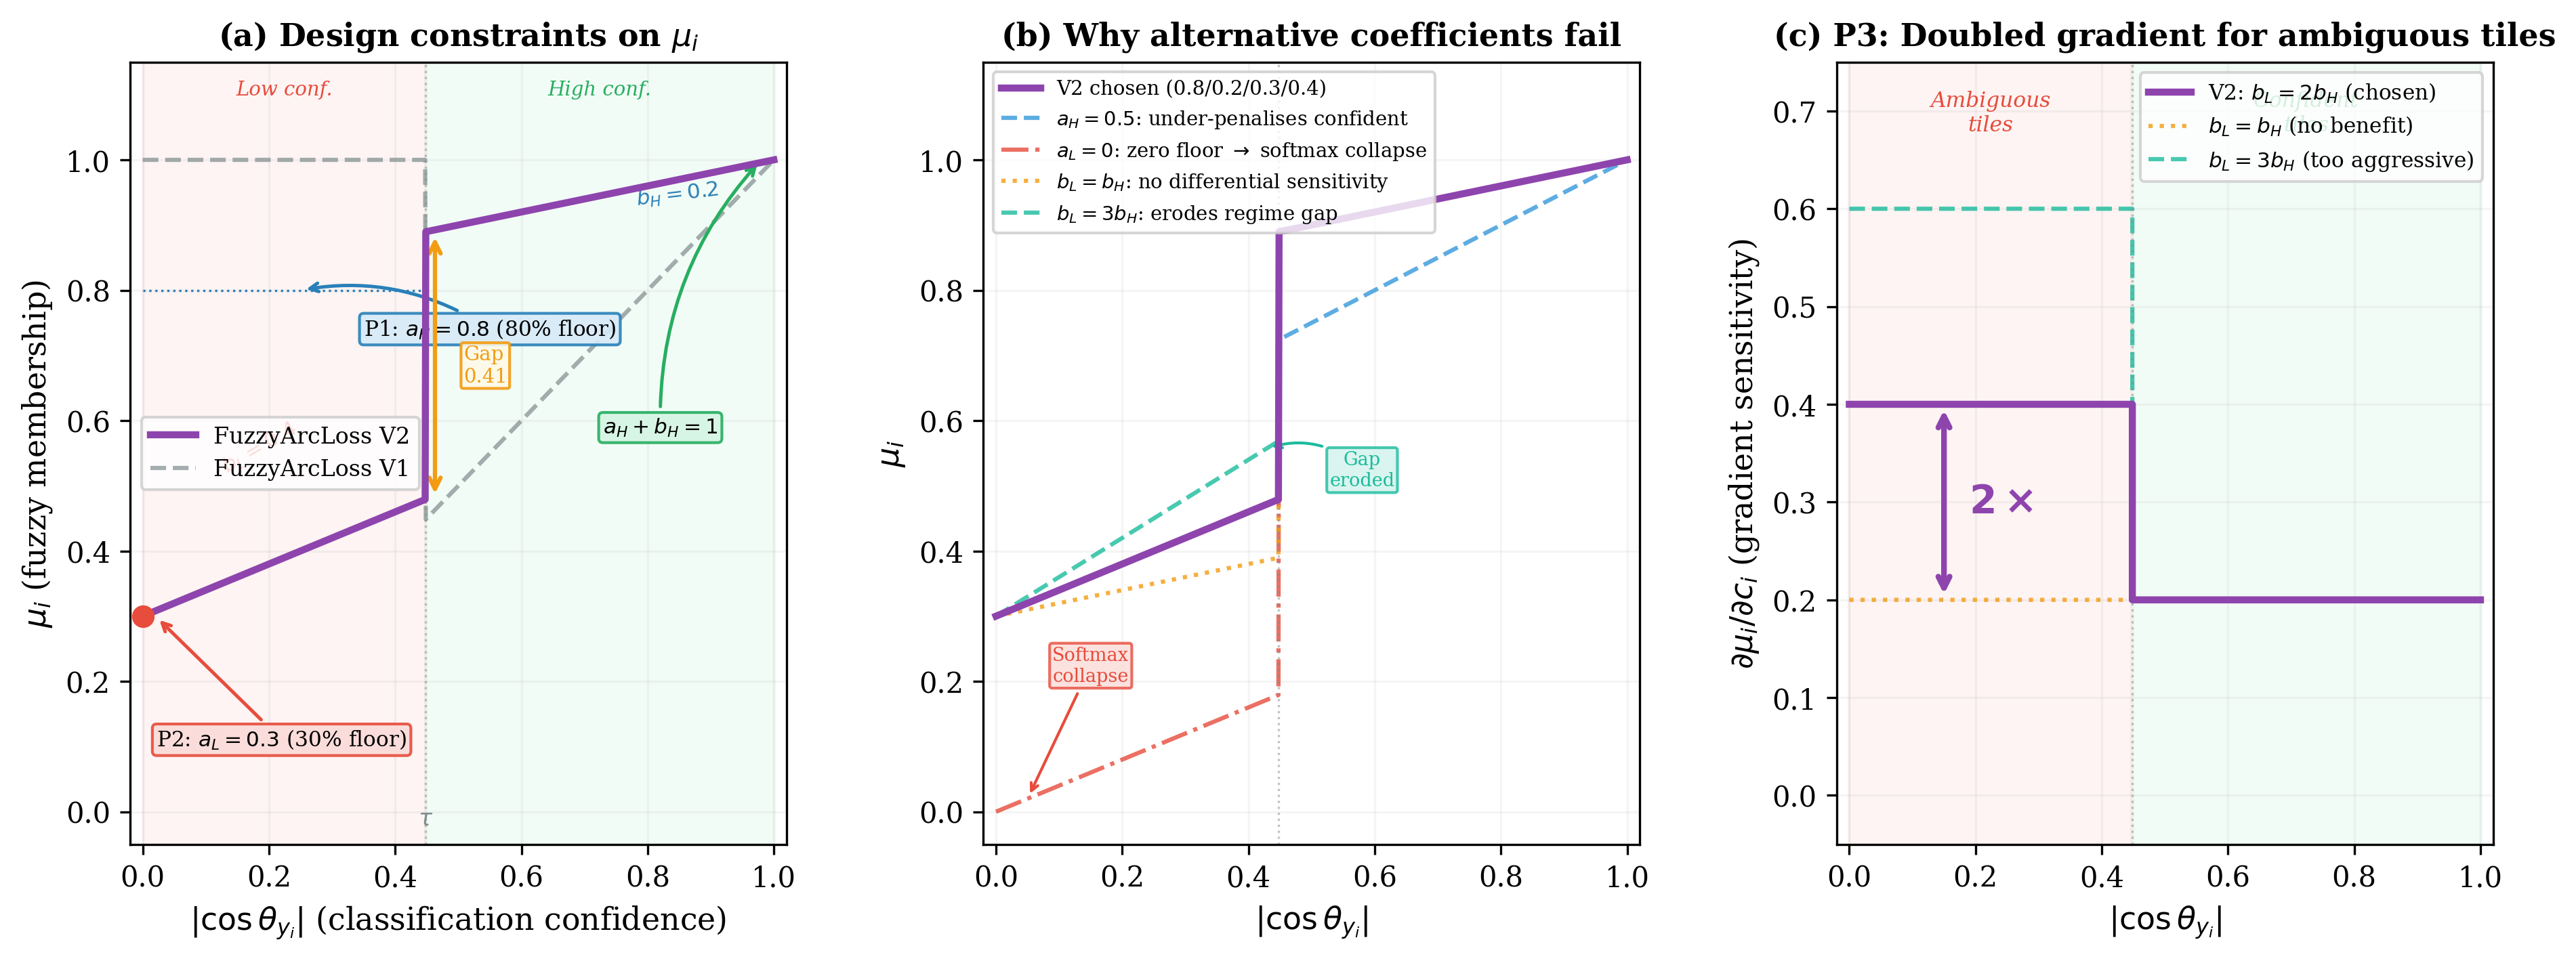
\includegraphics[width=\textwidth]{chapters/figures/fuzzyarcloss_v2_coefficient_rationale.png}
\caption[Design rationale for FuzzyArcLoss~V2 membership coefficients]{%
    Design rationale for the four membership function coefficients.
    \textbf{(a)}~The chosen V2 membership (purple) with annotated
    design constraints: the hard constraint $a_H + b_H = 1$ (green),
    the 80\% high-confidence floor $a_H = 0.8$ (Principle~1, blue),
    the 30\% global floor $a_L = 0.3$ (Principle~2, red), and the
    gap of 0.41 at $\tau$ between regimes.
    The V1 membership (grey dashed) is shown for comparison: V1
    assigns full margin ($\mu = 1$) to uncertain samples, while V2
    inverts this behaviour.
    \textbf{(b)}~Alternative coefficient choices and their failure
    modes: $a_H = 0.5$ under-penalises confident samples (blue
    dashed); $a_L = 0$ causes softmax collapse (red dash-dot);
    $b_L = b_H$ eliminates differential sensitivity (orange dotted);
    $b_L = 3 b_H$ erodes the gap between regimes (teal dashed).
    \textbf{(c)}~Gradient sensitivity
    $\partial \mu_i / \partial c_i$ showing Principle~3: the chosen
    design (purple) produces exactly $2\times$ the gradient correction
    for ambiguous tiles (red region) compared to confident ones (green
    region), creating a smoother optimisation landscape at
    morphological pattern boundaries.}
\label{fig:coeff_rationale}
\end{figure}

\textbf{Sensitivity and scope.}
These coefficients were fixed before the Optuna hyperparameter
search (Section~\ref{sec:meth:pattern:optuna}), which optimised
$s$, $m$, and $\tau$ conditioned on the fixed membership shape.
A sensitivity analysis varying $a_H \in \{0.7, 0.8, 0.9\}$ and
$b_L / b_H \in \{1, 2, 3\}$ is identified as short-term future
work (Section~\ref{sec:disc:future:short}).
The current configuration achieves 92.31\% macro-F1
($p = 0.001$ vs SphereFace, Cohen's $d = 1.00$), demonstrating
that the principled design is effective even without exhaustive
coefficient tuning.

\paragraph{Inversion relative to FuzzyArcLoss V1.}
A critical difference from V1~\cite{lima2025fuzzy} is that V2
\emph{inverts} the relationship between confidence and margin.
V1 assigns $\mu = 1$ (full margin) to uncertain samples and
$\mu = |\cos\theta|$ (reduced margin) to confident ones.
This design was appropriate for face recognition, where uncertain
samples are typically mislabelled or low-quality images that
benefit from aggressive angular separation.
In histopathology, however, uncertain samples are often tiles at
\emph{genuine morphological boundaries} (e.g., acinar--papillary
transitions) where the ground truth itself is ambiguous
($\kappa = 0.38$ inter-observer agreement~\cite{thunnissen2012reproducibility}).
Applying full margin to these tiles forces the model to memorise
the pathologist's arbitrary label rather than learning the
underlying continuous morphological spectrum.
V2's inversion---gentle margins for ambiguous tiles, strong
margins for confident ones---respects this biological gradience
and was empirically validated in the ablation study
(V2: 92.31\% vs V1: 90.47\% macro-F1).

\subsubsection{Modulated Target Logit}

In the implemented formulation, the fuzzy membership $\mu_i$ is
\emph{not} applied by replacing $m$ with $\mu_i m$ inside
$\cos(\theta + m)$.
Instead, $\mu_i$ is used to \emph{interpolate} between the
ArcFace-transformed target logit $\phi_i$ and the plain cosine target
logit $c_i$:
\begin{equation}
\label{eq:fuzzyarcloss_v2_method}
\tilde{z}_{y_i,i} = \mu_i \, \phi_i + (1 - \mu_i) \, c_i,
\end{equation}
where $\phi_i = \cos(\theta_{y_i} + m)$ is the standard ArcFace target
logit (with boundary correction) and $c_i = \cos\theta_{y_i}$ is the
margin-free cosine.
Non-target logits remain unchanged: $\tilde{z}_{k,i} = c_{k,i}$ for
$k \neq y_i$.

Figure~\ref{fig:fuzzyarcloss_v2_diagram} illustrates the complete mechanism.
This produces a clear interpretation:
\begin{itemize}
    \item If $\mu_i \approx 1$ (confident sample): $\tilde{z}_{y_i,i}
    \approx \phi_i$ --- standard ArcFace behaviour.
    \item If $\mu_i$ is small (ambiguous sample): $\tilde{z}_{y_i,i}$
    moves toward $c_i$ --- the angular margin is effectively reduced.
\end{itemize}

\begin{figure}[ht!]
\centering
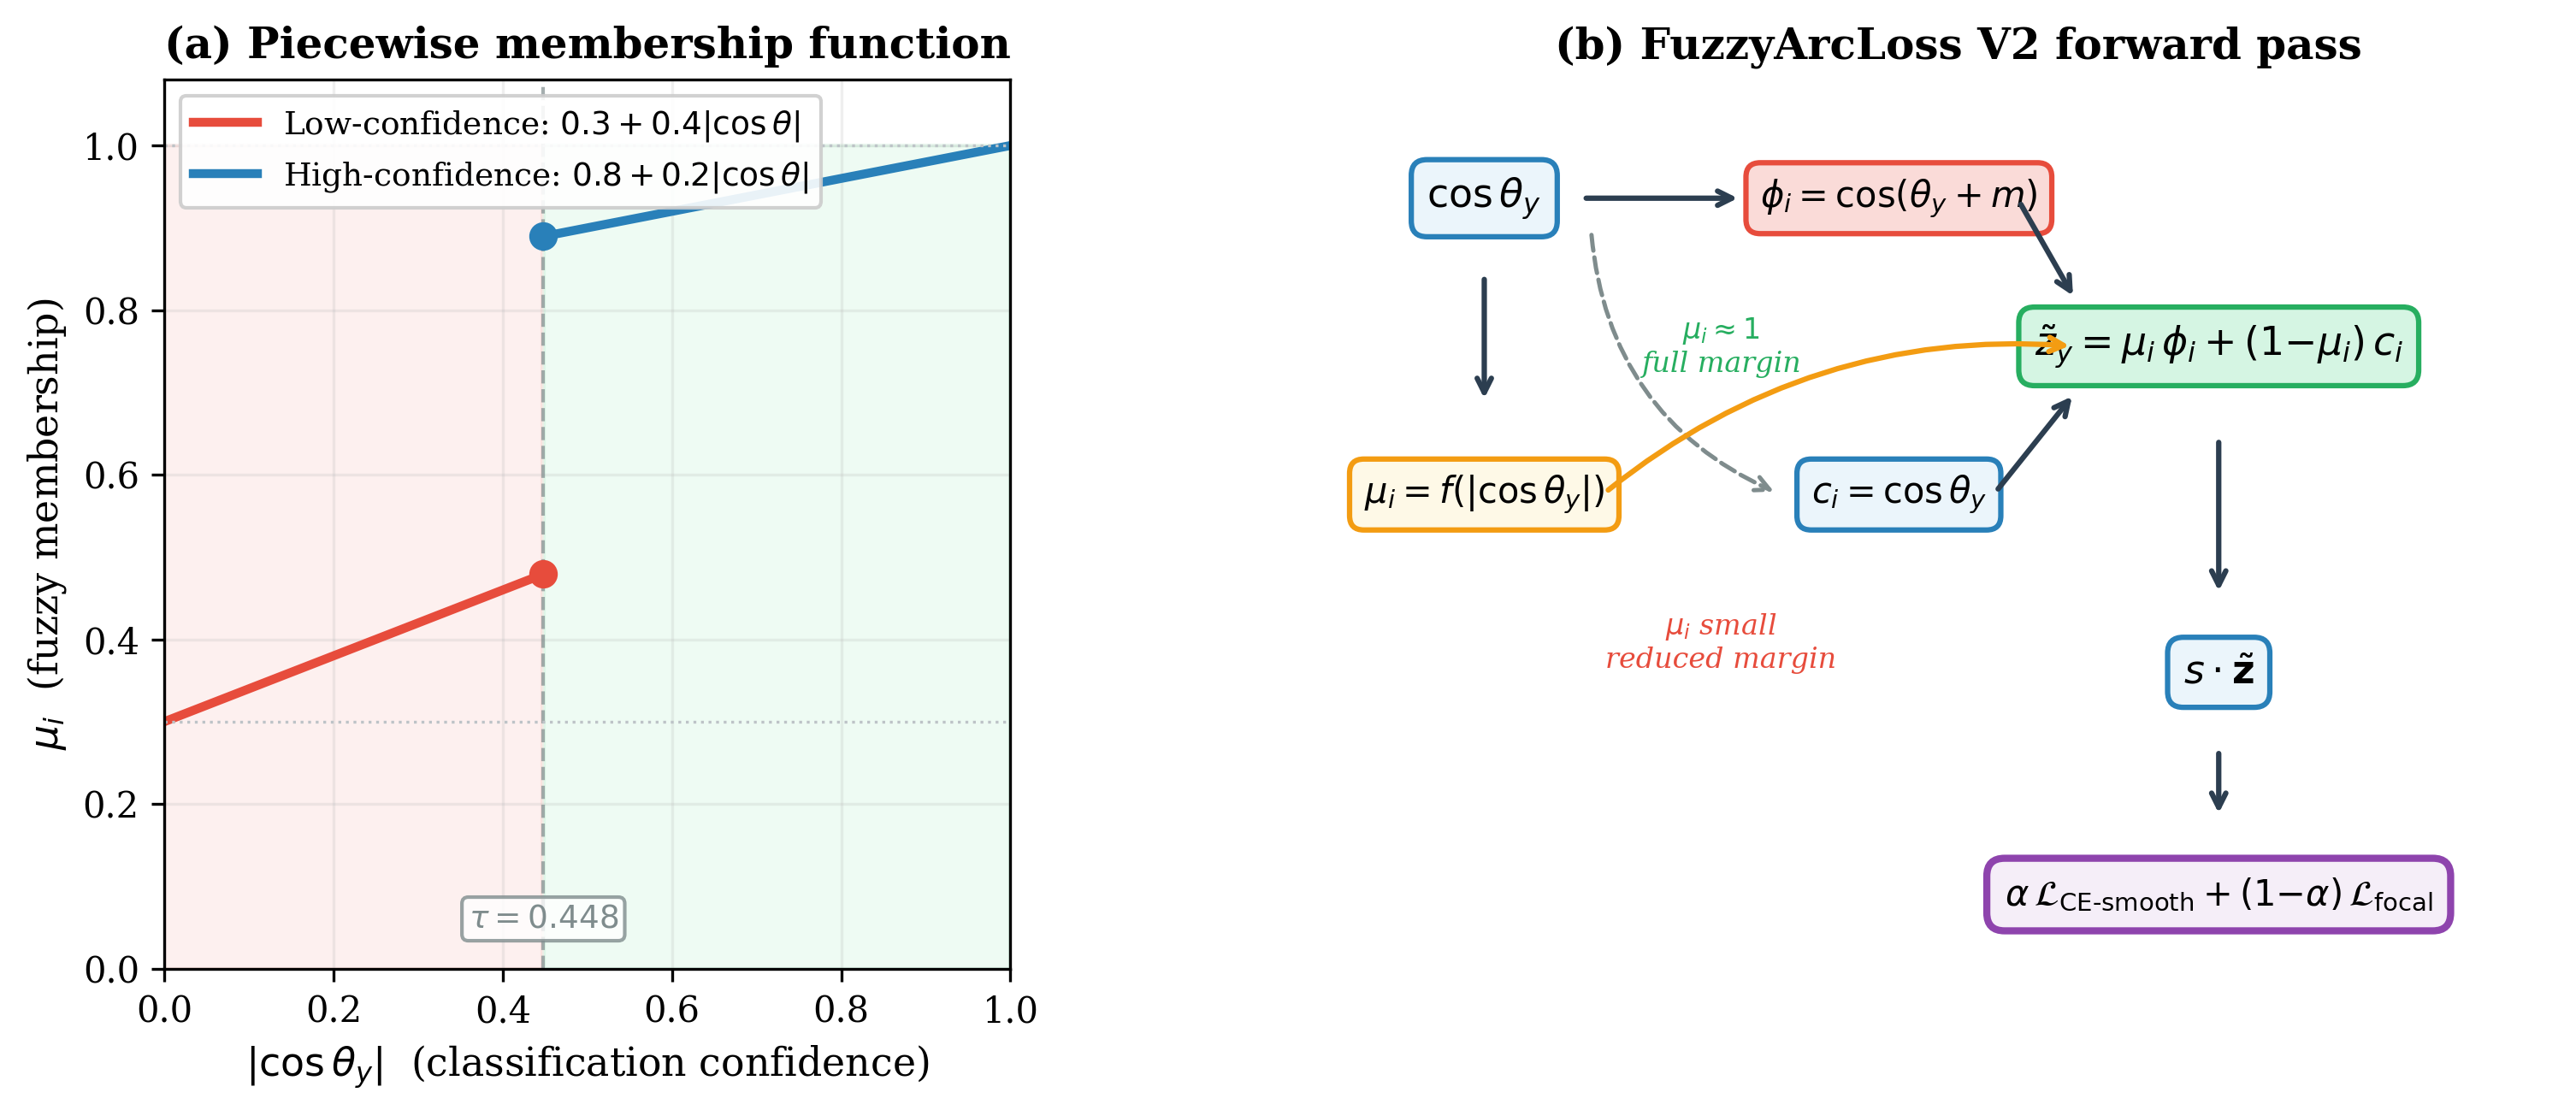
\includegraphics[width=\textwidth]{chapters/figures/fuzzyarcloss_v2_diagram.png}
\caption[FuzzyArcLoss~V2 mechanism: membership function and forward
pass.]{FuzzyArcLoss~V2 mechanism.
\textbf{(a)}~Piecewise linear membership function $\mu_i$ as a function of classification confidence $|\cos\theta_y|$.
The threshold $\tau = 0.448$ (Optuna-optimised) separates the high-confidence regime ($\mu \in [0.8, 1.0]$, blue) from the low-confidence regime ($\mu \in [0.3, 0.7]$, red).
\textbf{(b)}~Forward pass: the fuzzy membership $\mu_i$ interpolates between the ArcFace target logit $\phi_i = \cos(\theta_y + m)$ and the margin-free cosine $c_i$, producing the modulated logit $\tilde{z}_y$ which is then scaled and passed through the combined loss.}
\label{fig:fuzzyarcloss_v2_diagram}
\end{figure}

\subsubsection{Combined Loss Function}

The final logits are scaled by $s$ and passed through a combined loss
that includes label smoothing cross-entropy and focal
loss~\cite{lin2017focal}:
\begin{equation}
\label{eq:fuzzyarcloss_v2_loss}
\mathcal{L}_i = \alpha \, \mathcal{L}_{\text{CE-smooth}}(s \tilde{\mathbf{z}}_i, y_i)
\;+\; (1 - \alpha) \, \mathcal{L}_{\text{focal}}(s \tilde{\mathbf{z}}_i, y_i),
\end{equation}
where $\alpha \in [0,1]$ is a balance hyperparameter
(its concrete value, together with $\epsilon$ and $\gamma$, is
reported in Table~\ref{tab:hyper_pattern_classifier} in
Chapter~\ref{ch:implementation}).
The two loss terms address complementary failure modes that arise
when training angular margin classifiers on small, class-imbalanced
histopathological datasets:

\textbf{Label smoothing}~\cite{szegedy2016rethinking}
replaces the hard one-hot target
$\mathbf{y} = [0, 1, 0, 0, 0, 0]$ with a softened distribution
$\tilde{\mathbf{y}} = [\tfrac{\epsilon}{K},\;
1 - \epsilon + \tfrac{\epsilon}{K},\;
\tfrac{\epsilon}{K}, \ldots]$,
where $K = 6$ is the number of pattern classes and $\epsilon$ is
the smoothing strength.
This prevents the model from producing overconfident predictions
that would otherwise lead to poorly calibrated probability vectors
downstream---particularly important because these probabilities
serve as the fuzzy pattern membership features
$\mathbf{p}_i \in \Delta^5$ consumed by Artefacts~2 and~3.

\textbf{Focal loss}~\cite{lin2017focal}
(focusing parameter $\gamma$) modulates the
per-sample loss by the factor $(1 - p_y)^\gamma$, where $p_y$ is
the predicted probability for the correct class.
For well-classified samples ($p_y$ close to 1), the modulating factor
is small (close to 0) and the per-sample loss is heavily
down-weighted; for misclassified samples ($p_y$ close to 0) the
factor remains close to 1 and the loss is essentially unattenuated.
This asymmetry concentrates the learning signal on hard examples,
which in the Zenodo--ANORAK dataset~\cite{anorak2024}
disproportionately belong to the minority cribriform and
micropapillary classes (55 training tiles each, 10.8\%).

\textbf{Complementarity with FuzzyArcLoss~V2.}
The three mechanisms operate at different levels and are
non-redundant:
(i)~the fuzzy membership $\mu_i$ modulates the \emph{angular margin
geometry} in the logit space, reducing the penalty for tiles at
morphological boundaries regardless of their class;
(ii)~label smoothing modulates the \emph{target distribution},
preventing overconfident gradients for all classes;
(iii)~focal loss modulates the \emph{per-sample loss magnitude},
re-weighting the contribution of easy versus hard examples across
the entire training set.
Together, they create a training regime in which ambiguous tiles
at pattern boundaries receive gentle margins (fuzzy), well-classified
majority-class tiles contribute less to the gradient (focal), and
all predictions avoid pathological overconfidence (smoothing)---three
properties essential for learning well-separated embeddings from
only 637 annotated tiles.

Figure~\ref{fig:combined_loss_effect} illustrates the individual
and combined effects of the two loss components.

\begin{figure}[ht!]
\centering
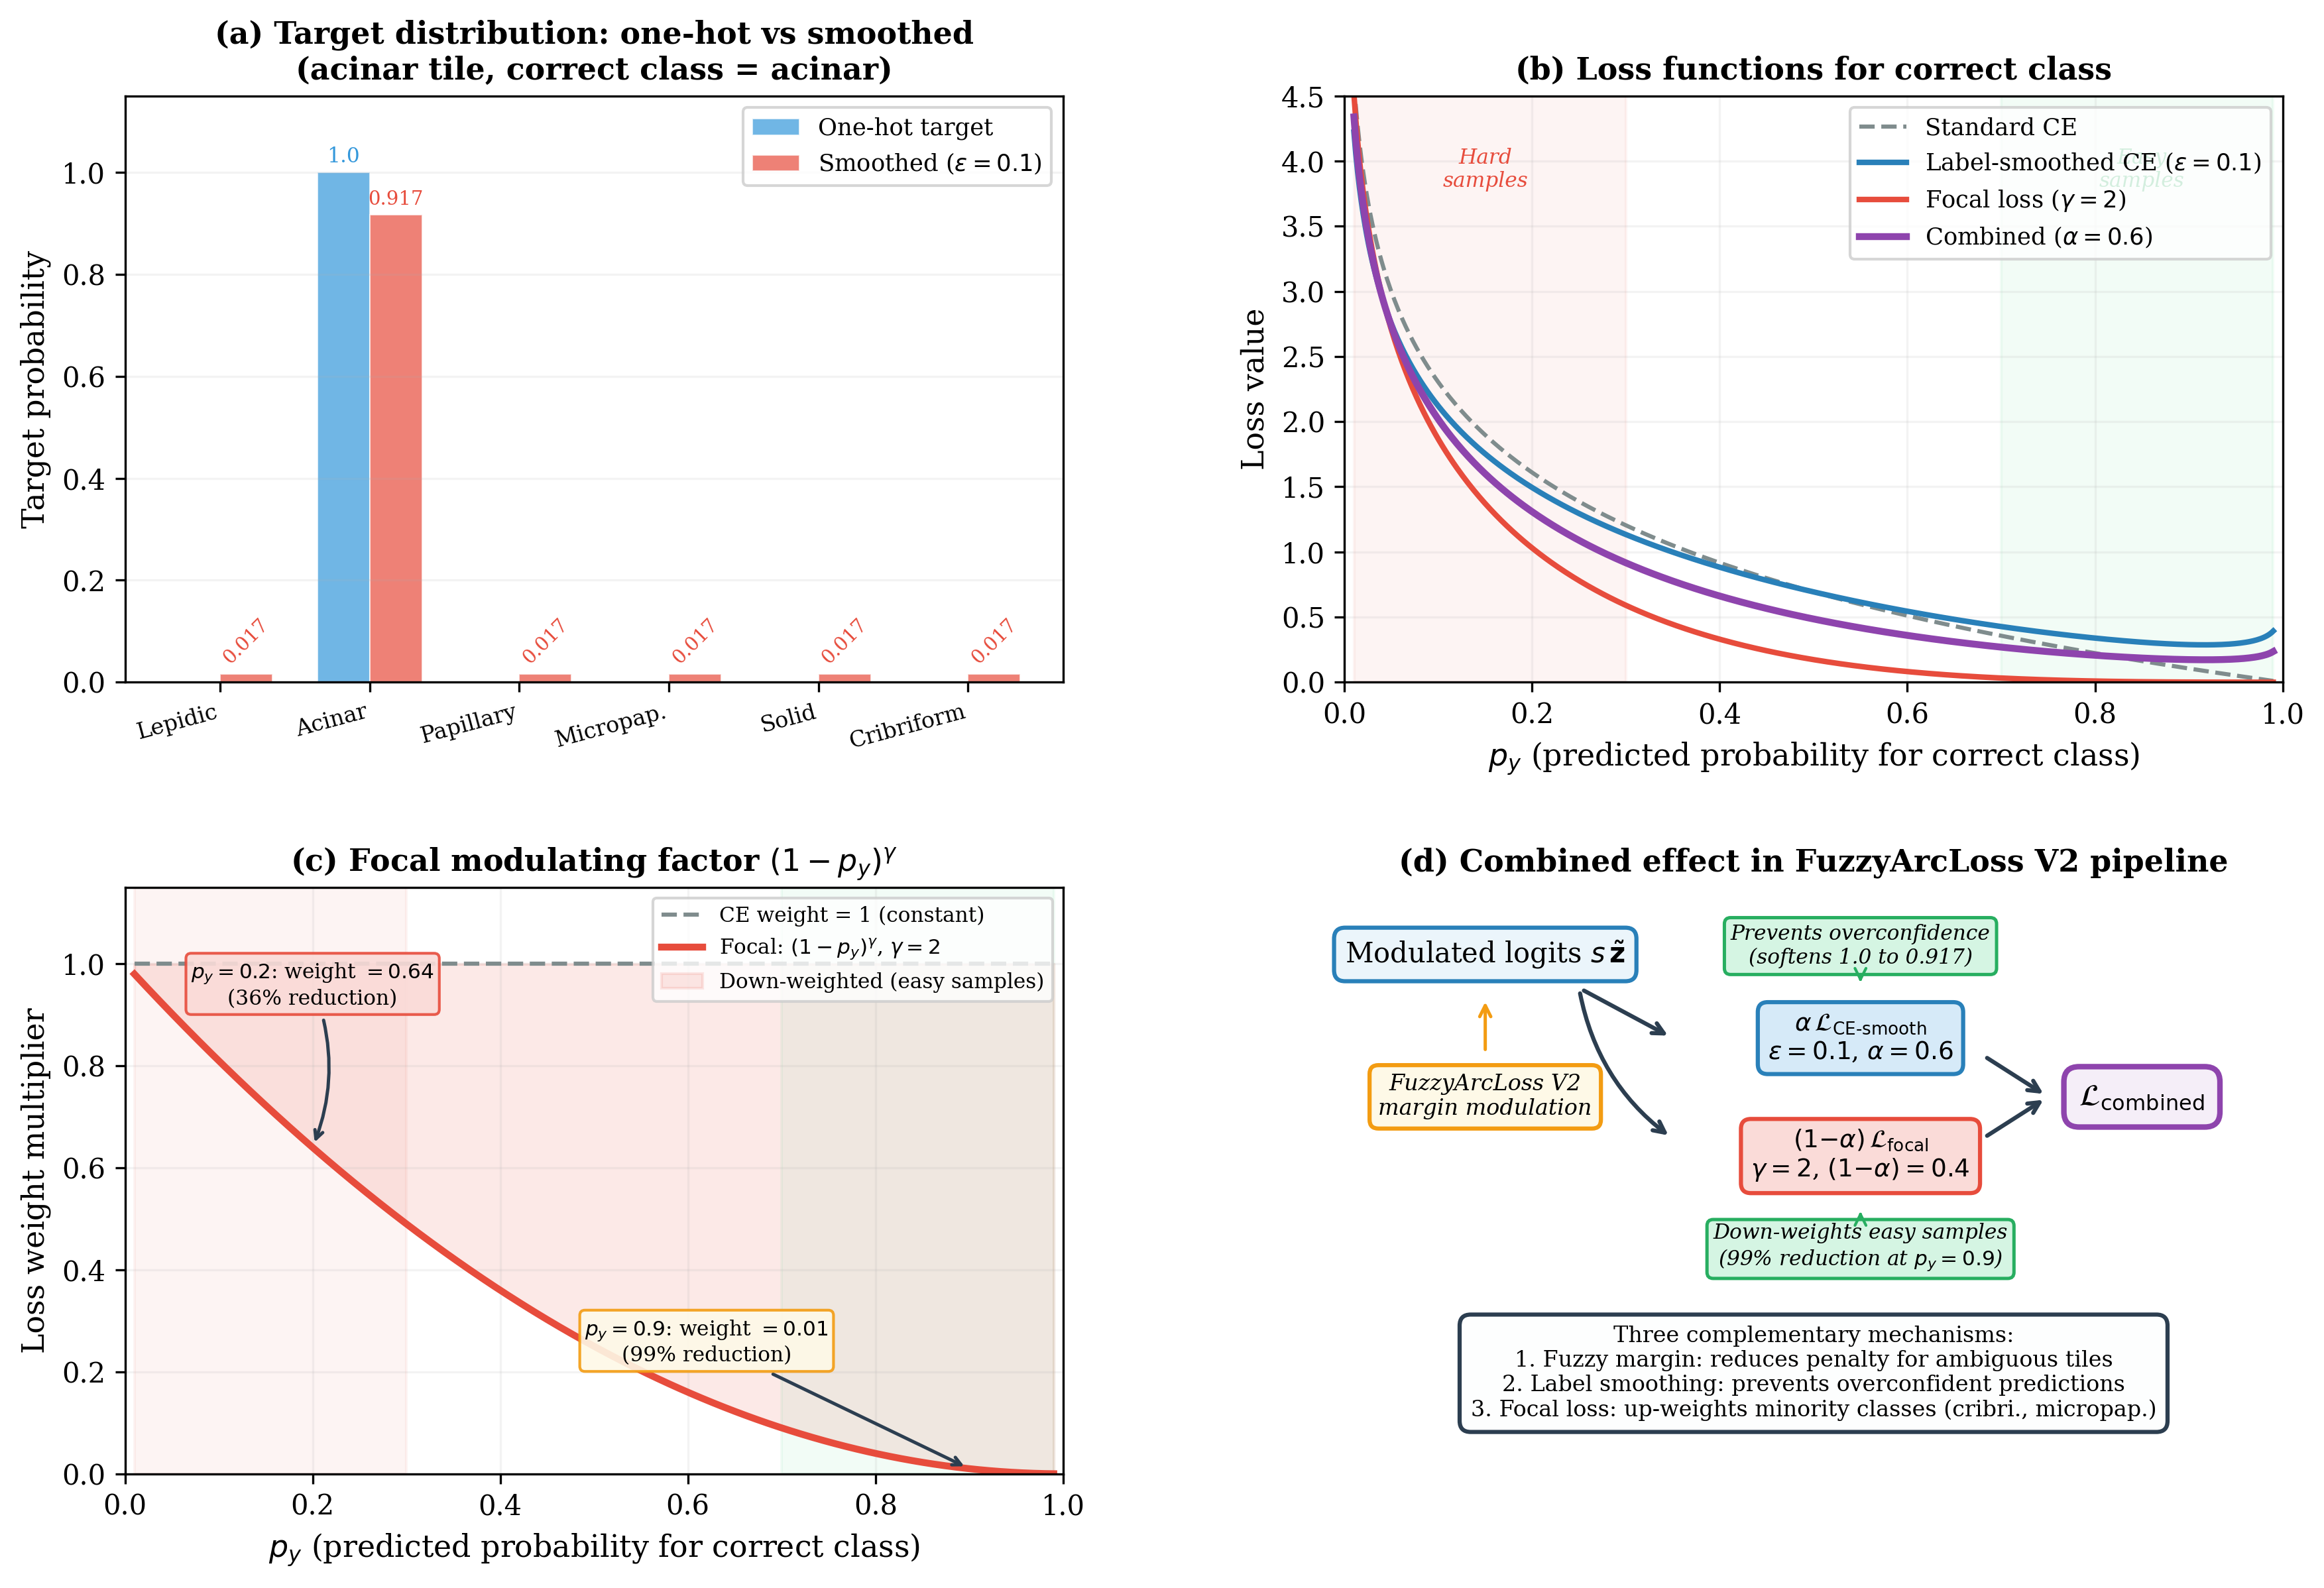
\includegraphics[width=\textwidth]{chapters/figures/fuzzyarcloss_v2_combined_loss.png}
\caption[Combined loss effect in FuzzyArcLoss~V2]{%
    Effect of the combined loss function
    (Equation~\ref{eq:fuzzyarcloss_v2_loss}).
    \textbf{(a)}~Target distribution for an acinar tile: the one-hot
    target (blue, correct class $= 1.0$) is softened by label smoothing
    ($\epsilon = 0.1$) to a distribution where the correct class
    receives $0.917$ and each incorrect class receives $0.017$ (red).
    \textbf{(b)}~Loss curves as a function of the predicted probability
    $p_y$ for the correct class: standard CE (grey dashed),
    label-smoothed CE (blue), focal loss (red), and the combined loss
    (purple, $\alpha = 0.6$).
    The combined loss inherits the focal term's aggressive
    down-weighting of easy samples (green region) while the
    label-smoothing component prevents overconfident predictions.
    \textbf{(c)}~Focal modulating factor $(1 - p_y)^\gamma$: at
    $p_y = 0.9$ the loss weight is reduced to 1\% of the CE baseline
    (99\% reduction), concentrating learning on hard examples from
    minority classes (cribriform, micropapillary).
    \textbf{(d)}~Block diagram showing how the three mechanisms
    (fuzzy margin, label smoothing, focal loss) are complementary
    and non-redundant in the FuzzyArcLoss~V2 pipeline.}
\label{fig:combined_loss_effect}
\end{figure}

\subsubsection{Gradient Analysis}
\label{sec:meth:pattern:fuzzyv2:gradient}

Differentiating the modulated target logit
(Equation~\ref{eq:fuzzyarcloss_v2_method}) with respect to the
target-class cosine $c_i$ yields
\begin{equation}
\label{eq:gradient}
\frac{\partial \tilde{z}_{y_i,i}}{\partial c_i}
= \mu_i \, \frac{\partial \phi_i}{\partial c_i}
+ (1 - \mu_i)
+ (\phi_i - c_i) \, \frac{\partial \mu_i}{\partial c_i},
\end{equation}
which separates three effects: (i)~the ArcFace contribution scaled by
$\mu_i$, (ii)~the direct cosine contribution scaled by $(1-\mu_i)$,
and (iii)~an adaptive term arising because $\mu_i$ itself depends on
$c_i$.
The derivative $\frac{\partial \mu_i}{\partial c_i}$ is $0.2$ in the
high-confidence regime ($|c_i| \ge \tau$) and $0.4$ in the
low-confidence regime ($|c_i| < \tau$), producing a \emph{larger
adaptive correction for ambiguous samples}.
This means the interpolation formulation not only reduces the effective
margin for uncertain tiles but also creates a smoother optimisation
landscape near decision boundaries---precisely the regions where
histological patterns overlap.

\paragraph{Derivation.}
The result in Equation~\ref{eq:gradient} follows from the product rule
applied to the interpolation formula
(Equation~\ref{eq:fuzzyarcloss_v2_method}).
Expanding $\tilde{z}_{y_i,i} = \mu_i \, \phi_i + c_i - \mu_i \, c_i$
and differentiating term by term with respect to $c_i$:
\begin{align}
\frac{\partial \tilde{z}_{y_i,i}}{\partial c_i}
&= \frac{\partial(\mu_i \, \phi_i)}{\partial c_i}
 + \frac{\partial(c_i)}{\partial c_i}
 - \frac{\partial(\mu_i \, c_i)}{\partial c_i} \notag \\[4pt]
&= \underbrace{\left(\frac{\partial \mu_i}{\partial c_i}\,\phi_i
   + \mu_i\,\frac{\partial \phi_i}{\partial c_i}\right)}_{\text{product rule on }\mu_i\phi_i}
 + \; 1
 - \underbrace{\left(\frac{\partial \mu_i}{\partial c_i}\,c_i
   + \mu_i\right)}_{\text{product rule on }\mu_i c_i} \notag \\[4pt]
&= \mu_i \, \frac{\partial \phi_i}{\partial c_i}
 + (1 - \mu_i)
 + \frac{\partial \mu_i}{\partial c_i}\,(\phi_i - c_i),
\label{eq:gradient_derived}
\end{align}
where the last line collects the $\frac{\partial \mu_i}{\partial c_i}$
terms.
The three resulting components have distinct roles:
\begin{itemize}
    \item \textbf{Term~(i)} $\mu_i \, \frac{\partial \phi_i}{\partial c_i}$:
    the standard ArcFace gradient, attenuated by the fuzzy membership.
    For confident samples ($\mu_i \approx 1$), this term dominates and
    the full angular margin is enforced.
    \item \textbf{Term~(ii)} $(1 - \mu_i)$:
    the direct cosine gradient, which increases for ambiguous samples
    (low $\mu_i$) and vanishes for confident ones.
    This term acts as a ``margin-free fallback'' that stabilises training
    near decision boundaries.
    \item \textbf{Term~(iii)} $(\phi_i - c_i)\,\frac{\partial \mu_i}{\partial c_i}$:
    the adaptive correction arising because $\mu_i$ itself is a function
    of $c_i$.
    Since $\phi_i < c_i$ (the ArcFace logit is always smaller than the
    margin-free cosine), $(\phi_i - c_i) < 0$, and this term is
    \emph{negative}---it further reduces the effective gradient for
    ambiguous samples.
    Crucially, $\frac{\partial \mu_i}{\partial c_i} = 0.4$ in the
    low-confidence regime versus $0.2$ in the high-confidence regime,
    so the adaptive correction is \emph{twice as large} for the samples
    that need it most.
\end{itemize}

Figure~\ref{fig:gradient_decomposition} visualises the three terms,
the total gradient comparison with standard ArcFace, and the effective
margin strength across the confidence spectrum.
The shaded area in panel~(b) quantifies the gradient reduction that
FuzzyArcLoss~V2 provides for low-confidence samples---the ``safety
valve'' that permits the aggressive Optuna-optimised scale
$s = 46.1$ without training instability.

\begin{figure}[ht!]
\centering
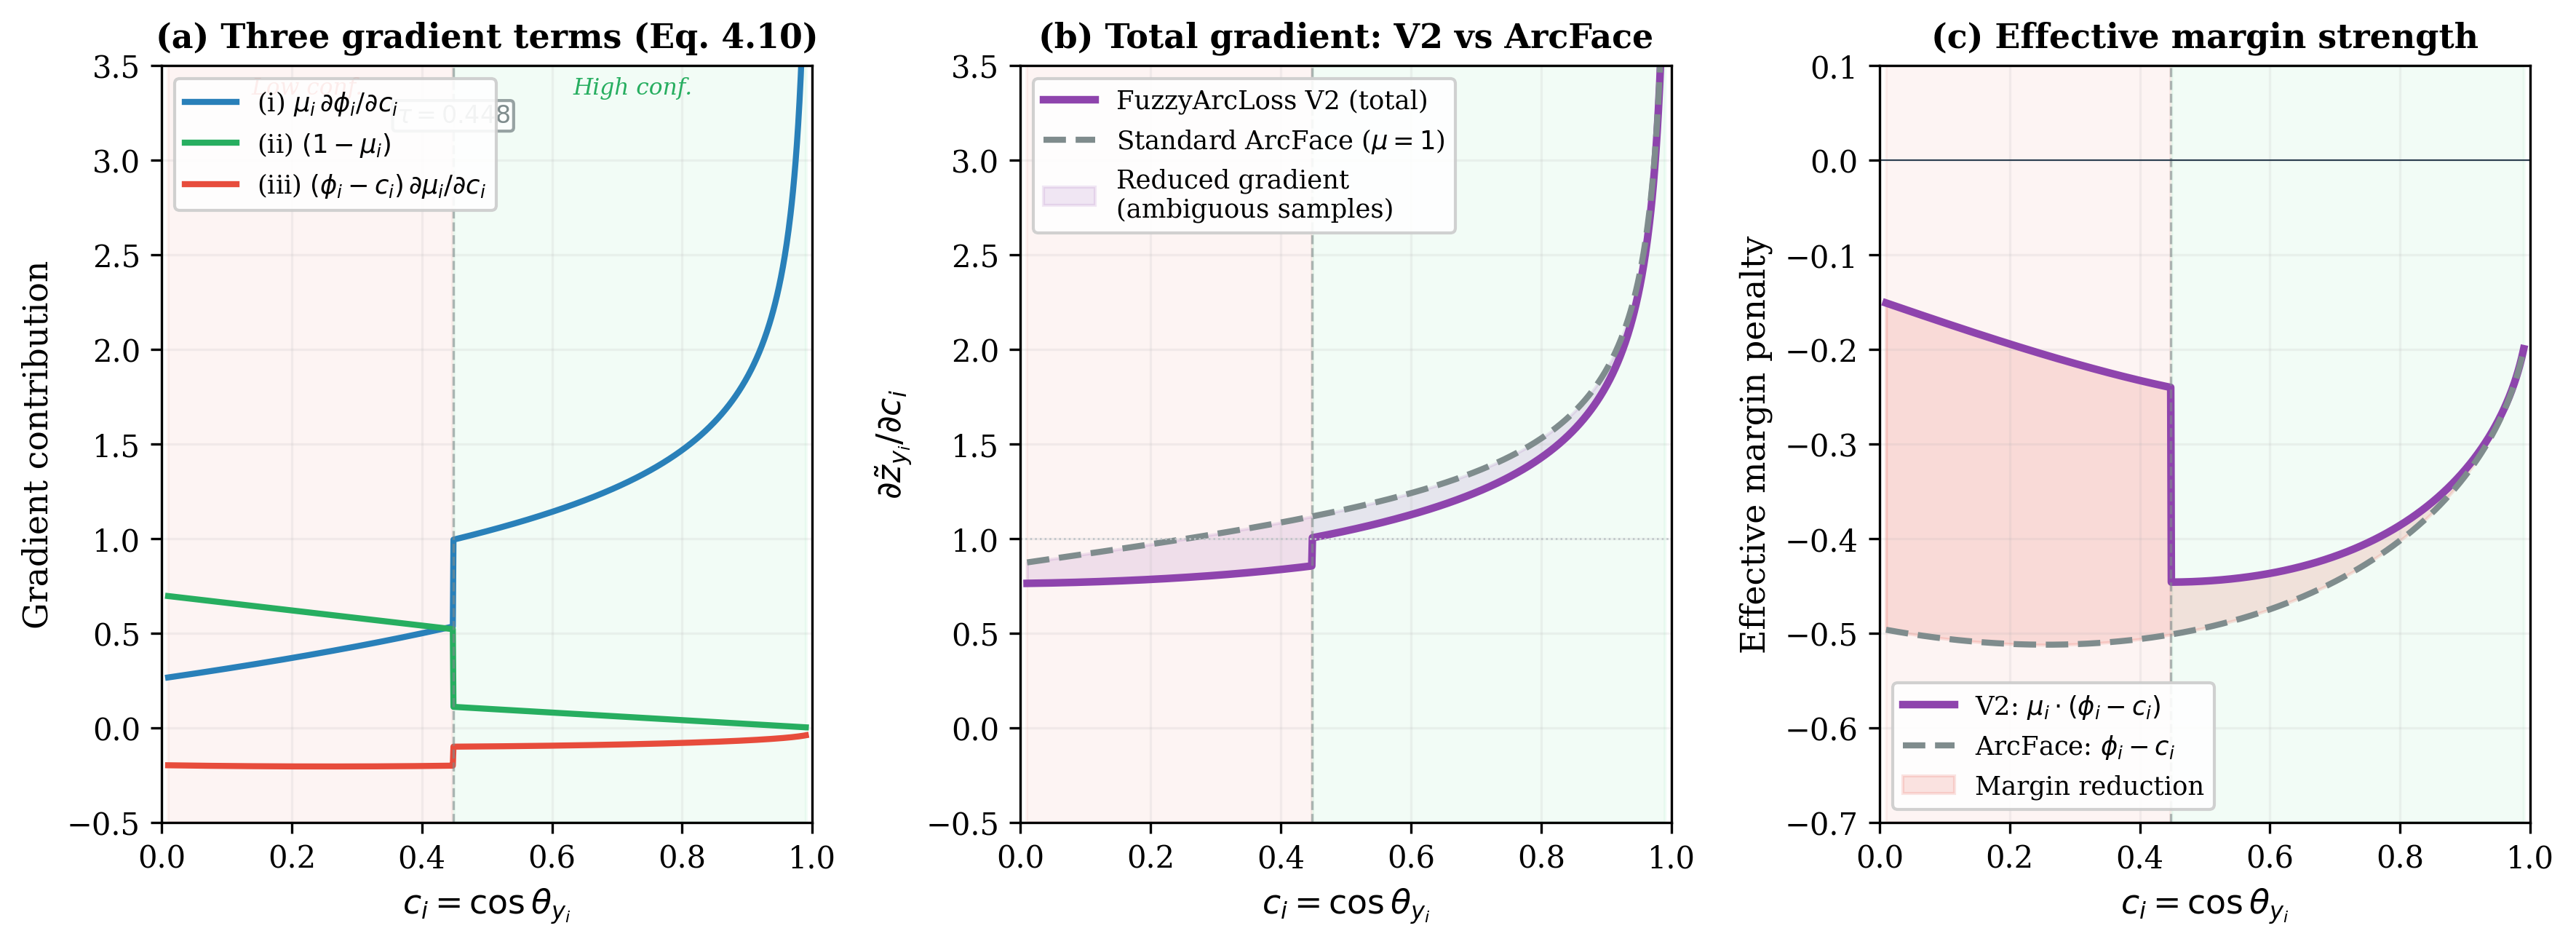
\includegraphics[width=\textwidth]{chapters/figures/fuzzyarcloss_v2_gradient_decomposition.png}
\caption[Gradient decomposition of FuzzyArcLoss~V2]{%
    Gradient decomposition of the modulated target logit
    (Equation~\ref{eq:gradient_derived}).
    \textbf{(a)}~The three terms as functions of
    $c_i = \cos\theta_{y_i}$:
    term~(i) is the ArcFace contribution scaled by $\mu_i$ (blue);
    term~(ii) is the direct cosine contribution (green);
    term~(iii) is the adaptive correction (red), which is twice as
    large in the low-confidence regime (red shading, $0.4$)
    as in the high-confidence regime (green shading, $0.2$).
    \textbf{(b)}~Total gradient: FuzzyArcLoss~V2 (purple) produces
    a consistently reduced gradient relative to standard ArcFace
    (grey dashed) for low-confidence samples, preventing gradient
    explosion at decision boundaries.
    The shaded area quantifies this reduction.
    \textbf{(c)}~Effective margin penalty: V2 applies a softer
    margin than ArcFace across the entire confidence spectrum,
    with the largest reduction for ambiguous samples near
    morphological pattern boundaries.
    Hyperparameters: $s = 46.1$, $m = 0.518$,
    $\tau = 0.448$ (Optuna-optimised).}
\label{fig:gradient_decomposition}
\end{figure}

\subsubsection{Relationship to Other Adaptive Margins}

Table~\ref{tab:margin_comparison} compares FuzzyArcLoss~V2 with related adaptive margin approaches.

\begin{table}[ht!]
\centering
\small
\caption{Comparison of margin modulation strategies. $\cos\theta_y$ denotes the cosine similarity to the correct class. $\bar{c}_k$ is the class-level average difficulty in AdaptiveFace.}
\label{tab:margin_comparison}
\resizebox{\textwidth}{!}{%
\begin{tabular}{@{}llll@{}}
\toprule
\textbf{Method} & \textbf{Margin type} & \textbf{Adaptation level} & \textbf{Modulation signal} \\
\midrule
ArcFace~\cite{deng2019arcface} & Fixed additive & None & --- \\
CosFace~\cite{wang2018cosface} & Fixed cosine & None & --- \\
SphereFace~\cite{liu2017sphereface} & Fixed multiplicative & None & --- \\
AdaptiveFace~\cite{liu2019adaptiveface} & Class-adaptive & Per class & $\bar{c}_k$ (class difficulty) \\
CurricularFace~\cite{huang2020curricularface} & Curriculum-adaptive & Per sample & $t$ (EMA of $\cos\theta_y$) + sample $\cos\theta_j$ \\
\textbf{FuzzyArcLoss V2} & \textbf{Fuzzy interpolation} & \textbf{Per sample} & $\mu(\cos\theta_y)$ (confidence) \\
\bottomrule
\end{tabular}}
\end{table}

FuzzyArcLoss~V2 is distinguished by its \emph{sample-level, confidence-based} modulation through an explicit fuzzy membership function that interpolates between the full ArcFace logit and the margin-free cosine (Equation~\ref{eq:fuzzyarcloss_v2_method}).
AdaptiveFace~\cite{liu2019adaptiveface} adjusts margins per class but treats all samples within a class uniformly.
CurricularFace~\cite{huang2020curricularface} is also per-sample, but it modulates \emph{negative-class} logits based on an adaptive threshold $t$ (an exponential moving average of target cosine) that evolves during training; the target-class margin itself remains fixed at $m$.
In contrast, FuzzyArcLoss~V2 modulates the \emph{target-class} logit directly via the fuzzy membership $\mu_i$, which is a deterministic function of instantaneous classification confidence and requires no running statistics.
This produces a margin that varies both across samples and across
training epochs as the model improves.

\paragraph{Excluded methods and scope justification.}
Three additional angular margin methods from the face recognition
literature---VPL~\cite{deng2021vpl} (virtual prototype learning,
per-class), SphereFace2~\cite{wen2022sphereface2} (improved
multiplicative margin, fixed), and
UniFace~\cite{zhou2023uniface} (unified normalisation,
per-class)---were evaluated in a preliminary screening using the
same CTransPath backbone, Zenodo--ANORAK dataset, and training
pipeline as the 18~losses in the final benchmark.
All three underperformed FuzzyArcLoss~V2 by substantial margins:
VPL ranked 13th (91.38\% F1), SphereFace2 ranked 15th (90.89\%),
and UniFace ranked last (89.08\%), compared to V2's 93.95\%
(differences of 2.6--4.9~pp, well beyond the $\pm 0.8$~pp
run-to-run variance).
Because these gaps exceeded the non-deterministic variation by a
factor of 3--6$\times$, these methods were excluded from the
computationally expensive 15-run K-fold evaluation
(Section~\ref{sec:meth:eval:cv}).

CurricularFace~\cite{huang2020curricularface} is the closest
literature comparator and was deliberately deferred rather than
included in this benchmark, on three grounds.
\emph{First}, the two losses solve categorically different
problems.
CurricularFace was designed for face recognition at the
million-image scale, where the optimisation pathology it targets
is the dominance of easy positives in early training; its
adaptive coefficient $t$ is therefore a \emph{single global}
exponential moving average of the target cosine that scales the
\emph{negative-class} logits over the course of training, leaving
the target-class margin fixed.
V2 was designed for the histopathology regime defined in
Section~\ref{sec:meth:pattern:fuzzyv2:membership}, where the
optimisation pathology is label noise from genuinely ambiguous
class boundaries (inter-observer
$\kappa = 0.38$~\cite{thunnissen2012reproducibility}); its
membership $\mu_i$ is a \emph{per-sample, instantaneous} function
of the sample's own cosine similarity that modulates the
\emph{target-class} logit and requires no running statistics.
The two methods therefore have opposite behaviour at the boundary:
CurricularFace progressively \emph{escalates} the angular pressure
on hard samples, whereas V2 progressively \emph{relaxes} it.
\emph{Second}, treating CurricularFace as ``the per-sample
adaptive baseline'' overstates the alignment.
The per-sample modulation in CurricularFace acts only through the
fixed EMA coefficient $t$ shared by all samples in a batch; this
is qualitatively different from V2's pathway, where each sample
sees a margin shaped by its own membership value (compare the
modulation-signal column of Table~\ref{tab:margin_comparison}).
\emph{Third}, including CurricularFace as a fair comparator would
require an additional hyperparameter sweep over its EMA momentum,
and that sweep would have to be run alongside the existing
$5 \times 3 = 15$-run protocol over the 18 losses already in
the benchmark---a compute budget that was not available within
this thesis but is straightforward at the scale of a follow-up
study.
The motivation to defer rather than discard is therefore not that
CurricularFace is uninformative, but that a like-for-like comparison
under matched hyperparameter budgets requires its own scoped
evaluation; this is documented explicitly as short-term future work
(Section~\ref{sec:disc:future:short}).


\subsection{FuzzyArcLoss V3: SubCenter Extension}
\label{sec:meth:pattern:fuzzyv3}

FuzzyArcLoss~V3 extends V2 by maintaining $C$ sub-center prototypes per class, each representing a morphological sub-cluster within the class.
The cosine similarity for class $k$ is computed against the nearest sub-center:
\begin{equation}
\label{eq:subcenter_method}
\cos\theta_k^{*} = \max_{c=1}^{C} \, \tilde{\mathbf{w}}_{k,c}^\top \tilde{\mathbf{x}},
\end{equation}
and the fuzzy membership modulation is applied to the resulting angle $\theta_k^{*}$.

With $C = 4$ sub-centers, V3 requires $K \times C \times d = 6 \times 4 \times 512 = 12{,}288$ prototype parameters, compared to $K \times d = 3{,}072$ for V2.
This four-fold increase in prototype parameters, combined with the limited training set (55--145 training tiles per class, mean $\sim$85; Table~\ref{tab:dataset_config_anorak}), leads to overfitting: V3 achieves 91.79\% macro-F1 versus V2's 92.31\% in 15-run evaluation (Section~\ref{ch:evaluation}).
V3 is therefore evaluated as an ablation condition rather than the primary proposed method.

Figure~\ref{fig:v3_subcenters} illustrates the geometric difference
between V2 and V3 on the angular embedding space, the parameter
count increase, and the resulting performance gap in the 15-run
K-fold evaluation.

\begin{figure}[ht!]
\centering
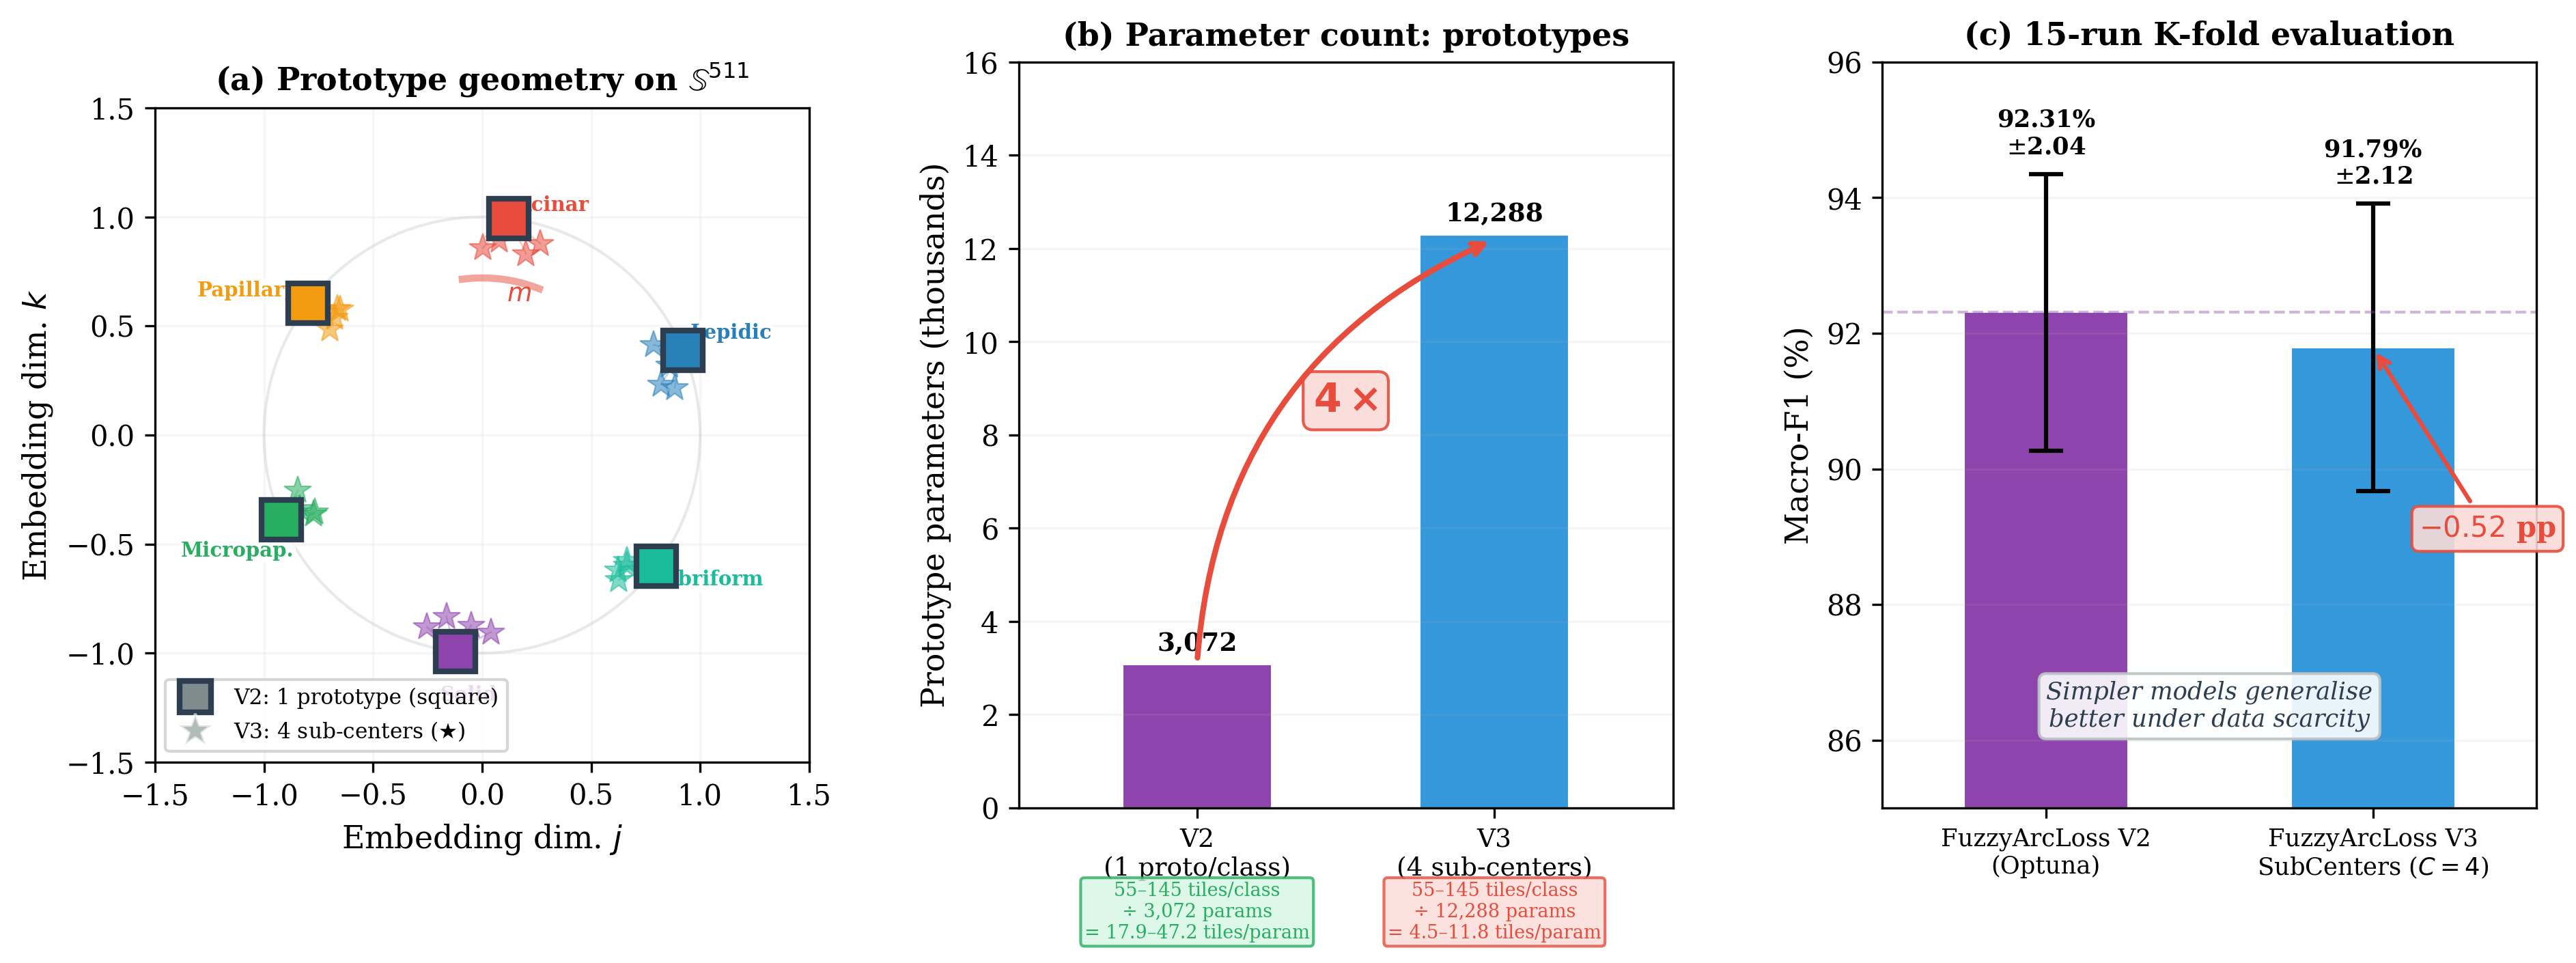
\includegraphics[width=\textwidth]{chapters/figures/fuzzyarcloss_v3_subcenters.png}
\caption[FuzzyArcLoss V3 SubCenter extension: geometry and overfitting]{%
    FuzzyArcLoss~V3 SubCenter extension compared to V2.
    \textbf{(a)}~Prototype geometry on a 2D slice of $\mathbb{S}^{511}$:
    V2 maintains one prototype per class (squares), while V3 adds $C = 4$
    sub-center prototypes (translucent circles) to capture intra-class
    morphological sub-clusters.
    The angular margin $m$ is applied relative to the nearest
    sub-center.
    \textbf{(b)}~Prototype parameter count: V3 requires $12{,}288$
    parameters ($4\times$ V2's $3{,}072$), reducing the effective
    samples-per-parameter ratio from $17.7$ to $4.4$---well below
    the threshold where overfitting becomes likely on 55--145 training
    tiles per class (mean $\sim$85).
    \textbf{(c)}~15-run K-fold evaluation: V3 achieves $91.79\%$
    macro-F1 versus V2's $92.31\%$ ($-0.52$\,pp), confirming that
    simpler models generalise better under data scarcity.}
\label{fig:v3_subcenters}
\end{figure}


\subsection{FuzzyArcLoss V2 ClassParams: Per-Class Margin Geometry}
\label{sec:meth:pattern:classparams}

A second variant, \textbf{FuzzyArcLoss~V2~ClassParams}, extends V2 by
replacing the global hyperparameters $m$ and $\tau$ with per-class
parameters $m_k$ and $\tau_k$ ($k = 1, \ldots, K$).
Each histological class can therefore define its own angular margin and
confidence threshold; for instance, a large margin may benefit the
well-separated \emph{solid} class while a smaller margin better suits
the morphologically ambiguous \emph{acinar--papillary} boundary.

With six LUAD classes, this adds $2 \times 6 = 12$ scalar
hyperparameters compared to V2's two.
In the single-run screening (Section~\ref{ch:evaluation}),
V2~ClassParams achieves 93.92\% macro-F1 (rank~4 of~18), but it was
excluded from the K-fold benchmark because the expanded Optuna search
space (12~class-specific values instead of~2 global ones) would require
disproportionate compute for limited expected gain.
V2~ClassParams is retained as a design reference for future work with
larger datasets.

Figure~\ref{fig:v2_classparams} illustrates the per-class membership
concept, the search space expansion, and the single-run screening
result that motivated the exclusion from the K-fold benchmark.

\begin{figure}[ht!]
\centering
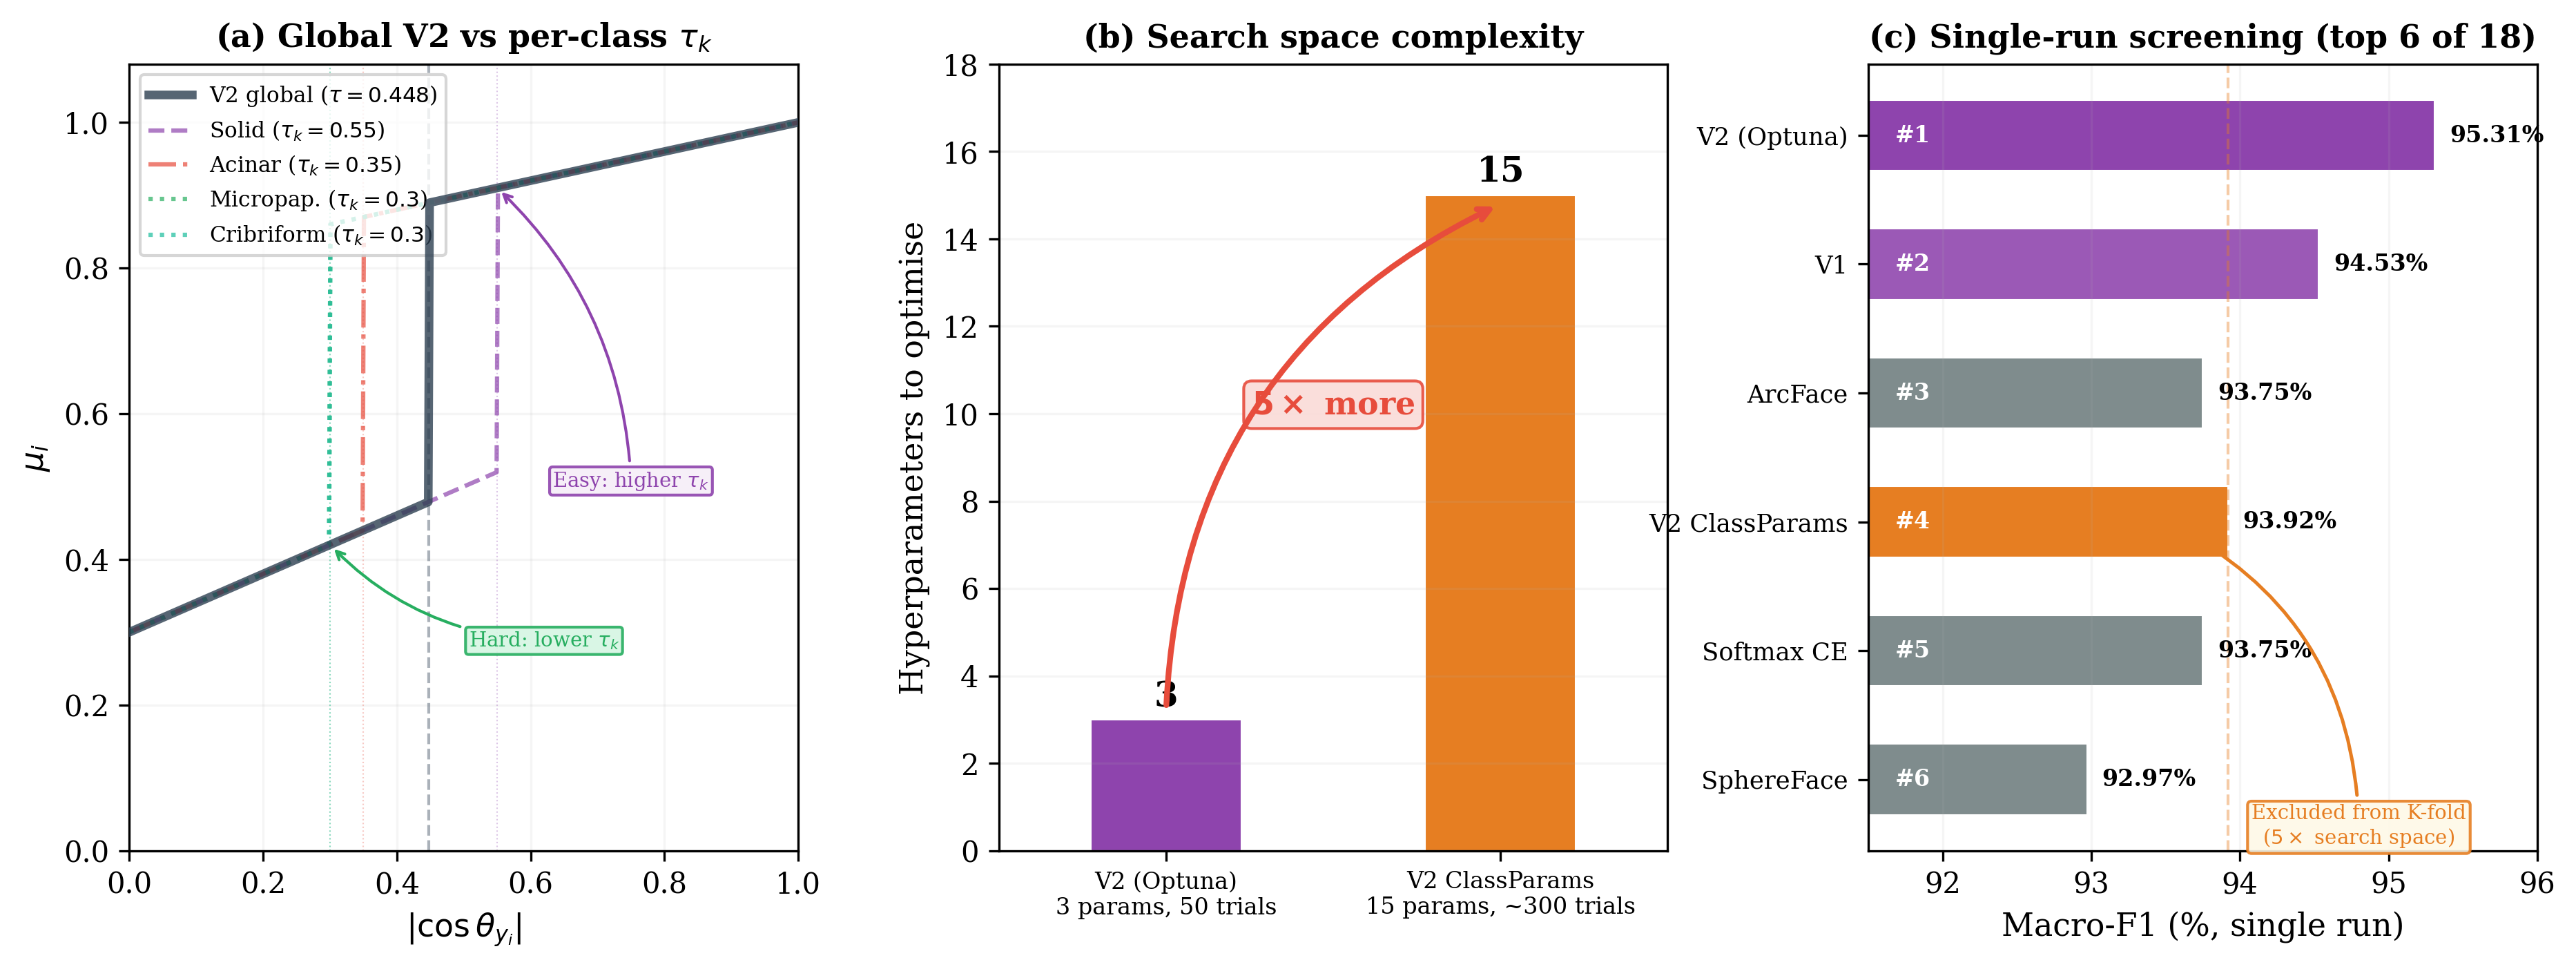
\includegraphics[width=\textwidth]{chapters/figures/fuzzyarcloss_v2_classparams.png}
\caption[FuzzyArcLoss V2 ClassParams: per-class margin geometry]{%
    FuzzyArcLoss~V2 ClassParams variant.
    \textbf{(a)}~Per-class membership functions: the global V2
    threshold $\tau = 0.448$ (black) is replaced by class-specific
    thresholds $\tau_k$.
    Easy classes (e.g., solid, $\tau_k = 0.55$) receive a stricter
    threshold---only highly confident samples get full margin---while
    hard classes (e.g., micropapillary, cribriform, $\tau_k = 0.30$)
    receive gentler thresholds that expand the high-confidence regime.
    \textbf{(b)}~Search space complexity: ClassParams introduces 15
    hyperparameters ($5\times$ more than V2's 3 global parameters),
    requiring $\sim$300+ Optuna trials for adequate coverage versus
    50 for V2.
    \textbf{(c)}~Single-run screening (top 6 of 18 loss functions):
    ClassParams ranks 4th with 93.92\% macro-F1, demonstrating
    competitive performance but excluded from the rigorous 15-run
    K-fold evaluation due to the disproportionate search space cost.}
\label{fig:v2_classparams}
\end{figure}


\subsection{Hyperparameter Optimisation with Optuna}
\label{sec:meth:pattern:optuna}

The three key hyperparameters of FuzzyArcLoss~V2---scale $s$, margin
$m$, and threshold $\tau$---are treated as a continuous joint design
choice and selected by Bayesian hyperparameter optimisation
(Optuna~\cite{akiba2019optuna} with the Tree-structured Parzen
Estimator~\cite{bergstra2011tpe}).
The methodological decisions captured at this layer are
(i)~\emph{which} parameters belong to the search space and
(ii)~\emph{what} validation objective the search optimises.
Concrete search ranges, number of trials, and pruning rule are
implementation details and are reported in
Section~\ref{sec:impl:pattern:optuna_config}.

\paragraph{Optimisation objective.}
Because the dataset is multi-class and imbalanced, the Optuna search
optimised a validation metric that directly captures the
precision--recall balance:
\begin{equation}
\label{eq:avgpr_optuna}
\mathrm{avgPR} = \frac{\mathrm{MacroPrecision} + \mathrm{MacroRecall}}{2}.
\end{equation}
Macro-averaging ensures that minority patterns (particularly cribriform
and micropapillary with $\sim$55 training tiles each out of 69 total;
Table~\ref{tab:dataset_config_anorak}) contribute equally to
the objective.
The search itself uses a deliberately truncated training protocol to
explore the $(s, m, \tau)$ space efficiently; once the optimum is
identified, the configuration is re-trained under the full protocol.
Concrete search-loop parameters (number of trials, per-trial epoch
budget, pruning rule, sampler) are reported in
Section~\ref{sec:impl:pattern:optuna_config}.
 
The Optuna-tuned values of $(s, m, \tau)$, together with the small set
of \emph{methodological} architectural decisions (4-channel input,
fp32 numerics, mixed-objective loss), are summarised in
Table~\ref{tab:hyper_fuzzyarc2}.
The remaining engineering hyperparameters of the training run
(learning rate, batch size, optimiser, scheduler, warmup, augmentation
flags, gradient clipping) are deferred to
Table~\ref{tab:hyper_pattern_classifier} in
Chapter~\ref{ch:implementation}, where they are reported as
implementation choices rather than design decisions.
 
\begin{table}[ht!]
\centering
\small
\caption{Methodological hyperparameters of the FuzzyArcLoss~V2
pattern classifier.
The three Optuna-optimised parameters $(s, m, \tau)$ are reported
alongside their ArcFace defaults; the remaining rows record
architectural decisions whose rationale is methodological.
Engineering-level training hyperparameters (LR, optimiser, scheduler,
batch size, augmentation) are listed in
Table~\ref{tab:hyper_pattern_classifier}.}
\label{tab:hyper_fuzzyarc2}
\begin{tabular}{l l c c}
\hline
\textbf{Parameter} & \textbf{Description} &
\textbf{ArcFace default} & \textbf{This work} \\
\hline
Scale $s$               & Logit scaling factor~\cite{deng2019arcface}                       & 30.0 & \textbf{46.1} \\
Margin $m$              & Angular margin (radians)~\cite{deng2019arcface}                   & 0.50 & \textbf{0.518} \\
Threshold $\tau$        & Confidence threshold for $\mu$~\cite{lima2025fuzzy}               & 0.50 & \textbf{0.448} \\
Input channels          & RGB + tissue mask (Sec.~\ref{sec:meth:mask_channel})              & 3    & 4 \\
Precision               & fp32 to preserve angular gradients (Sec.~\ref{sec:uc:pipeline_fixes}) & --- & fp32 \\
Combined loss           & $\alpha\,\mathcal{L}_{\text{CE-smooth}}$~\cite{szegedy2016rethinking} $+ (1-\alpha)\,\mathcal{L}_{\text{focal}}$~\cite{lin2017focal} & --- & yes \\
\hline
\end{tabular}
\end{table}


The optimal configuration identified was:
\begin{equation}
\label{eq:optuna_result}
s^* = 46.1, \quad m^* = 0.518, \quad \tau^* = 0.448.
\end{equation}

\textbf{Interpretation.}
The notably high scale ($s^* = 46.1$ versus the default $s = 30$ in standard ArcFace) is interpretable through the fuzzy membership mechanism.
A higher scale sharpens the softmax distribution, making the model more decisive.
In standard ArcFace, this would risk training instability for ambiguous samples.
In FuzzyArcLoss~V2, the fuzzy membership acts as a ``safety valve'': the reduced margin for uncertain samples ($\mu_i \approx 0.3$--$0.5$) compensates for the aggressive scale, preventing gradient explosion at decision boundaries.
The margin $m^* = 0.518$ is close to the ArcFace default ($m = 0.5$), confirming that the modulation mechanism---not the raw margin magnitude---is the source of V2's advantage.

Figure~\ref{fig:optuna_search} visualises the 50-trial search
process, showing the convergence behaviour and the relationship
between each hyperparameter and validation performance.

\begin{figure}[ht!]
\centering
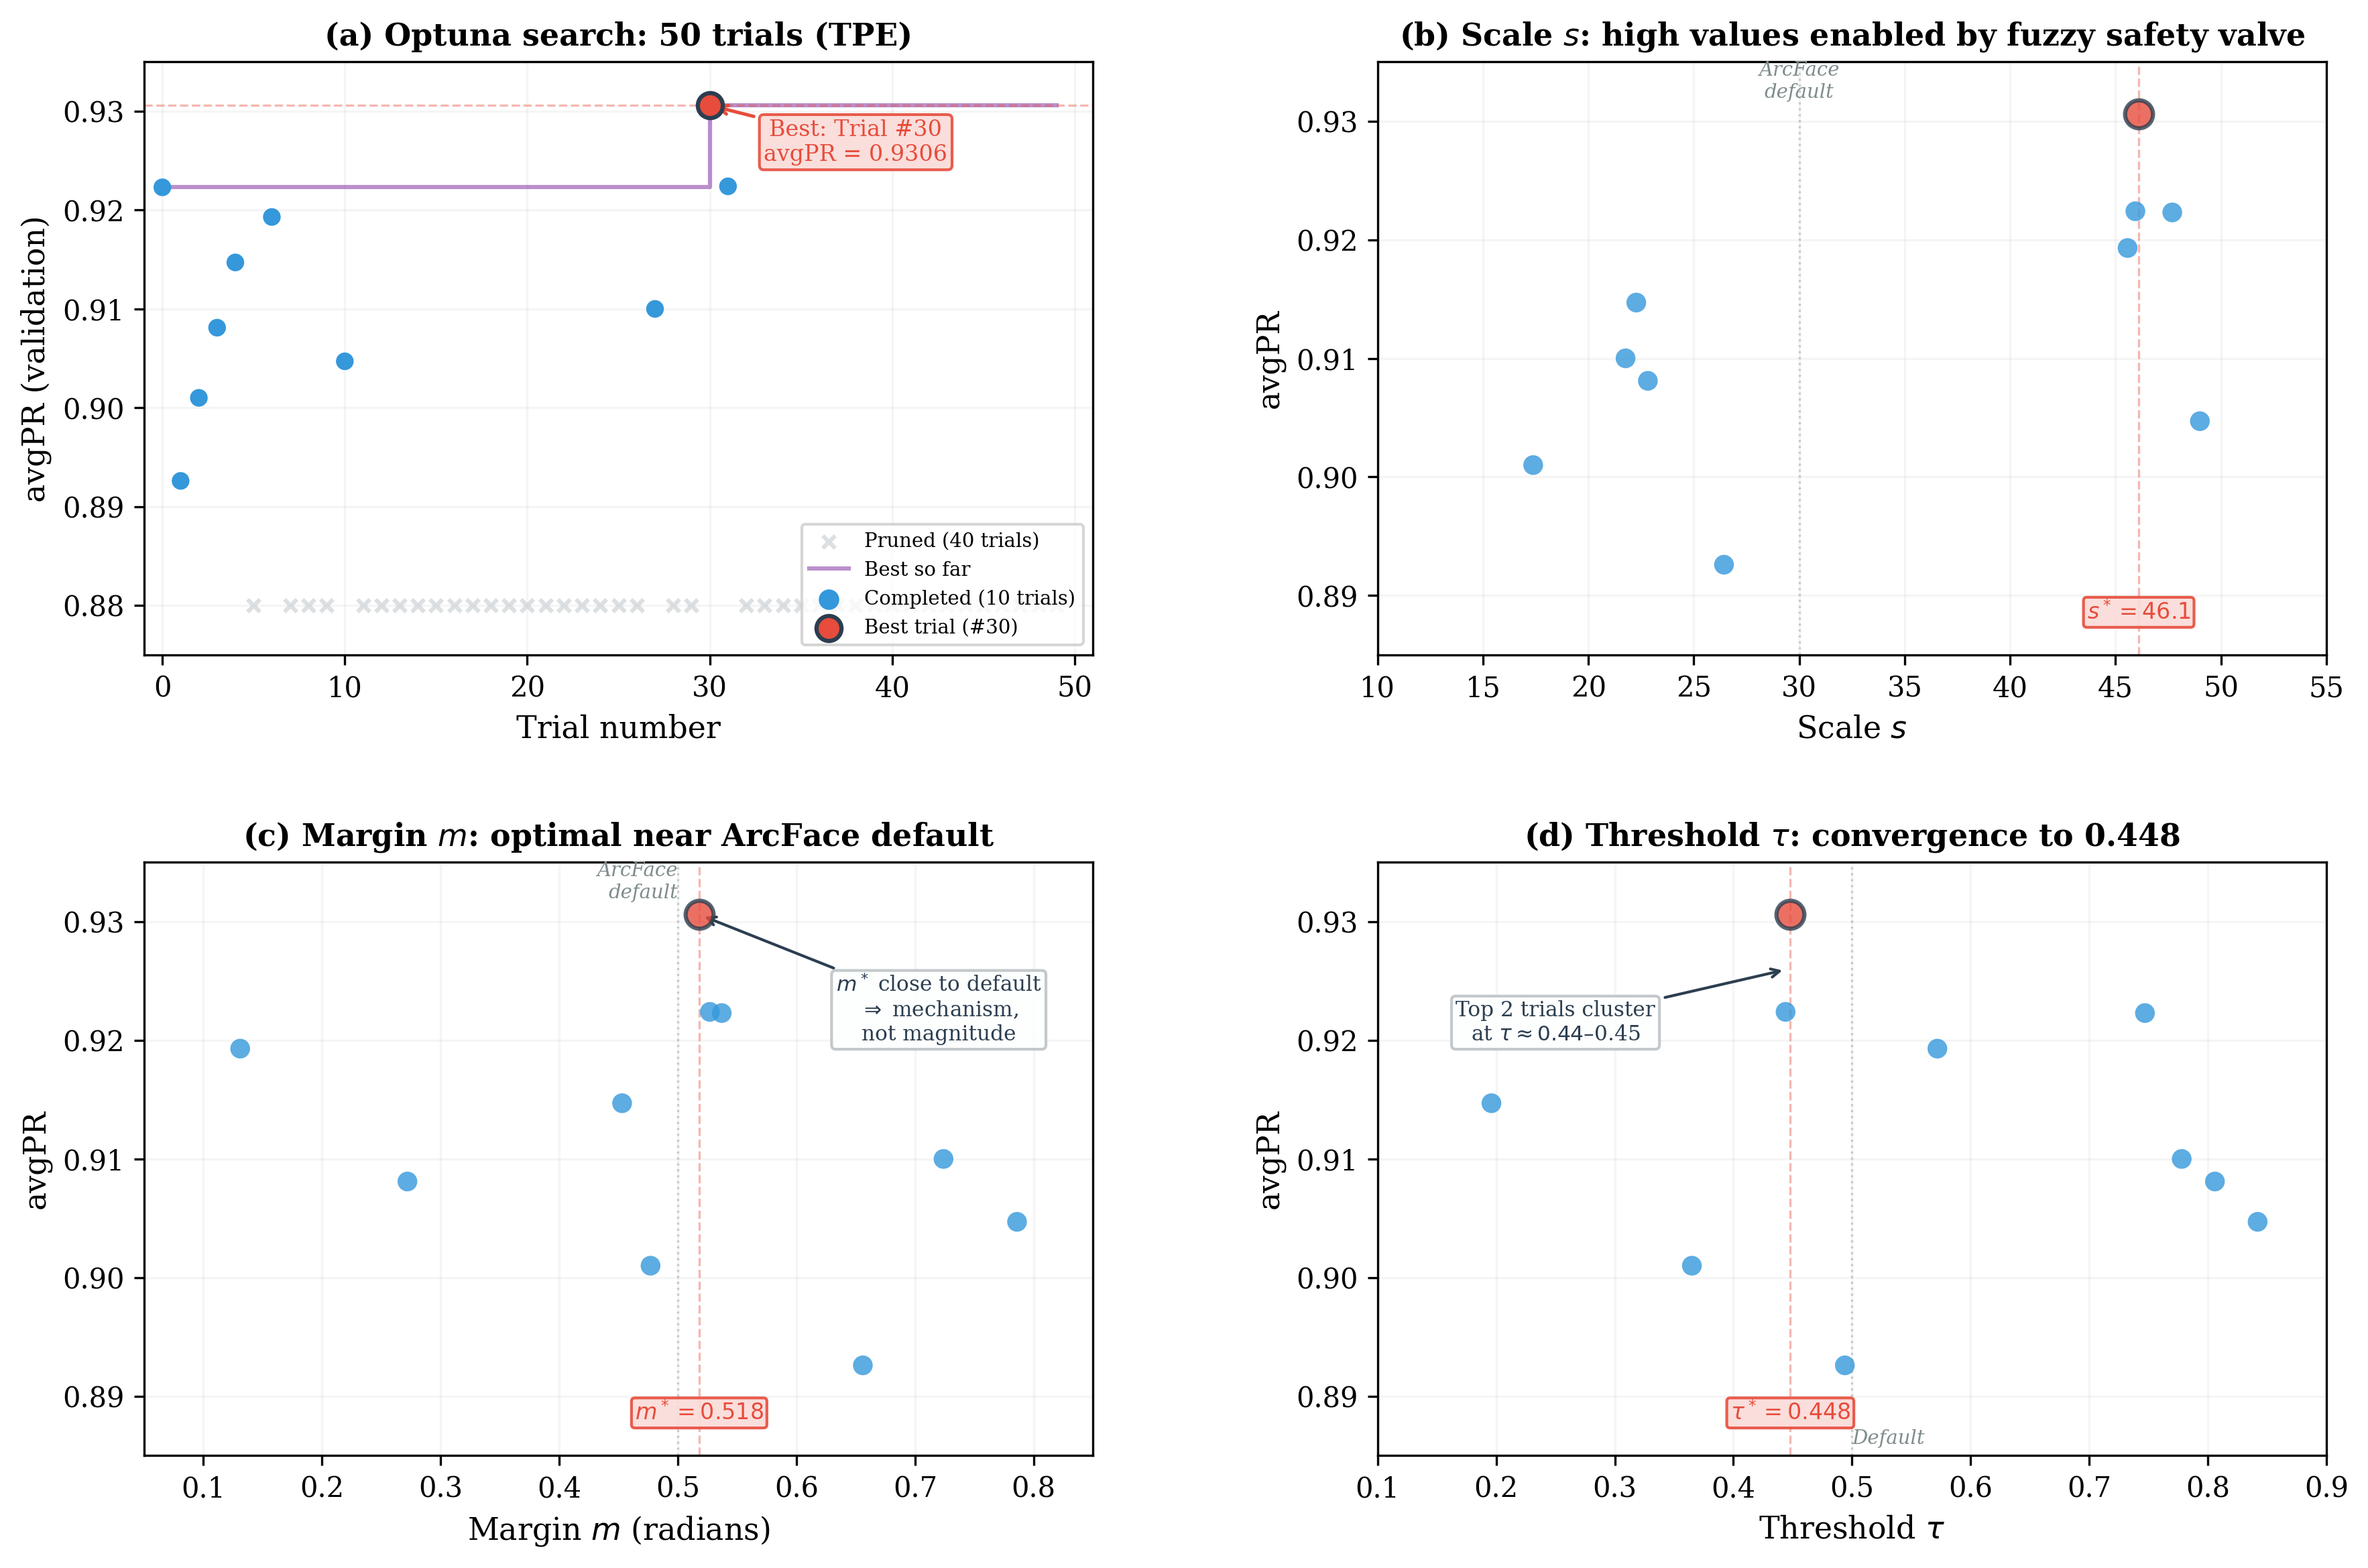
\includegraphics[width=\textwidth]{chapters/figures/optuna_search_fuzzyarcloss_v2.png}
\caption[Optuna hyperparameter search for FuzzyArcLoss~V2]{%
    Optuna Bayesian hyperparameter search (50 trials, TPE algorithm).
    \textbf{(a)}~Trial history: 10 of 50 trials completed
    (blue dots); 40 were pruned after epoch~20 (grey crosses).
    The purple step line tracks the best avgPR found so far;
    trial~\#30 (red) achieved the global optimum
    (avgPR $= 0.9306$).
    \textbf{(b)}~Scale $s$ vs avgPR: the top-performing trials
    cluster at $s \approx 45$--$48$, substantially above the
    ArcFace default ($s = 30$, grey line).
    The fuzzy membership safety valve enables these aggressive
    scales without training instability.
    \textbf{(c)}~Margin $m$ vs avgPR: the optimal
    $m^* = 0.518$ is close to the ArcFace default ($m = 0.5$),
    confirming that the modulation mechanism---not the raw margin
    magnitude---drives V2's advantage.
    \textbf{(d)}~Threshold $\tau$ vs avgPR: the top two trials
    converge to $\tau \approx 0.44$--$0.45$, defining the
    confidence boundary between the two membership regimes.}
\label{fig:optuna_search}
\end{figure}

\subsection{Training Protocol --- Methodological Decisions}
\label{sec:meth:pattern:training}

At the methodological level, the pattern classifier's training
protocol is fully characterised by three decisions:
(i)~the validation objective is the macro precision--recall mean
($\mathrm{avgPR}$, Equation~\ref{eq:avgpr_optuna}), chosen to weight
minority patterns equally;
(ii)~the model checkpoint that propagates downstream is the
$\mathrm{avgPR}$-best one rather than the last-epoch one, so that
performance reported in Chapter~\ref{ch:evaluation} reflects the
peak rather than the end of training; and
(iii)~all reported evaluation metrics use the \emph{margin-free
logits} (i.e., $s\cos\theta_k$ without the angular margin term),
because the margin is a training-time regulariser and not a
deployment-time decision rule.
The numerical training schedule that realises this protocol
(optimiser, learning-rate schedule, warmup formula, batch size,
augmentation pipeline, and the choice to disable MixUp/CutMix) is
reported in Section~\ref{sec:impl:pattern:training_protocol}.

\subsubsection{Pipeline Audit: Methodologically Significant Fixes}
\label{sec:meth:pattern:pipeline_audit}

The training protocol above was not chosen \emph{a priori}; it is the
end-state of a systematic audit of the pattern-classification pipeline
that identified twenty implementation issues whose correction raised
macro-F1 \emph{uniformly across all 18 loss-function variants} by
approximately 18~percentage points
(from $71$--$76$\,\% to $89$--$95$\,\% on single-run evaluation;
see Chapter~\ref{ch:usecase}, Section~\ref{sec:uc:pipeline_fixes}).
Ten of those fixes are methodologically significant in that they
constrain the design of \emph{any} fuzzy or angular-margin training
pipeline on small histopathological datasets; the remaining ten are
correctness-only code fixes documented in the public
repository.\footnote{\url{https://github.com/slima2/lchai}, directory
\texttt{Thesis/training/artefact1\_pattern\_classifier/}.}
Table~\ref{tab:pipeline_fixes} lists the ten methodologically
significant fixes, ordered roughly by impact.

\begin{table}[ht!]
\centering
\small
\caption{The ten methodologically significant fixes in the pattern
classifier pipeline audit.
Impact bands: \textbf{HIGH} ($\geq 5$\,pp macro-F1 gain when
isolated), \textbf{MEDIUM} ($1$--$5$\,pp).
All ten fixes affected every one of the 18 loss-function variants
equally; their uniformity is what justifies treating the post-audit
state as a \emph{fair shared baseline} rather than as differential
support for any one loss.}
\label{tab:pipeline_fixes}
\begin{tabular}{c l c}
\hline
\textbf{\#} & \textbf{Fix} & \textbf{Impact} \\
\hline
1  & 4-channel input: RGB $+$ tissue mask                & HIGH \\
2  & fp32 precision (not fp16)                            & HIGH \\
3  & Validation uses margin-free logits                   & HIGH \\
4  & Test evaluation uses margin-free logits              & HIGH \\
5  & Label mapping: \texttt{normalize\_key} + fallback    & HIGH \\
6  & Loss: FocalCE with $\alpha = $ class-balanced        & HIGH \\
7  & MixUp/CutMix disabled                                & MEDIUM \\
8  & Gradient clipping disabled                           & MEDIUM \\
9  & Train/test split: 80/20 (not 70/15/15)               & MEDIUM \\
10 & Model selection on $\mathrm{avgPR}$ (not val\_F1)    & MEDIUM \\
\hline
\end{tabular}
\end{table}

\paragraph{Why these are methodological, not engineering.}
Five of the fixes shape what a sound training pipeline for an angular
margin loss \emph{must} look like, regardless of dataset.
\textbf{(i)~4-channel input (\#1).}
Without an explicit binary tissue mask as a fourth channel, the model
must rediscover the foreground--background distinction from only 637
expert-annotated tiles; folding the mask in as a spatial prior
removes that burden and is responsible for an estimated $15$--$20$\,pp
of the audit's gain.
\textbf{(ii)~fp32 numerics (\#2).}
Mixed-precision (fp16) training silently corrupts gradients in
ArcFace-style losses because $\cos\theta$ and $\arccos$ involve small
numerical differences that fp16 rounds to zero;
fp32 is therefore not a runtime preference but a correctness
constraint.
\textbf{(iii)~Margin-free evaluation logits (\#3, \#4).}
The angular margin is a training-time regulariser that intentionally
penalises the correct class to widen the inter-class angular gap;
using margin-laden logits at evaluation time would suppress correct
predictions and report artificially low macro-F1 scores for every
margin-based variant in the benchmark.
\textbf{(iv)~MixUp disablement (\#7).}
MixUp interpolates images and one-hot labels linearly, but the angular
margin is applied per-sample to a \emph{single} integer class index;
linear blending of labels destroys this geometry, and the audit
confirmed that MixUp produced uniformly worse models across all 18
variants.
\textbf{(v)~$\mathrm{avgPR}$ model selection (\#10).}
Validation-F1 with class imbalance can over-reward a checkpoint that
sacrifices the minority cribriform/micropapillary classes;
$\mathrm{avgPR}$ (Equation~\ref{eq:avgpr_optuna}) weights all six
classes equally and is therefore the methodologically correct
selector.
The remaining five fixes (\#5, \#6, \#8, \#9, and details of \#3/\#4)
are listed in the table for completeness; together with the five
above they constitute the corrected baseline on which all
Chapter~\ref{ch:evaluation} comparisons rest.

The same five insights apply directly to any application of ArcFace,
CosFace, or SphereFace to small-dataset classification beyond
histopathology, and constitute a practical methodological contribution
of this thesis.


% ============================================================================
\section{Artefact 2: Pattern-Informed ABMIL for Mutation Prediction}
\label{sec:meth:mutation_prediction}
% ============================================================================

This section presents the methodology for the mutation prediction task, which constitutes the second artefact: Pattern-Informed Attention-Based Multiple Instance Learning (Pattern-Informed ABMIL).

\subsection{Task Formulation}
\label{sec:meth:mutation:task}

The mutation prediction task is formulated as a collection of independent binary classification problems, one per target gene $g \in \mathcal{G} = \{\textit{TP53},\allowbreak\, \textit{EGFR},\allowbreak\, \textit{KRAS},\allowbreak\, \textit{STK11},\allowbreak\, \textit{KEAP1},\allowbreak\, \textit{RBM10}\}$.
For each slide $s$ with tile set $\mathcal{T}_s$ and mutation label $Y_s^{(g)} \in \{0, 1\}$, the goal is to learn a function:
\begin{equation}
\label{eq:mutation_task}
f_g: \{\mathbf{h}_1, \mathbf{h}_2, \ldots, \mathbf{h}_{N_s}\} \mapsto \hat{Y}_s^{(g)} \in [0, 1],
\end{equation}
where $\mathbf{h}_i$ is the representation of tile $i$ (whose definition varies across experimental conditions).

\subsection{Tile-Level Representations Across Conditions}
\label{sec:meth:mutation:representations}

The six experimental conditions differ in how the tile-level representation $\mathbf{h}_i$ is constructed.
Let $\mathbf{x}_i \in \mathbb{R}^{512}$ be the CTransPath embedding and $\mathbf{p}_i \in \Delta^5$ the six-dimensional pattern probability vector (where $\Delta^5$ denotes the 5-simplex, i.e., $\sum_k p_{i,k} = 1$ and $p_{i,k} \geq 0$), both obtained from Artefact~1.
Let $\mathbf{o}_i \in \{0,1\}^6$ be the one-hot encoding of the predicted pattern class $\hat{y}_i = \arg\max_k p_{i,k}$.

\begin{table}[ht!]
\centering
\caption{Tile-level representation $\mathbf{h}_i$ for each experimental condition.}
\label{tab:tile_representations}
\begin{tabular}{c l l c}
\hline
\textbf{ID} & \textbf{Condition} & \textbf{Tile representation $\mathbf{h}_i$} & \textbf{Dim.} \\
\hline
B1 & XGBoost (floor baseline) & N/A (slide-level features) & 7 \\
B2 & ABMIL --- embeddings (ceiling baseline) & $\mathbf{h}_i = \mathbf{x}_i$ & 512 \\
B3 & ABMIL --- patterns & $\mathbf{h}_i = \mathbf{p}_i$ & 6 \\
PI-ABMIL  & PI-ABMIL (ours) & $\mathbf{h}_i = [\mathbf{x}_i \,\|\, \mathbf{p}_i]$ & 518 \\
A  & Ablation (one-hot) & $\mathbf{h}_i = [\mathbf{x}_i \,\|\, \mathbf{o}_i]$ & 518 \\
FC-MIL & FC-MIL (hybrid, ours) & $\mathbf{h}_i = (\mathbf{x}_i, \mathbf{p}_i)$ (dual pathway) & 512+6 \\
\hline
\end{tabular}
\end{table}

\textbf{Two baselines: floor and ceiling.}
Two baselines frame the evaluation from below and above.
\textbf{B1 (floor baseline)} uses XGBoost on seven slide-level pattern
features (six pattern percentages $+$ entropy), establishing the
\emph{minimum} performance achievable from pattern information alone
without deep learning, tile-level representations, or attention
mechanisms.
\textbf{B2 (ceiling baseline)} uses ABMIL on CTransPath embeddings
alone, with the same attention architecture, pretrained encoder, and
training protocol as the proposed methods (PI-ABMIL, FC-MIL),
differing only in the absence of explicit pattern information.
B2 therefore establishes the \emph{maximum} performance achievable
from visual embeddings without domain knowledge; any pattern-informed
method must match or exceed B2 to justify the added complexity.
By holding everything else constant, the delta between any
pattern-informed condition and B2 isolates the \emph{incremental value}
of injecting histological pattern knowledge into the pipeline.

\textbf{The key comparison} is therefore between PI-ABMIL and B2.
If PI-ABMIL outperforms B2, the fuzzy pattern probabilities contribute information beyond what the CTransPath embeddings encode implicitly.
The comparison between PI-ABMIL and A tests whether the continuous (fuzzy) representation $\mathbf{p}_i$ is more informative than the discrete (crisp) representation $\mathbf{o}_i$.

\subsection{Attention-Based MIL Architecture}
\label{sec:meth:mutation:abmil}

For conditions B2, B3, PI-ABMIL, and A, the ABMIL architecture~\cite{ilse2018attention} consists of three modules: a tile-level transformation, an attention mechanism, and a slide-level classifier.

\subsubsection{Tile-Level Transformation}

Each tile representation is projected through a two-layer feedforward network:
\begin{equation}
\label{eq:tile_transform}
\mathbf{h}_i' = \text{ReLU}(\mathbf{W}_2 \cdot \text{ReLU}(\mathbf{W}_1 \mathbf{h}_i + \mathbf{b}_1) + \mathbf{b}_2) \in \mathbb{R}^{L},
\end{equation}
where $L = 256$ is the hidden dimension.
Dropout~\cite{srivastava2014dropout} with $p = 0.25$ is applied after each ReLU activation.

\subsubsection{Gated Attention Mechanism}

The attention weight for tile $i$ is computed using the gated attention formulation~\cite{ilse2018attention,lu2021data}:
\begin{equation}
\label{eq:gated_attn}
a_i = \frac{\exp\left(\mathbf{w}^\top \left(\tanh(\mathbf{V} \mathbf{h}_i') \odot \sigma(\mathbf{U} \mathbf{h}_i')\right)\right)}{\sum_{j=1}^{N_s} \exp\left(\mathbf{w}^\top \left(\tanh(\mathbf{V} \mathbf{h}_j') \odot \sigma(\mathbf{U} \mathbf{h}_j')\right)\right)},
\end{equation}
where $\mathbf{V}, \mathbf{U} \in \mathbb{R}^{128 \times L}$ are the attention and gating transformation matrices, $\mathbf{w} \in \mathbb{R}^{128}$ is the attention vector, $\sigma$ denotes the sigmoid function, and $\odot$ is element-wise multiplication.
The gating mechanism allows the network to suppress irrelevant tiles (e.g., normal tissue, necrosis, artefacts) more aggressively than standard $\tanh$-only attention.

\subsubsection{Slide-Level Aggregation and Classification}

The slide-level representation is the attention-weighted sum of the transformed tile features:
\begin{equation}
\label{eq:slide_repr}
\mathbf{z}_s = \sum_{i=1}^{N_s} a_i \, \mathbf{h}_i' \in \mathbb{R}^{L}.
\end{equation}

The mutation prediction for gene $g$ is obtained through a linear classifier:
\begin{equation}
\label{eq:mutation_pred}
\hat{Y}_s^{(g)} = \sigma\left(\mathbf{w}_g^\top \mathbf{z}_s + b_g\right),
\end{equation}
where $\mathbf{w}_g \in \mathbb{R}^L$ and $b_g \in \mathbb{R}$ are gene-specific parameters.
A separate ABMIL model is trained for each gene, following the standard practice in the field~\cite{coudray2018classification,saldanha2023npj}.

\subsubsection{Training Objective}

The ABMIL model is trained to minimise the binary cross-entropy loss:
\begin{equation}
\label{eq:bce}
\mathcal{L}_{\text{BCE}}^{(g)} = -\frac{1}{|\mathcal{S}|} \sum_{s \in \mathcal{S}} \left[Y_s^{(g)} \log \hat{Y}_s^{(g)} + (1 - Y_s^{(g)}) \log(1 - \hat{Y}_s^{(g)})\right],
\end{equation}
where $\mathcal{S}$ is the set of slides in the training fold.

Figure~\ref{fig:abmil_architecture} provides a block diagram of the
complete ABMIL architecture, showing the data flow from tile
representations through the three modules and the loss function,
with equation references and input dimensions for each experimental
condition.

\begin{figure}[ht!]
\centering
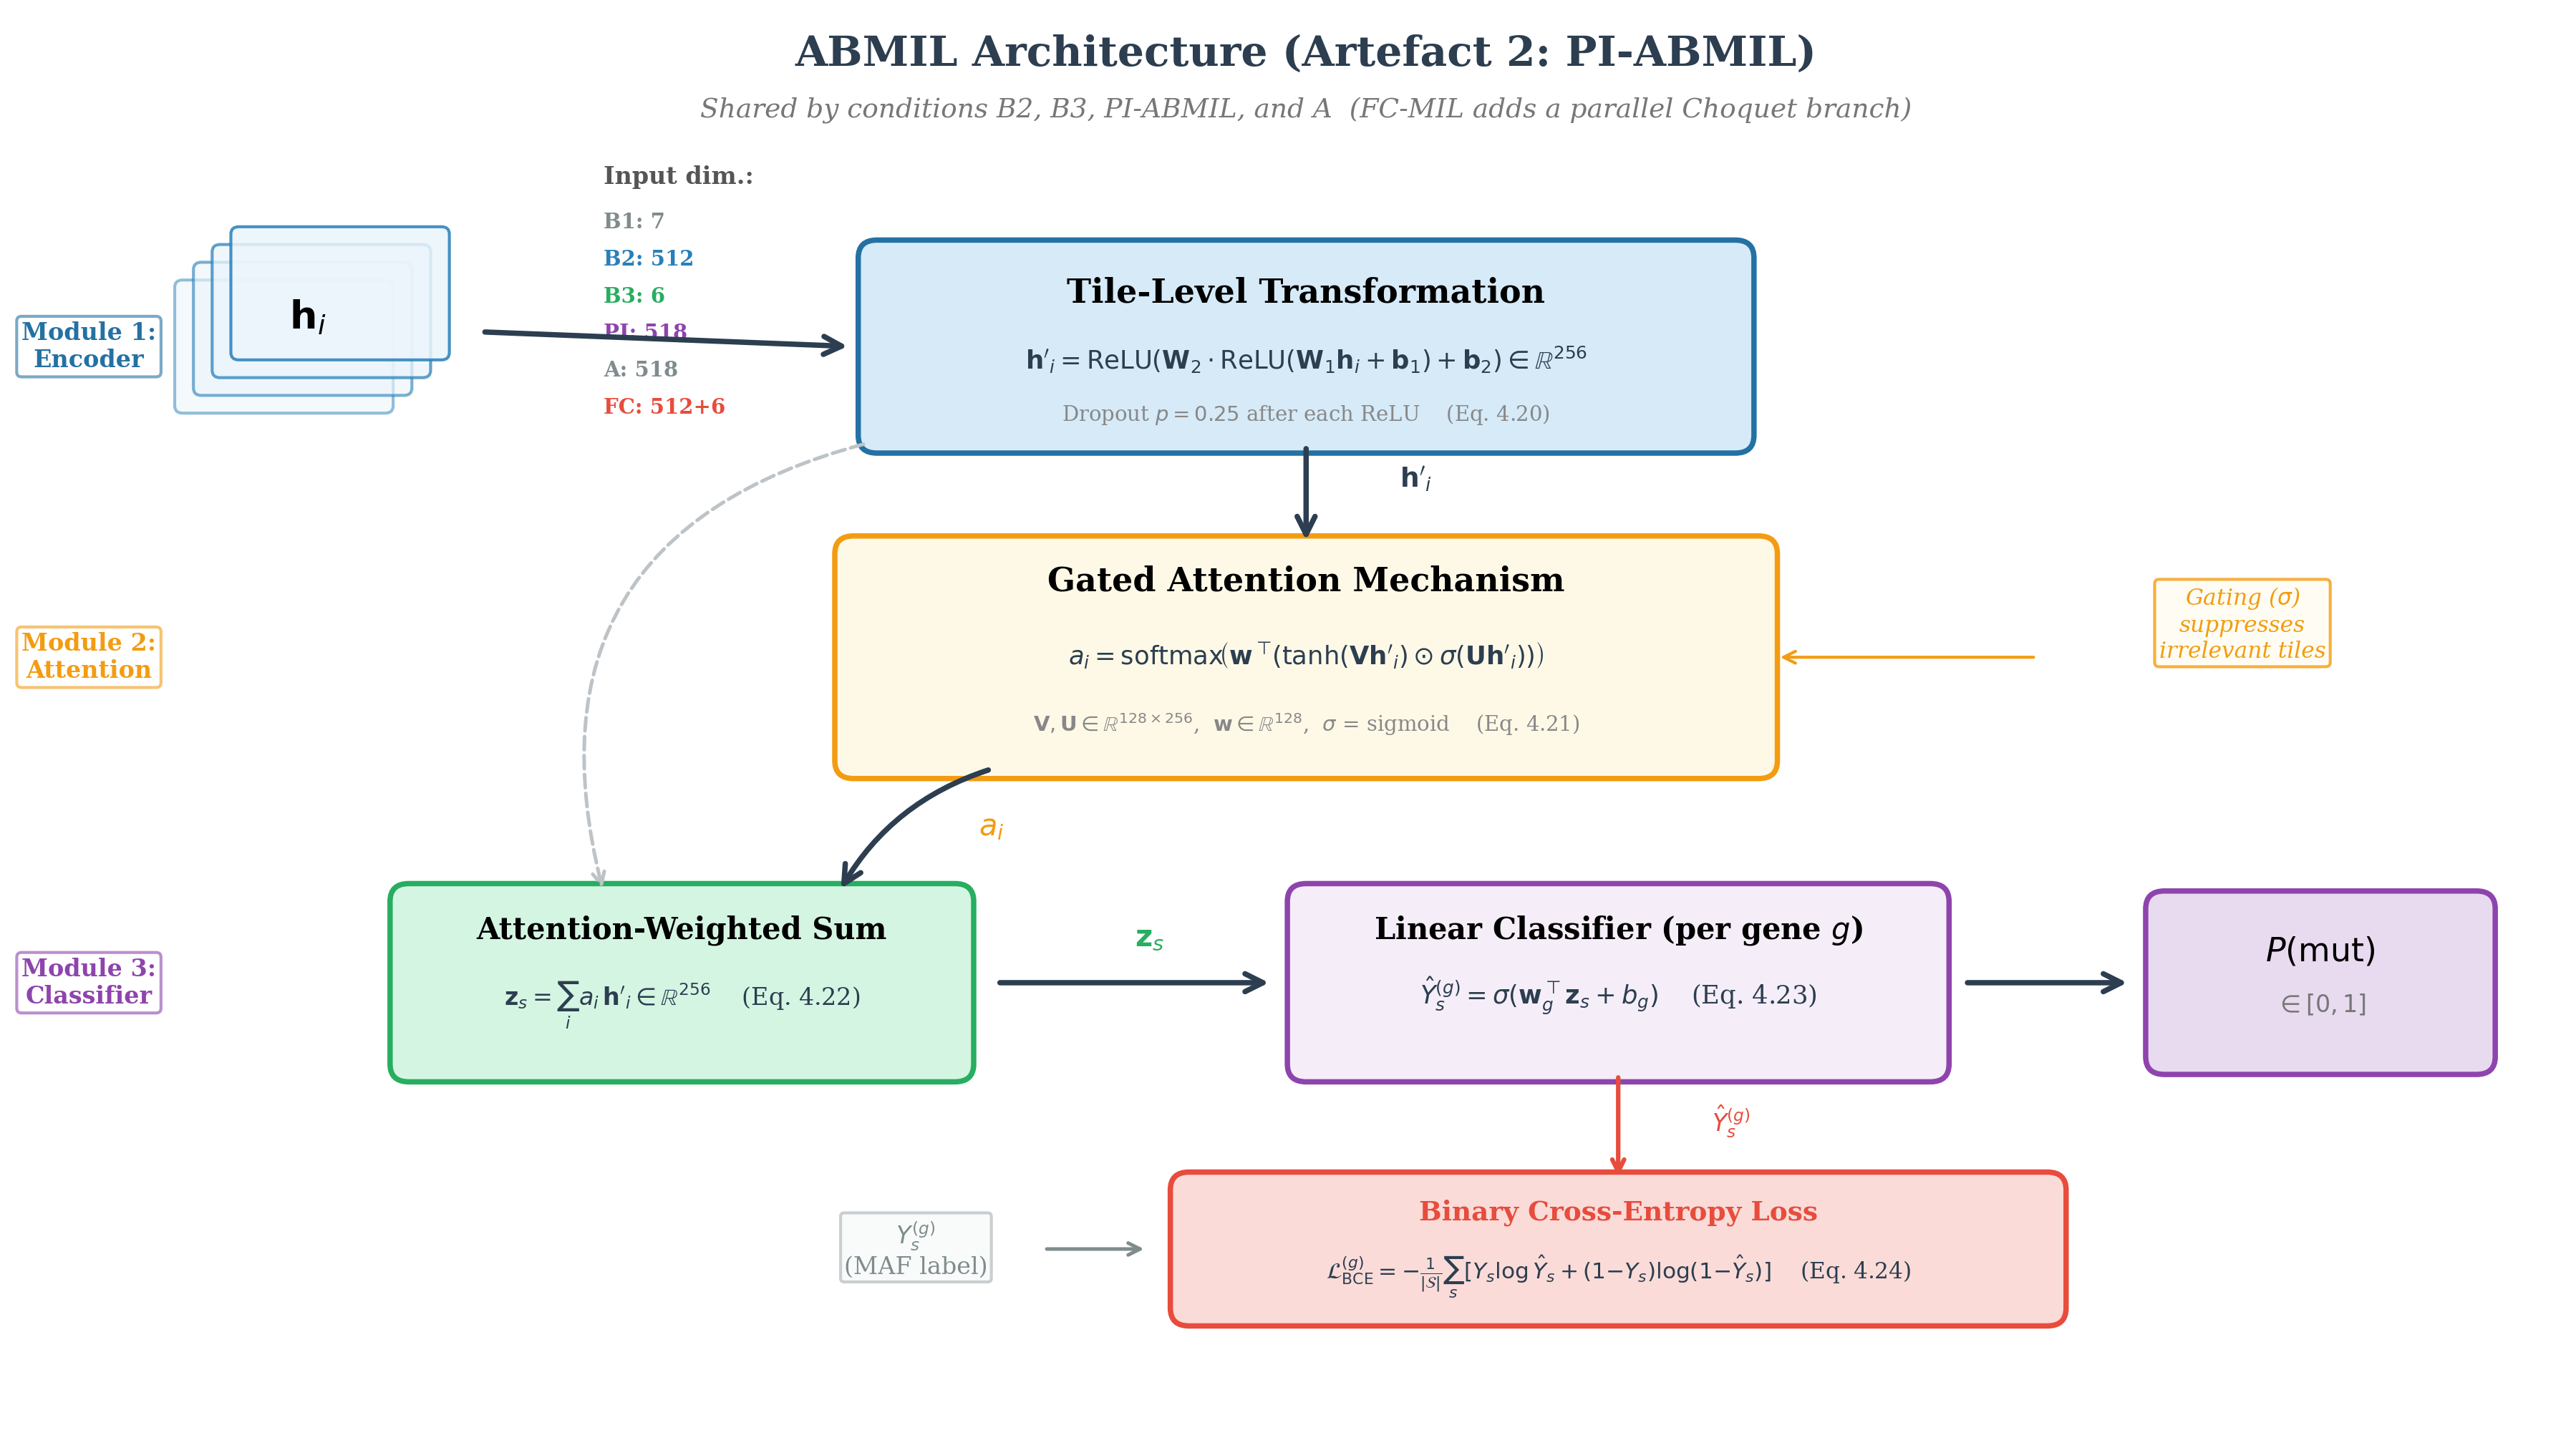
\includegraphics[width=\textwidth]{chapters/figures/abmil_architecture.png}
\caption[ABMIL architecture for mutation prediction]{%
    Block diagram of the ABMIL architecture (Artefact~2)
    shared by conditions B2, B3, PI-ABMIL, and~A.
    \textbf{Module~1 (Encoder):} A two-layer feedforward network
    projects the condition-specific tile representation
    $\mathbf{h}_i$ (dim.\ 7--518) to a hidden space
    $\mathbf{h}'_i \in \mathbb{R}^{256}$
    (Eq.~\ref{eq:tile_transform}).
    \textbf{Module~2 (Gated Attention):} Sigmoid gating
    suppresses irrelevant tiles (necrosis, artefacts) and
    computes per-tile importance weights $a_i$
    (Eq.~\ref{eq:gated_attn}).
    \textbf{Module~3 (Classifier):} The attention-weighted sum
    $\mathbf{z}_s$ (Eq.~\ref{eq:slide_repr}) is passed through
    a gene-specific linear head producing $P(\mathrm{mut})$
    (Eq.~\ref{eq:mutation_pred}), trained with binary
    cross-entropy (Eq.~\ref{eq:bce}).
    FC-MIL adds a parallel Choquet branch (not shown;
    see Section~\ref{sec:meth:choquet_mil}).
    Input dimensions per condition are listed in the top-left
    (Table~\ref{tab:tile_representations}).}
\label{fig:abmil_architecture}
\end{figure}


\subsection{Floor Baseline B1: XGBoost on Slide-Level Pattern Features}
\label{sec:meth:mutation:xgboost}

Condition B1 serves as a \emph{floor baseline}: a non-deep-learning
method that establishes the minimum performance achievable from
pattern information alone, without attention mechanisms or
tile-level representations.
For each slide $s$, a seven-dimensional feature vector is computed from the tile-level pattern predictions:
\begin{equation}
\label{eq:xgboost_features}
\mathbf{f}_s = \left[\text{frac}_1, \text{frac}_2, \ldots, \text{frac}_6, H_s\right] \in \mathbb{R}^7,
\end{equation}
where $\text{frac}_k = |\{i : \hat{y}_i = k\}| / N_s$ is the fraction of tiles assigned to pattern $k$, and $H_s = -\sum_{k=1}^{6} \text{frac}_k \log(\text{frac}_k + \epsilon)$ is the Shannon entropy of the pattern distribution, measuring intra-tumoral heterogeneity.

An XGBoost gradient-boosted tree classifier~\cite{chen2016xgboost} is trained on these seven features.
XGBoost is chosen for its robustness to small sample sizes, built-in regularisation, and compatibility with SHAP~\cite{lundberg2017shap} for feature attribution.

\textbf{Rationale.}
Converting locally ambiguous tile predictions into a global distributional
representation yields two advantages:
(i)~it is robust to individual tile labelling errors, since the mutation
genotype is better reflected by global architectural composition than by
any single microscopic region~\cite{coudray2018classification}; and
(ii)~it produces a fixed-dimensional case representation regardless of
slide size (5{,}000--80{,}000 tiles), enabling direct comparison across
the heterogeneous TCGA-LUAD cohort~\cite{tcga2014luad}.
 

% ============================================================================
\section{Artefact 3: Fuzzy Choquet MIL}
\label{sec:meth:choquet_mil}
% ============================================================================

The Fuzzy Choquet MIL architecture replaces the attention-weighted aggregation of standard ABMIL with a Choquet integral operating on tile-level fuzzy pattern memberships.
This section presents its mathematical formulation.

\subsection{Motivation}
\label{sec:meth:choquet:motivation}

The standard ABMIL attention mechanism (Equation~\ref{eq:gated_attn}) learns which \emph{tiles} are important but treats each tile's pattern memberships independently.
It cannot model interactions between patterns: for example, the co-occurrence of solid and micropapillary morphology in the same tumour may predict TP53 mutation more strongly than either pattern alone, but ABMIL has no mechanism to capture this superadditive effect.

The Choquet integral~\cite{choquet1954theory,grabisch2009aggregation} provides exactly this capability.
By operating on the six-dimensional fuzzy membership vector with a learned fuzzy measure, it aggregates pattern contributions while accounting for pairwise (and higher-order) interactions between patterns.

\subsection{Architecture}
\label{sec:meth:choquet:architecture}

The Fuzzy Choquet MIL pipeline follows a \emph{dual-pathway} architecture
that processes embeddings and pattern memberships through separate branches
before merging them for classification.

\subsubsection{Embedding Pathway (Shared with ABMIL)}

The CTransPath embedding $\mathbf{x}_i \in \mathbb{R}^{512}$ of each tile
is projected through the same encoder--attention architecture used in
Artefact~2:
\begin{equation}
\label{eq:choquet_emb_path}
\mathbf{z}_{\text{attn}} = \sum_{i=1}^{N_s} \alpha_i \, \text{Encoder}(\mathbf{x}_i) \in \mathbb{R}^{256},
\end{equation}
where $\text{Encoder}$ is a two-layer feedforward network
($512 \to 256$, LayerNorm, ReLU, Dropout) and $\alpha_i$ are gated
attention weights (Equation~\ref{eq:gated_attn}).
This pathway captures the same visual features as condition~B2.

\subsubsection{Choquet Pathway (Pattern Interactions)}

In parallel, the tile-level fuzzy membership vectors
$\{\mathbf{p}_1, \ldots, \mathbf{p}_{N_s}\}$ are passed through the
discrete Choquet integral with a learned 2-additive fuzzy measure~\cite{grabisch1997kapprox} $g$.
Following Section~\ref{sec:bg:choquet:secondorder}, the fuzzy measure is
parameterised by Shapley values $\{\phi_k\}_{k=1}^{6}$ and pairwise
interaction indices $\{I_{jk}\}_{j < k}$:
\begin{equation}
\label{eq:fuzzy_measure_method}
g(A) = \sum_{k \in A} \phi_k + \sum_{\{j,k\} \subseteq A} I_{jk}, \quad A \subseteq \{1, \ldots, 6\}.
\end{equation}

The Shapley values~\cite{shapley1953value} are constrained to be non-negative and sum to~1 via a
softmax parameterisation:
\begin{equation}
\label{eq:shapley_param}
\phi_k = \frac{e^{\psi_k}}{\sum_{l=1}^{6} e^{\psi_l}}, \quad \psi_k \in \mathbb{R} \text{ (unconstrained)}.
\end{equation}

The interaction indices are unconstrained but regularised toward zero to
encourage sparsity:
\begin{equation}
\label{eq:interaction_reg}
\mathcal{R}_{\text{int}} = \lambda_I \sum_{j < k} |I_{jk}|,
\end{equation}
with $\lambda_I = 0.01$.

The standard discrete Choquet integral
$\mathcal{C}_g(\bar{\mathbf{p}}_s) \in \mathbb{R}$ collapses the
six fuzzy memberships into a single scalar.
For the FC-MIL aggregation pathway, however, we retain the
\emph{rank-ordered Choquet differential terms} as a vector
$\mathbf{c}_s \in \mathbb{R}^6$ with components
$c_{s,(i)} = (\bar{p}_{\sigma(i)} - \bar{p}_{\sigma(i-1)})\,g(A_i)$,
where $\sigma$ is the slide-level sort permutation and
$A_i = \{\sigma(i), \ldots, \sigma(6)\}$.
The classical scalar Choquet output equals
$\mathbf{1}^\top \mathbf{c}_s$, so $\mathbf{c}_s$ is a strict
decomposition of the integral that preserves per-rank pattern
identity for the merge step.
The concrete differentiable PyTorch routine that computes this
decomposition is given in Section~\ref{sec:impl:choquet:module}.

\subsubsection{Merge and Classification}

The two pathway outputs are concatenated and projected to the hidden
dimension before classification:
\begin{equation}
\label{eq:choquet_merge}
\mathbf{z}_s = \text{ReLU}\!\left(\mathbf{W}_{\text{proj}}
\left[\mathbf{c}_s \,\|\, \mathbf{z}_{\text{attn}}\right] + \mathbf{b}_{\text{proj}}\right)
\in \mathbb{R}^{256},
\end{equation}
where $\mathbf{W}_{\text{proj}} \in \mathbb{R}^{256 \times 262}$.
The mutation prediction is:
\begin{equation}
\label{eq:choquet_classifier}
\hat{Y}_s^{(g)} = \sigma\left(\mathbf{w}_g^\top \mathbf{z}_s + b_g\right).
\end{equation}

This dual-pathway design means the Choquet branch contributes
\emph{interpretable pattern interaction information} alongside the
embedding-based attention, rather than replacing it.
The fuzzy measure's 21~parameters (6~Shapley values + 15~interaction
indices) remain intrinsically interpretable even though the full model
shares the embedding encoder with ABMIL.

Figure~\ref{fig:fcmil_architecture} illustrates the complete
dual-pathway architecture, showing the provenance of both input
streams from Artefact~1 and the data flow through the embedding
and Choquet branches to the merged classifier.

\begin{figure}[ht!]
\centering
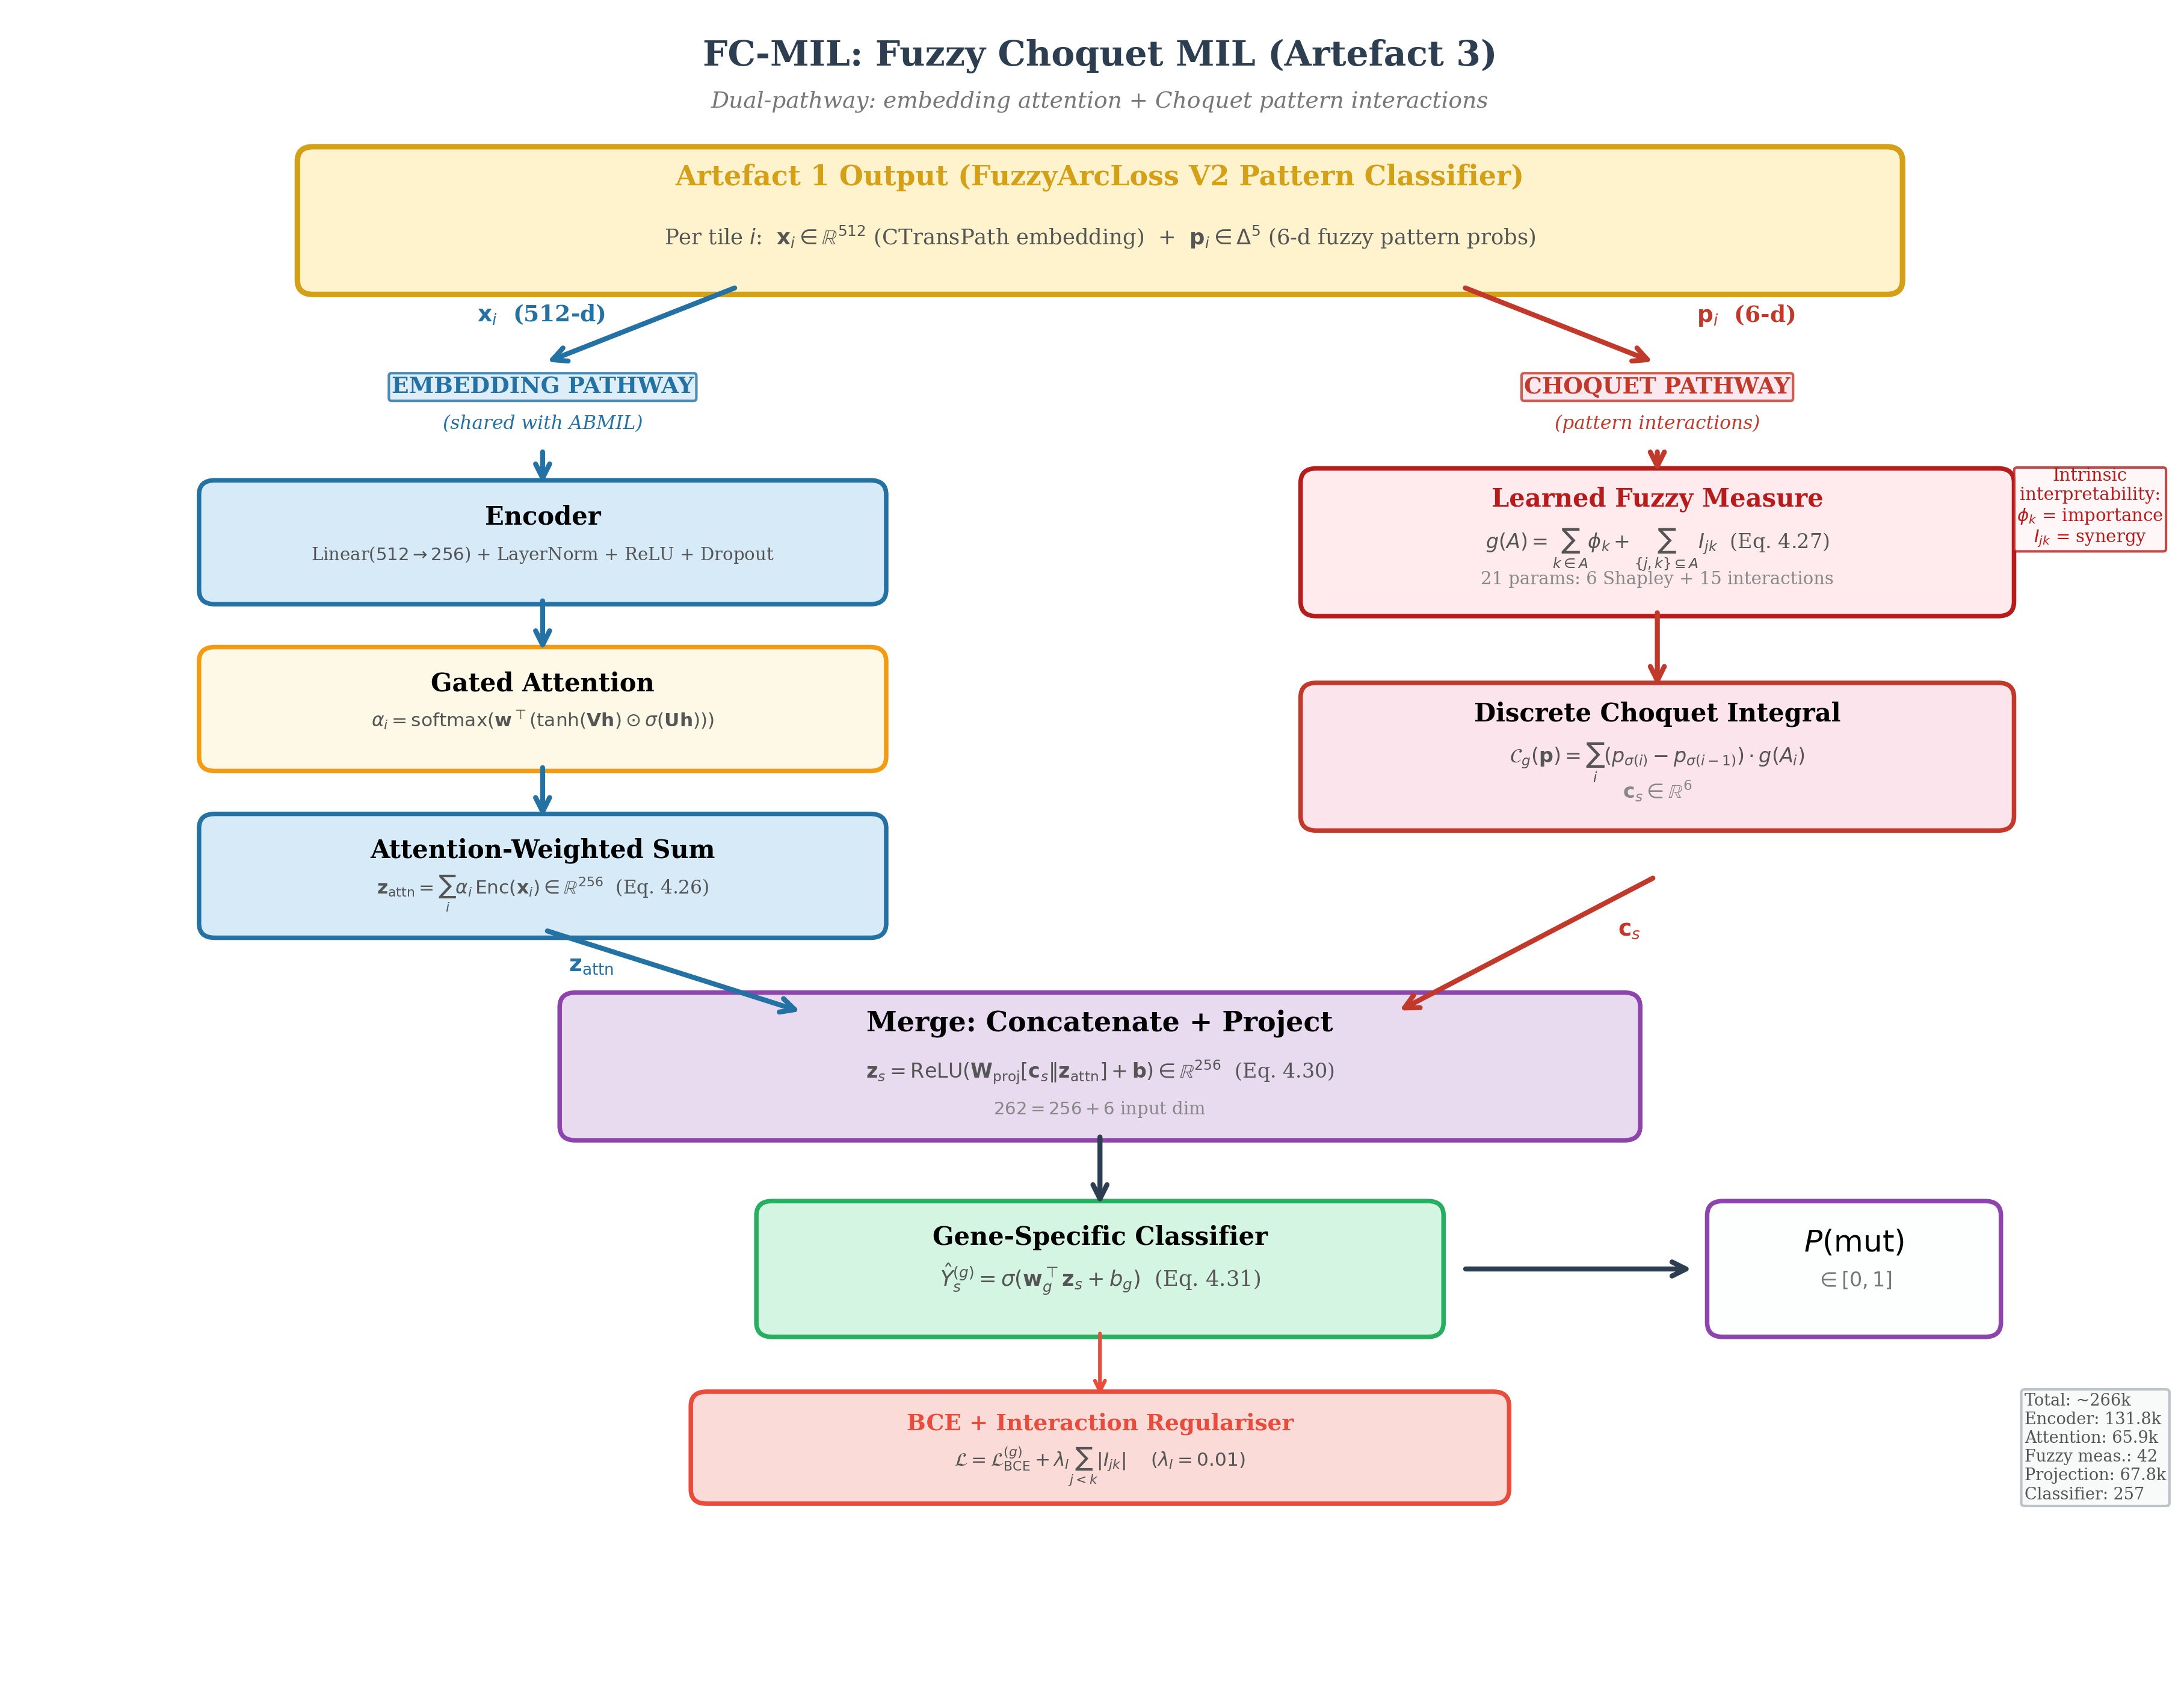
\includegraphics[width=\textwidth]{chapters/figures/fcmil_architecture.png}
\caption[FC-MIL dual-pathway architecture]{%
    FC-MIL (Fuzzy Choquet MIL) dual-pathway architecture (Artefact~3).
    \textbf{Top}: Both input streams originate from Artefact~1
    (FuzzyArcLoss~V2 pattern classifier): the 512-d CTransPath
    embedding $\mathbf{x}_i$ and the 6-d fuzzy pattern probability
    vector $\mathbf{p}_i \in \Delta^5$.
    The pattern probabilities are \emph{not} derived from the focal
    or label-smoothing loss---those are training objectives of
    Artefact~1; $\mathbf{p}_i$ is the softmax output of the frozen
    classifier at inference time.
    \textbf{Left (blue)}: Embedding pathway shared with ABMIL---encoder,
    gated attention, and attention-weighted sum producing
    $\mathbf{z}_{\mathrm{attn}} \in \mathbb{R}^{256}$
    (Eq.~\ref{eq:choquet_emb_path}).
    \textbf{Right (red)}: Choquet pathway---a learned 2-additive fuzzy
    measure with 21 interpretable parameters aggregates the pattern
    vectors via the discrete Choquet integral to produce
    $\mathbf{c}_s \in \mathbb{R}^6$
    (Eq.~\ref{eq:fuzzy_measure_method}).
    \textbf{Bottom}: The two pathway outputs are concatenated
    ($262 = 256 + 6$) and projected to $\mathbb{R}^{256}$
    (Eq.~\ref{eq:choquet_merge}) before gene-specific classification
    (Eq.~\ref{eq:choquet_classifier}).
    Total model: $\sim$266{,}000 parameters; the interpretable
    fuzzy measure accounts for only 21 of these
    (6 Shapley values + 15 pairwise interaction indices under the
    2-additive approximation~\cite{grabisch1997kapprox}).}
\label{fig:fcmil_architecture}
\end{figure}

\subsection{Parameter Count and Feasibility}
\label{sec:meth:choquet:params}

At the methodological level, the relevant parameter contrast between
the two MIL architectures is between the \emph{interpretable} fuzzy
measure (21 parameters) and the \emph{opaque} embedding-pathway
capacity ($\sim$200k parameters), not the per-layer breakdown.
Concretely:
\begin{itemize}
    \item PI-ABMIL totals $\sim$200{,}000 parameters, all in the
    embedding pathway and the binary classification head.
    \item FC-MIL totals $\sim$266{,}000 parameters; of these, only
    \textbf{21} are interpretable (the 2-additive fuzzy measure with
    6~Shapley values plus 15~pairwise interaction indices), and the
    remaining $\sim$266{,}000 are dominated by the merge-projection
    layer that fuses the embedding pathway and the Choquet branch.
\end{itemize}
The full per-layer breakdown (encoder, gated attention, Choquet
scale, merge projection, classifier head) is reported in
Table~\ref{tab:hyper_choquet2} of
Chapter~\ref{ch:implementation}.

Although FC-MIL is approximately 33\% larger than ABMIL overall
($\sim$266{,}000 vs $\sim$200{,}000 parameters), the additional
capacity serves the merge projection layer ($262 \to 256$), not
the interpretable component.
The fuzzy measure itself requires only 21 learnable
parameters---the minimum needed to capture singleton pattern
importance (6~Shapley values) and pairwise interactions
(15~indices) for six histological classes under the 2-additive
approximation~\cite{grabisch1997kapprox}.
This parsimony of the interpretable component is a deliberate
design feature: it ensures that the learned Shapley values and
interaction indices are sufficiently constrained to be meaningfully
interpretable, rather than overfitting to noise in the limited
training set ($\sim$687 slides).
A general (unconstrained) fuzzy measure over $n = 6$ sources would
require $2^n - 2 = 62$ parameters, tripling the interpretable
parameter count and making the individual Shapley contributions
harder to isolate.
The embedding pathway is shared with ABMIL to ensure that any
performance difference between conditions PI-ABMIL and FC-MIL is attributable to
the aggregation mechanism (concatenation vs Choquet integral), not to
differences in model capacity.

\subsection{Training Objective}
\label{sec:meth:choquet:training}

The Fuzzy Choquet MIL is trained with binary cross-entropy plus the
interaction regulariser and a soft monotonicity penalty
$\mathcal{R}_{\text{mono}}$ that enforces
$g(A) \leq g(B)$ for $A \subseteq B$ (a property the 2-additive
parameterisation does not satisfy automatically):
\begin{equation}
\label{eq:choquet_loss}
\mathcal{L}_{\text{Choquet}} = \mathcal{L}_{\text{BCE}}^{(g)}
+ \mathcal{R}_{\text{int}}
+ \mathcal{R}_{\text{mono}}.
\end{equation}
The explicit form of $\mathcal{R}_{\text{mono}}$, the strength
coefficient $\lambda_M$, and the Monte-Carlo subset-pair sampling
used to evaluate it efficiently are deferred to
Section~\ref{sec:impl:choquet:monotonicity}.

\textbf{Interpretability by construction.}
Unlike post-hoc explanation methods (SHAP~\cite{lundberg2017shap}, attention maps), the Choquet integral provides built-in interpretability through its learned parameters:
\begin{itemize}
    \item The Shapley value $\phi_k$ quantifies the marginal contribution of pattern $k$ to the fuzzy measure.
    Because the softmax parameterisation (Equation~\ref{eq:shapley_param}) ensures $\sum_k \phi_k = 1$, the uniform baseline is $\phi_k = 1/6 \approx 0.167$.
    Values substantially above $1/6$ indicate that the model considers pattern $k$ disproportionately important for the aggregation; values near $1/6$ for \emph{all} patterns indicate no learned pattern preference, meaning the Choquet integral approximates a simple average.
    \item The interaction index $I_{jk}$ indicates whether the co-occurrence of patterns $j$ and $k$ is synergistic ($I_{jk} > 0$) or redundant ($I_{jk} < 0$).
    Due to the $L_1$ regulariser (Equation~\ref{eq:interaction_reg}), learned indices are typically small ($|I_{jk}| \sim 0.01\text{--}0.05$); this is expected and does not indicate irrelevance.
    Even small interaction indices modify the fuzzy measure at the pair level, altering how pattern combinations are weighted in the Choquet aggregation.
\end{itemize}

\textbf{Causal chain to $P(\text{mut})$.}
The Shapley values and interaction indices are \emph{not} in the same units as $P(\text{mut})$ and do not add to or subtract from it directly.
The relationship is:
\begin{quote}
pattern scores $\mathbf{p}_i$ $\;\to\;$ Choquet integral (shaped by $\phi_k$, $I_{jk}$) $\;\to\;$ $\mathbf{c}_s \in \mathbb{R}^6$ $\;\to\;$ concat with $\mathbf{z}_{\text{attn}}$ $\;\to\;$ projection $\;\to\;$ $\sigma(\cdot)$ $\;\to\;$ $P(\text{mut})$.
\end{quote}
A near-uniform Shapley profile with small interaction indices means the Choquet branch contributes a pattern-averaged signal, and the discriminative power comes primarily from the shared embedding pathway via $\mathbf{z}_{\text{attn}}$.
Conversely, if specific patterns deviate substantially from $1/6$ or strong interactions emerge, the Choquet branch encodes pattern-specific information that complements the embedding attention.

Figure~\ref{fig:choquet_interpretability} illustrates these concepts
using \textbf{real learned values} from the trained FC-MIL checkpoints
(Chapter~\ref{ch:evaluation}), contrasting two genes with
qualitatively different interaction structures.

\textbf{KRAS: uniform singletons, structured interactions.}
Panel~(a) shows that both KRAS and RBM10 have near-uniform singleton
Shapley values ($\phi_k \approx 0.165$--$0.170$, deviations $< 0.5\%$
from $1/6$), classified as ``Uniform'' by the fuzzy profile scale
(Section~\ref{sec:meth:interp:fuzzy_labels}).
This means no single pattern dominates the aggregation for either
gene.
However, the interaction heatmaps reveal a stark contrast.
For KRAS (panel~b), the lepidic$\times$solid pair has
$I = +0.032$, classified by the trapezoidal fuzzy scale as
``Moderate~$\uparrow$'' (supra-additive interaction: their
co-occurrence is more predictive than either pattern alone).
Solid$\times$acinar ($I = +0.025$) also shows ``Moderate~$\uparrow$.''
In contrast, micropapillary$\times$cribriform ($I = -0.025$)
is classified ``Moderate~$\downarrow$'' (sub-additive: these
patterns carry overlapping information).

\textbf{RBM10: uniform singletons, flat interactions.}
For RBM10 (panel~c), all interaction indices are near zero
(max $|I| = 0.008$), an order of magnitude smaller than the KRAS
values.
The model has learned an effectively \emph{flat} measure---the
Choquet integral reduces to a simple average, confirming that
no pattern or pattern combination carries discriminative signal for
this RNA splicing factor gene.

\textbf{Key observation.}
The insight lies not in the singletons (both genes are uniform)
but in the \emph{interactions}: KRAS benefits from the Choquet
branch because pattern co-occurrence is informative, while RBM10
does not.
This explains why FC-MIL achieves the highest AUROC for KRAS
(0.609) and for RBM10 (0.661, driven by the embedding pathway).
Note that Shapley values and interaction indices do not directly
translate to percentage-point changes in $P(\text{mut})$; they
shape the Choquet aggregation that feeds into the classification
head.
The fuzzy linguistic labels (``Moderate~$\uparrow$,''
``Negligible,'' etc.) make these numeric indices clinically
readable without requiring the user to calibrate what constitutes
a ``large'' or ``small'' interaction.

Figure~\ref{fig:choquet_interpretability} illustrates how the learned
Shapley values and interaction indices provide intrinsic
interpretability, contrasting a differentiated profile (TP53) with
a near-uniform profile (KEAP1).

\begin{figure}[ht!]
\centering
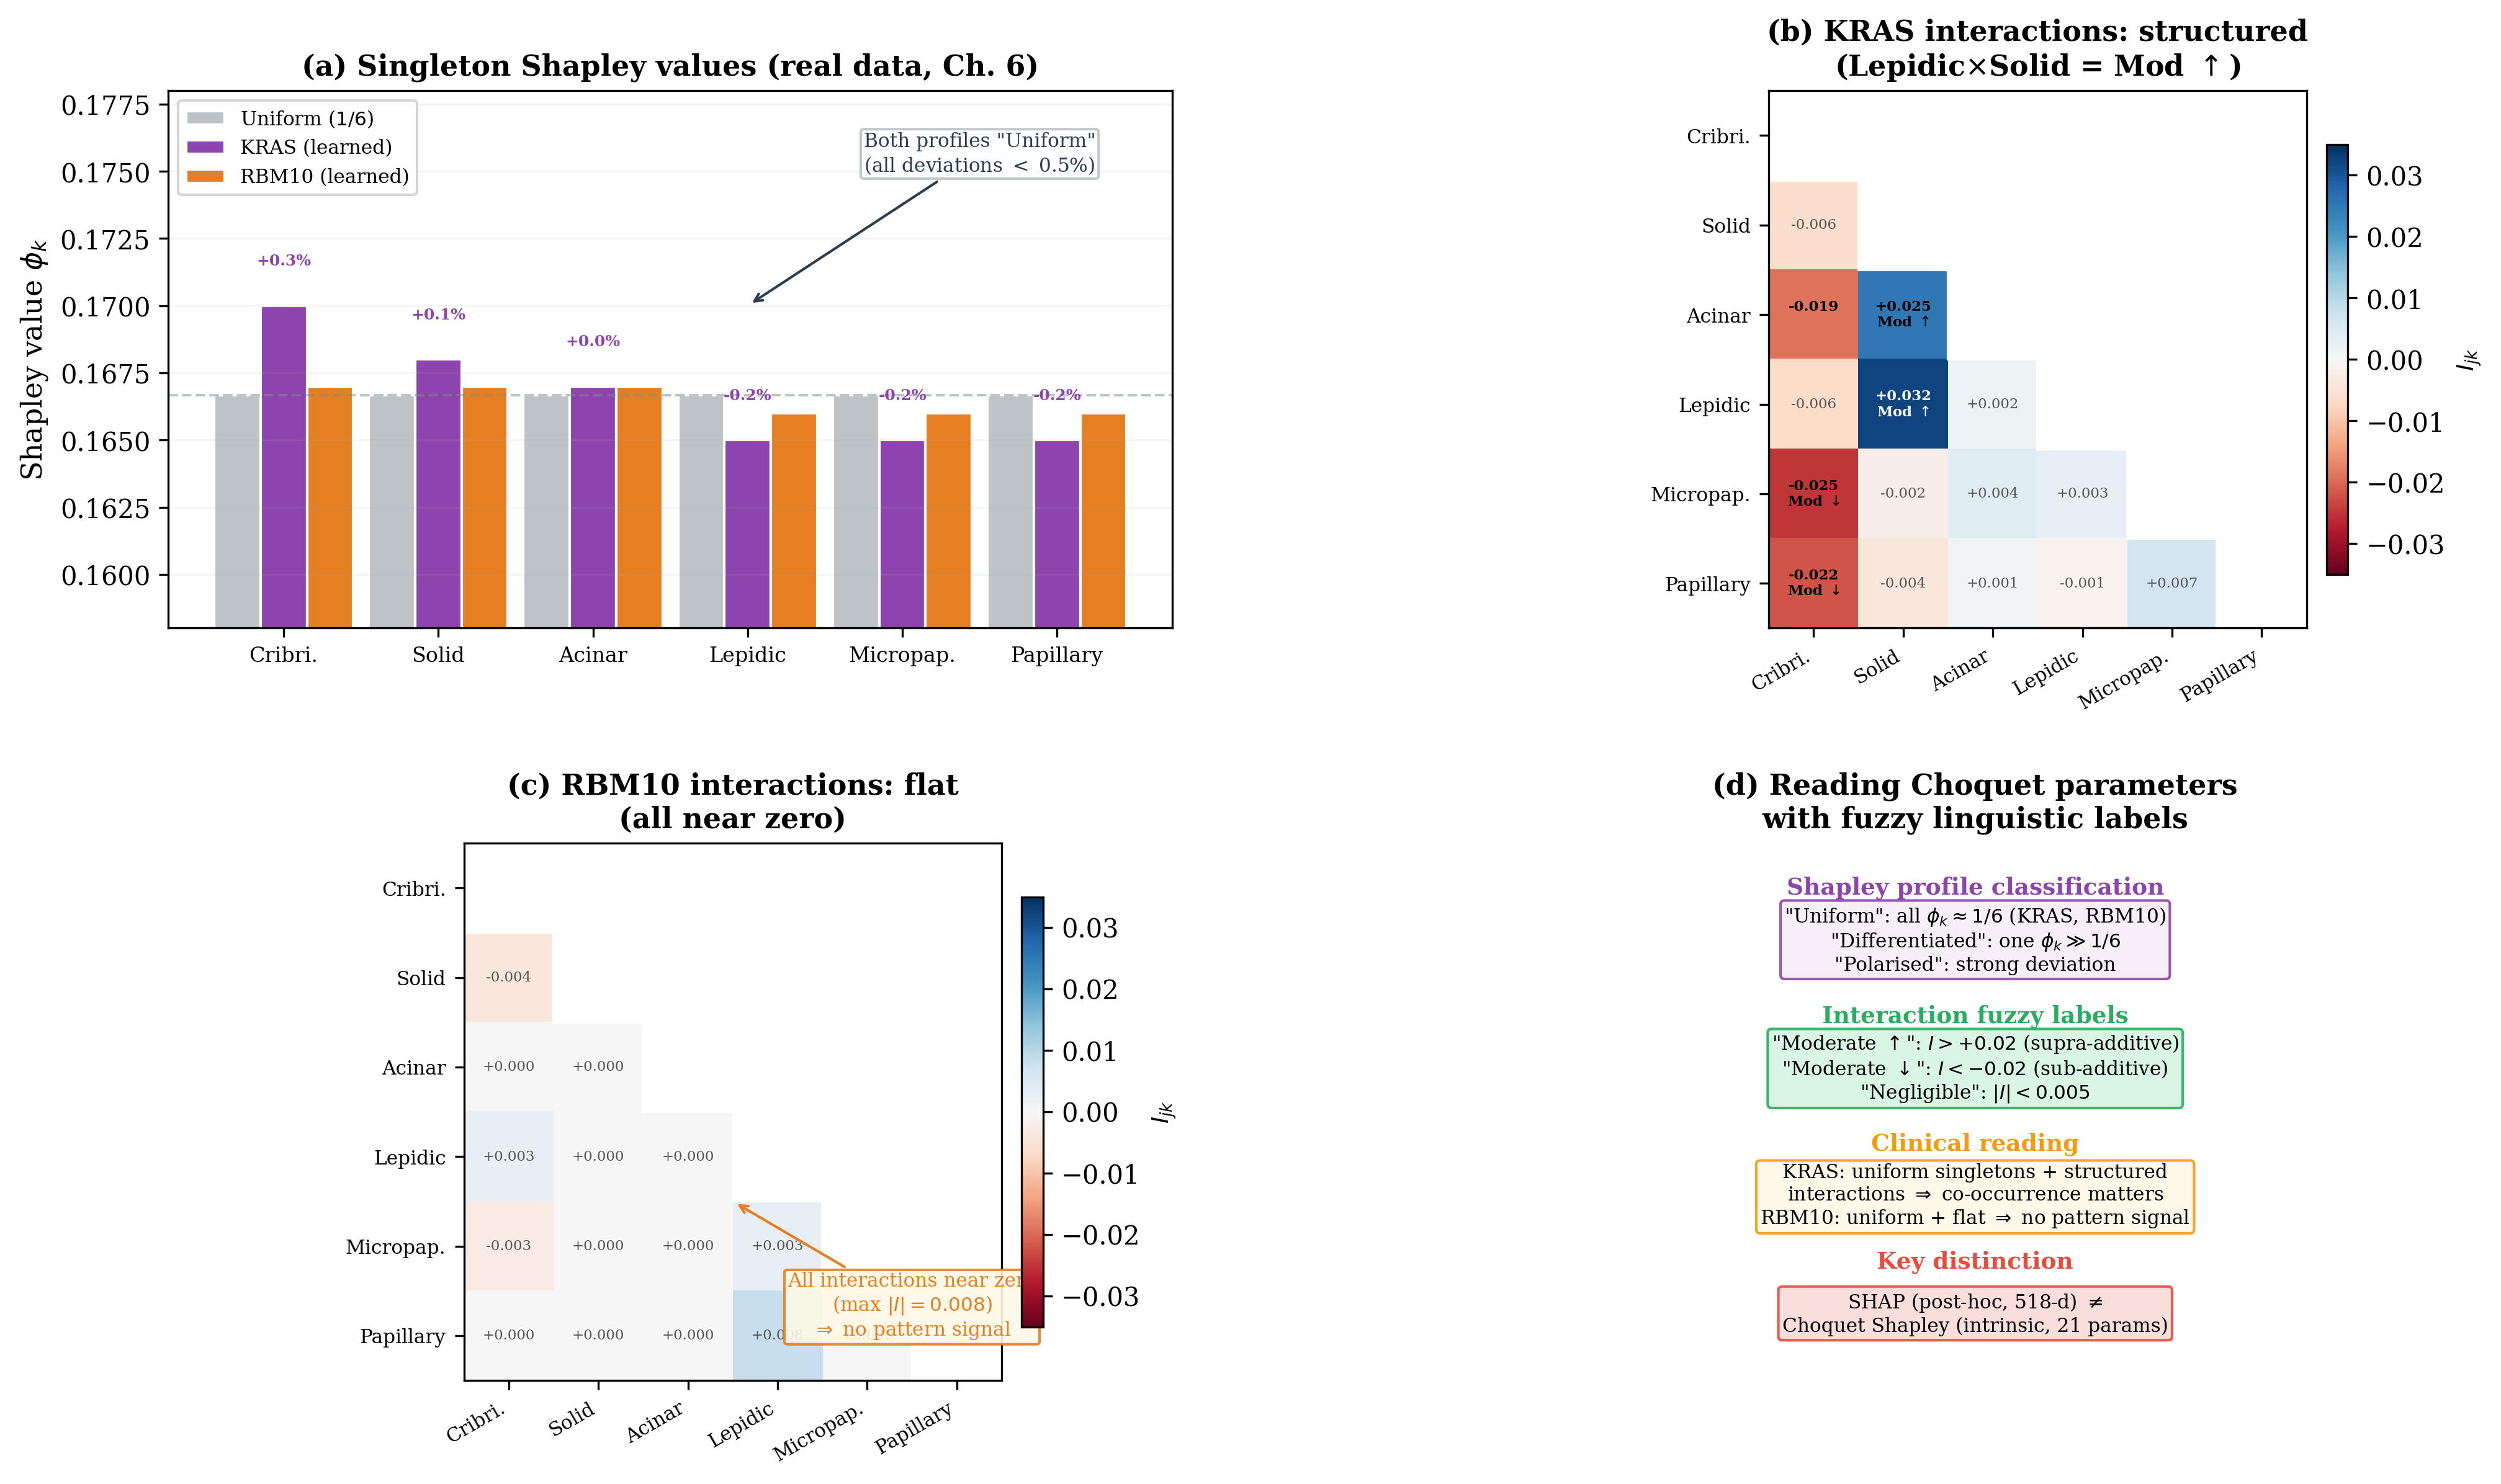
\includegraphics[width=\textwidth]{chapters/figures/choquet_interpretability.png}
\caption[Intrinsic interpretability of the Choquet fuzzy measure
(KRAS vs RBM10, real data)]{%
    Intrinsic interpretability of the learned Choquet fuzzy measure
    using \textbf{real values} from trained FC-MIL checkpoints
    (Chapter~\ref{ch:evaluation}).
    \textbf{(a)}~Singleton Shapley values for KRAS (purple) and
    RBM10 (orange): both profiles are near-uniform
    ($\phi_k \approx 1/6$, deviations $< 0.5\%$), meaning no
    single pattern dominates for either gene.
    \textbf{(b)}~KRAS interaction heatmap: structured interactions
    emerge despite uniform singletons.
    Lepidic$\times$solid ($I = +0.032$, ``Moderate~$\uparrow$'')
    indicates supra-additive co-occurrence; micropapillary$\times$%
    cribriform ($I = -0.025$, ``Moderate~$\downarrow$'') indicates
    overlapping information.
    Fuzzy labels are computed by trapezoidal membership functions
    (Section~\ref{sec:meth:interp:fuzzy_labels}).
    \textbf{(c)}~RBM10 interaction heatmap: all indices near zero
    (max $|I| = 0.008$), confirming no pattern signal---an order
    of magnitude weaker than KRAS.
    \textbf{(d)}~Guide for reading Choquet parameters with fuzzy
    linguistic labels, and the key distinction between post-hoc
    SHAP (518-d) and intrinsic Choquet Shapley values (21 params).}
\label{fig:choquet_interpretability}
\end{figure}


% ============================================================================
\section{Interpretability Framework}
\label{sec:meth:interpretability}
% ============================================================================

The interpretability framework operates at six levels, providing what this thesis terms a \emph{six-level interpretability framework}.

\subsection{Level 1: Spatial Attention Maps}
\label{sec:meth:interp:attention}

For ABMIL-based conditions (B2, B3, PI-ABMIL, A), the attention
weights $\{a_i\}$ from Equation~\ref{eq:gated_attn} are overlaid onto
the WSI as a spatial heatmap.
Tiles with high attention weights are highlighted, indicating regions
the model considers most informative for the mutation prediction.
The concrete rendering choices in LCHAI~v2.0 (which subset of tiles is
displayed, fill colour, contour styling, opacity slider) are
implementation-level decisions reported in
Section~\ref{sec:impl:lchai:ui:viewer}.

\subsection{Level 2: Pattern Attribution}
\label{sec:meth:interp:patterns}

For conditions that incorporate pattern information (B3, PI-ABMIL, A, FC-MIL), each tile's predicted pattern class $\hat{y}_i$ is overlaid onto the WSI as a categorical colour map.
This allows the pathologist to assess whether the attended regions (Level~1) correspond to clinically expected patterns (e.g., TP53-attended tiles should be predominantly solid or micropapillary).

When Levels~1 and~2 are combined, the resulting visualisation shows
both \emph{where} the model attends and \emph{what} the model sees
at those locations, providing a clinically verifiable chain of
reasoning.
For example, on slide TCGA-99-8025
(Section~\ref{sec:eval:interp:attention}):
\begin{quote}
``The model predicts TP53 mutation with $P(\text{mut}) = 0.951$
(Conclusive) because it attends to texture-variant subregions within
a slide dominated by micropapillary morphology (91.5\%), with minor
solid (0.56\%) and cribriform (1.6\%) components---high-grade patterns
associated with TP53-driven genomic
instability~\cite{ahn2022tp53highgrade}.''
\end{quote}

\subsection{Level 3: Feature Attribution via SHAP}
\label{sec:meth:interp:shap}

For the floor baseline B1 (XGBoost),
TreeSHAP~\cite{lundberg2020treeshap} provides exact Shapley values
for each of the seven slide-level features.
For ABMIL conditions, DeepSHAP~\cite{lundberg2017shap} attributes the
prediction to individual dimensions of the tile representation
$\mathbf{h}_i$.
In PI-ABMIL, the SHAP decomposition distinguishes contributions from
the CTransPath embedding dimensions (positions 0--511) versus the
pattern probability dimensions (positions 512--517), quantifying
the relative importance of visual features versus pattern knowledge
for each gene (see Equation~\ref{eq:shap_split} in
Section~\ref{sec:bg:shap} for the per-group mean computation).
The resulting embedding/pattern balance is further classified by the
fuzzy linguistic label system (Level~6,
Section~\ref{sec:meth:interp:fuzzy_labels}) into calibrated terms
such as ``Embedding-Led'' or ``Pattern-Dominated,'' which are
displayed in the LCHAI~v2.0 Analysis tab and injected into
LLM-generated explanations.

\subsection{Level 4: Choquet Shapley Values (Artefact 3 Only)}
\label{sec:meth:interp:choquet_shapley}

For the FC-MIL condition (FC), the learned Shapley values and
interaction indices provide a fourth level of interpretability that is
\emph{intrinsic} to the model rather than post-hoc.
FC-MIL achieves the highest cohort-mean AUROC for KRAS and RBM10
on the K-fold benchmark (Finding~2 in Chapter~\ref{ch:evaluation}),
but the two cases are asymmetric: on KRAS the Choquet branch
captures a genuine inter-pattern interaction
(lepidic$\times$solid synergy that proxies the missing invasive
mucinous class), whereas on RBM10 the branch is empty---a uniform
fuzzy measure with all interaction indices below $\pm 0.01$---and
the lift originates in the shared embedding pathway, so RBM10
serves as an architectural negative control rather than as evidence
of inter-pattern signal (Chapter~\ref{ch:evaluation},
Section~\ref{sec:eval:interp:choquet}).
The intrinsic Shapley values and interaction indices are therefore
clinically actionable primarily for KRAS, while for RBM10 they
formalise the \emph{absence} of pattern-level signal; for the
remaining four genes FC-MIL runs as a complementary analysis
alongside the primary B2 or PI-ABMIL prediction.
Table~\ref{tab:expected_associations} lists the population-level
pattern--mutation associations from the clinical literature against
which the learned Choquet parameters can be validated.

\begin{table}[ht!]
\centering
\small
\caption[Expected pattern--mutation associations from clinical
literature.]{Expected pattern--mutation associations from clinical
literature, used to validate learned Choquet parameters.
FC-MIL is the primary method for KRAS and RBM10 (bold);
for the remaining genes it provides complementary analysis.
The ``Expected'' column reflects population-level associations;
the actual learned Shapley values
(Chapter~\ref{ch:evaluation}, Table~\ref{tab:choquet_shapley}) may
differ due to data scarcity and the absence of certain morphological
classes (e.g., IMA for KRAS) in the 6-class ANORAK taxonomy.}
\label{tab:expected_associations}
\begin{tabular}{p{1.4cm} p{4.2cm} p{5.5cm} p{2.5cm}}
\hline
\textbf{Gene} & \textbf{Expected pattern signal} &
\textbf{Evidence} & \textbf{FC-MIL role} \\
\hline
\textit{TP53}  & Solid, micropapillary &
  Nuclear pleomorphism, high grade~\cite{ahn2022tp53highgrade} &
  Complementary \\
\textbf{\textit{KRAS}}  & Solid; IMA (not in ANORAK) &
  IMA enriched for G12D~\cite{shim2015krasmucinous};
  without IMA class, expect near-uniform singletons with
  structured interactions &
  \textbf{Primary} \\
\textit{EGFR}  & Lepidic, papillary &
  Low atypia, indolent growth~\cite{yoshizawa2013egfrmorph} &
  Complementary \\
\textit{STK11} & High entropy (no dominant pattern) &
  Reduced TILs; ``cold'' micro-environment~\cite{skoulidis2015krassubsets,skoulidis2018stk11pd1} &
  Complementary \\
\textit{KEAP1} & Less pattern-specific~\cite{li2011keap1papillary} &
  Oxidative stress pathway~\cite{tcga2014luad} &
  Complementary \\
\textbf{\textit{RBM10}} & No established correlate &
  RNA splicing regulator; no known morphological
  signature~\cite{tcga2014luad}; expect flat measure &
  \textbf{Primary} \\
\hline
\end{tabular}
\end{table}

\subsection{Level 5: Per-Slide Feature Channel Ablation}
\label{sec:meth:interp:ablation}

SHAP (Level~3) reveals how a \emph{single trained model} distributes
its internal attribution across input dimensions.
A distinct and complementary question is whether a feature channel
\emph{actually helps or harms} prediction on a given slide.
To answer this, LCHAI~v2.0 performs a \textbf{per-slide feature
channel ablation} (cf.\ Section~\ref{sec:bg:channel_ablation}) by
running three \emph{separately trained} models on the same tile set:

\begin{enumerate}
    \item \textbf{Combined} ($f_{\text{PI}}$): the PI-ABMIL model,
    operating on the full 518-d representation
    $\mathbf{h}_i = [\mathbf{x}_i \,\|\, \mathbf{p}_i]$.
    \item \textbf{Embeddings-only} ($f_{\text{B2}}$): the ABMIL model
    trained on CTransPath embeddings alone (condition~B2),
    $\mathbf{h}_i = \mathbf{x}_i \in \mathbb{R}^{512}$.
    \item \textbf{Patterns-only} ($f_{\text{B3}}$): the ABMIL model
    trained on fuzzy pattern probabilities alone (condition~B3),
    $\mathbf{h}_i = \mathbf{p}_i \in \Delta^5$.
\end{enumerate}

For a slide with tile embeddings $\{\mathbf{x}_i\}$ and pattern
probabilities $\{\mathbf{p}_i\}$, the three models produce three
mutation probabilities:
\begin{equation}
\label{eq:ablation_perslide}
P_{\text{comb}} = \sigma(f_{\text{PI}}(\{\mathbf{h}_i\})), \quad
P_{\text{emb}} = \sigma(f_{\text{B2}}(\{\mathbf{x}_i\})), \quad
P_{\text{pat}} = \sigma(f_{\text{B3}}(\{\mathbf{p}_i\})),
\end{equation}
where $\sigma$ is the sigmoid function.
The \textbf{pattern ablation delta} is then:
\begin{equation}
\label{eq:delta_pattern}
\Delta_{\text{pat}} = P_{\text{comb}} - P_{\text{emb}}.
\end{equation}

Figure~\ref{fig:ablation_causal_chain} illustrates the complete causal
chain from tile features to $P(\text{mut})$ for the three ablation
models.

\begin{figure}[ht!]
\centering
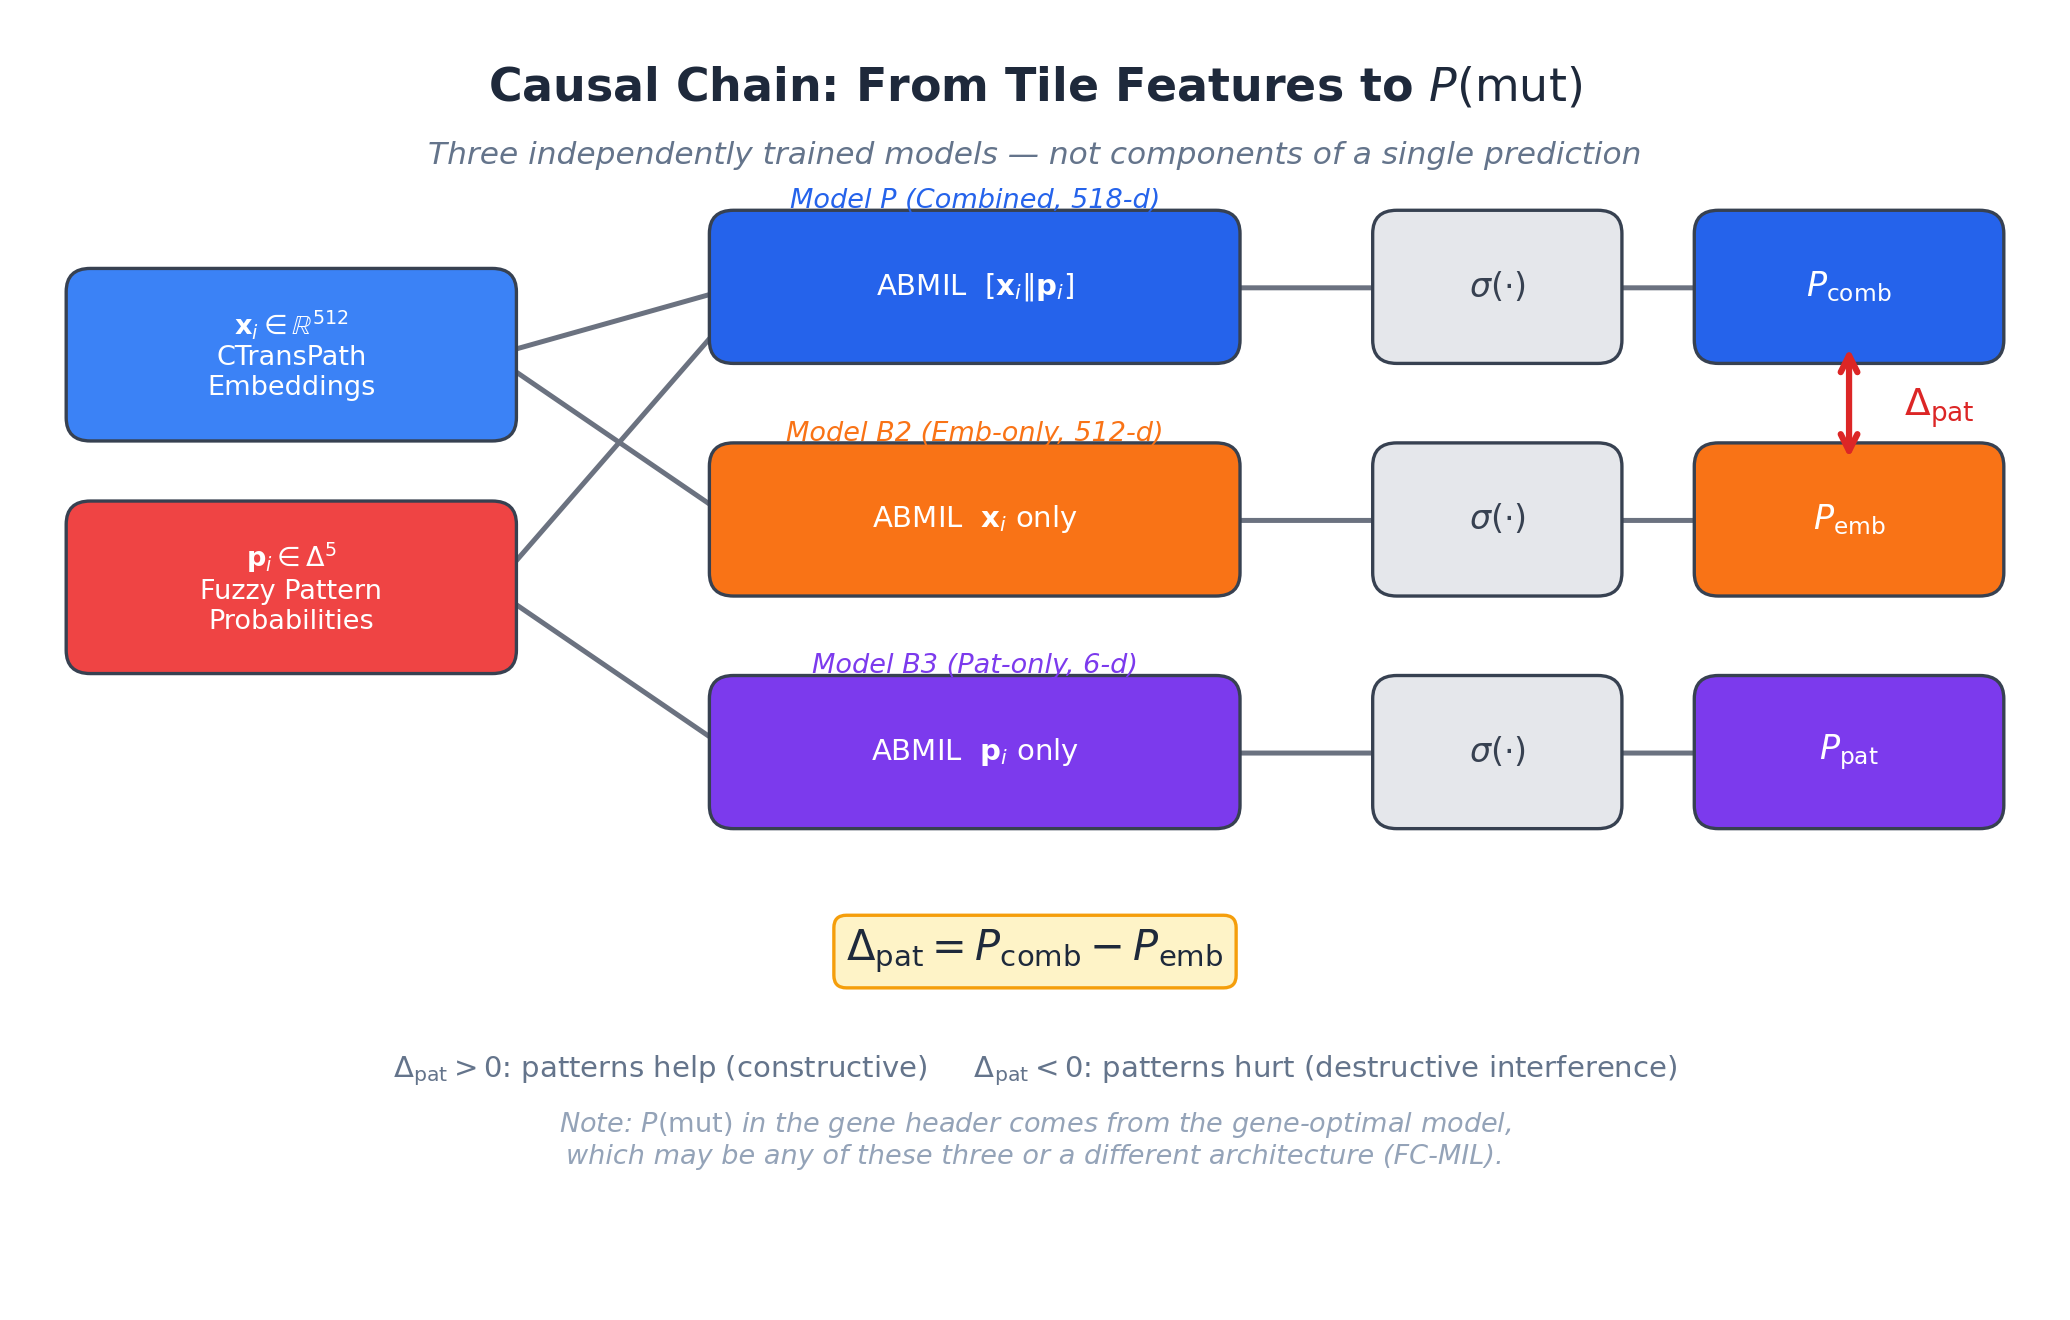
\includegraphics[width=\textwidth]{chapters/figures/ablation_causal_chain.png}
\caption[Causal chain from tile features to $P(\text{mut})$ in the
ablation framework]{%
    Causal chain from tile features to $P(\text{mut})$.
    Three independently trained ABMIL models operate on different input
    representations: Combined (518-d), Embeddings-only (512-d), and
    Patterns-only (6-d).
    Each model produces its own $P(\text{mut})$ via a sigmoid
    classification head.
    The pattern ablation delta $\Delta_{\text{pat}} = P_{\text{comb}} -
    P_{\text{emb}}$ measures whether adding pattern features helps or
    harms the prediction.
    The $P(\text{mut})$ displayed in the LCHAI~v2.0 interface comes
    from the gene-optimal model (Finding~2), which may differ from any
    of the three ablation models.}
\label{fig:ablation_causal_chain}
\end{figure}

When $\Delta_{\text{pat}} > 0$, adding pattern features to
embeddings improves the prediction on this specific slide; when
$\Delta_{\text{pat}} < 0$, pattern features introduce
\emph{interference} that degrades it.

\textbf{Why separately trained models.}
Unlike gradient-based methods (SHAP) that explain a single model's
internals, channel ablation requires models that were \emph{trained}
with the ablated input space---otherwise the model would simply see
zeros or noise in the missing dimensions, which does not reflect its
true capability without those features.
The five-fold cross-validated B2 and B3 checkpoints from the
evaluation protocol (Section~\ref{sec:meth:eval:cv}) serve this
purpose: they represent the best each channel can achieve in
isolation, trained and selected under identical conditions.

\textbf{Interpretation alongside SHAP.}
Combining SHAP (Level~3) with ablation (Level~5) yields a richer
picture:
\begin{itemize}
    \item \textbf{High SHAP pattern attribution + positive
    $\Delta_{\text{pat}}$}: The model attends to patterns AND they
    help. Example: KRAS (SHAP 41\% pattern, $\Delta = +7.6$\,pp).
    \item \textbf{High SHAP pattern attribution + negative
    $\Delta_{\text{pat}}$}: The model attends to patterns but they
    \emph{hurt}. Example: KEAP1 (SHAP 60\% pattern,
    $\Delta = -44.7$\,pp).
    \item \textbf{Low SHAP pattern attribution + negative
    $\Delta_{\text{pat}}$}: The model largely ignores patterns, yet
    even the residual attention degrades prediction. Example: STK11
    (SHAP 10\% pattern, $\Delta = -5.5$\,pp).
\end{itemize}
Figure~\ref{fig:shap_ablation_quadrant} maps all six genes into this
two-dimensional space, revealing the dissociation between
\emph{attribution} (what the model attends to) and \emph{utility}
(what actually helps)---a key finding of the evaluation
(Chapter~\ref{ch:evaluation}).

\begin{figure}[ht!]
\centering
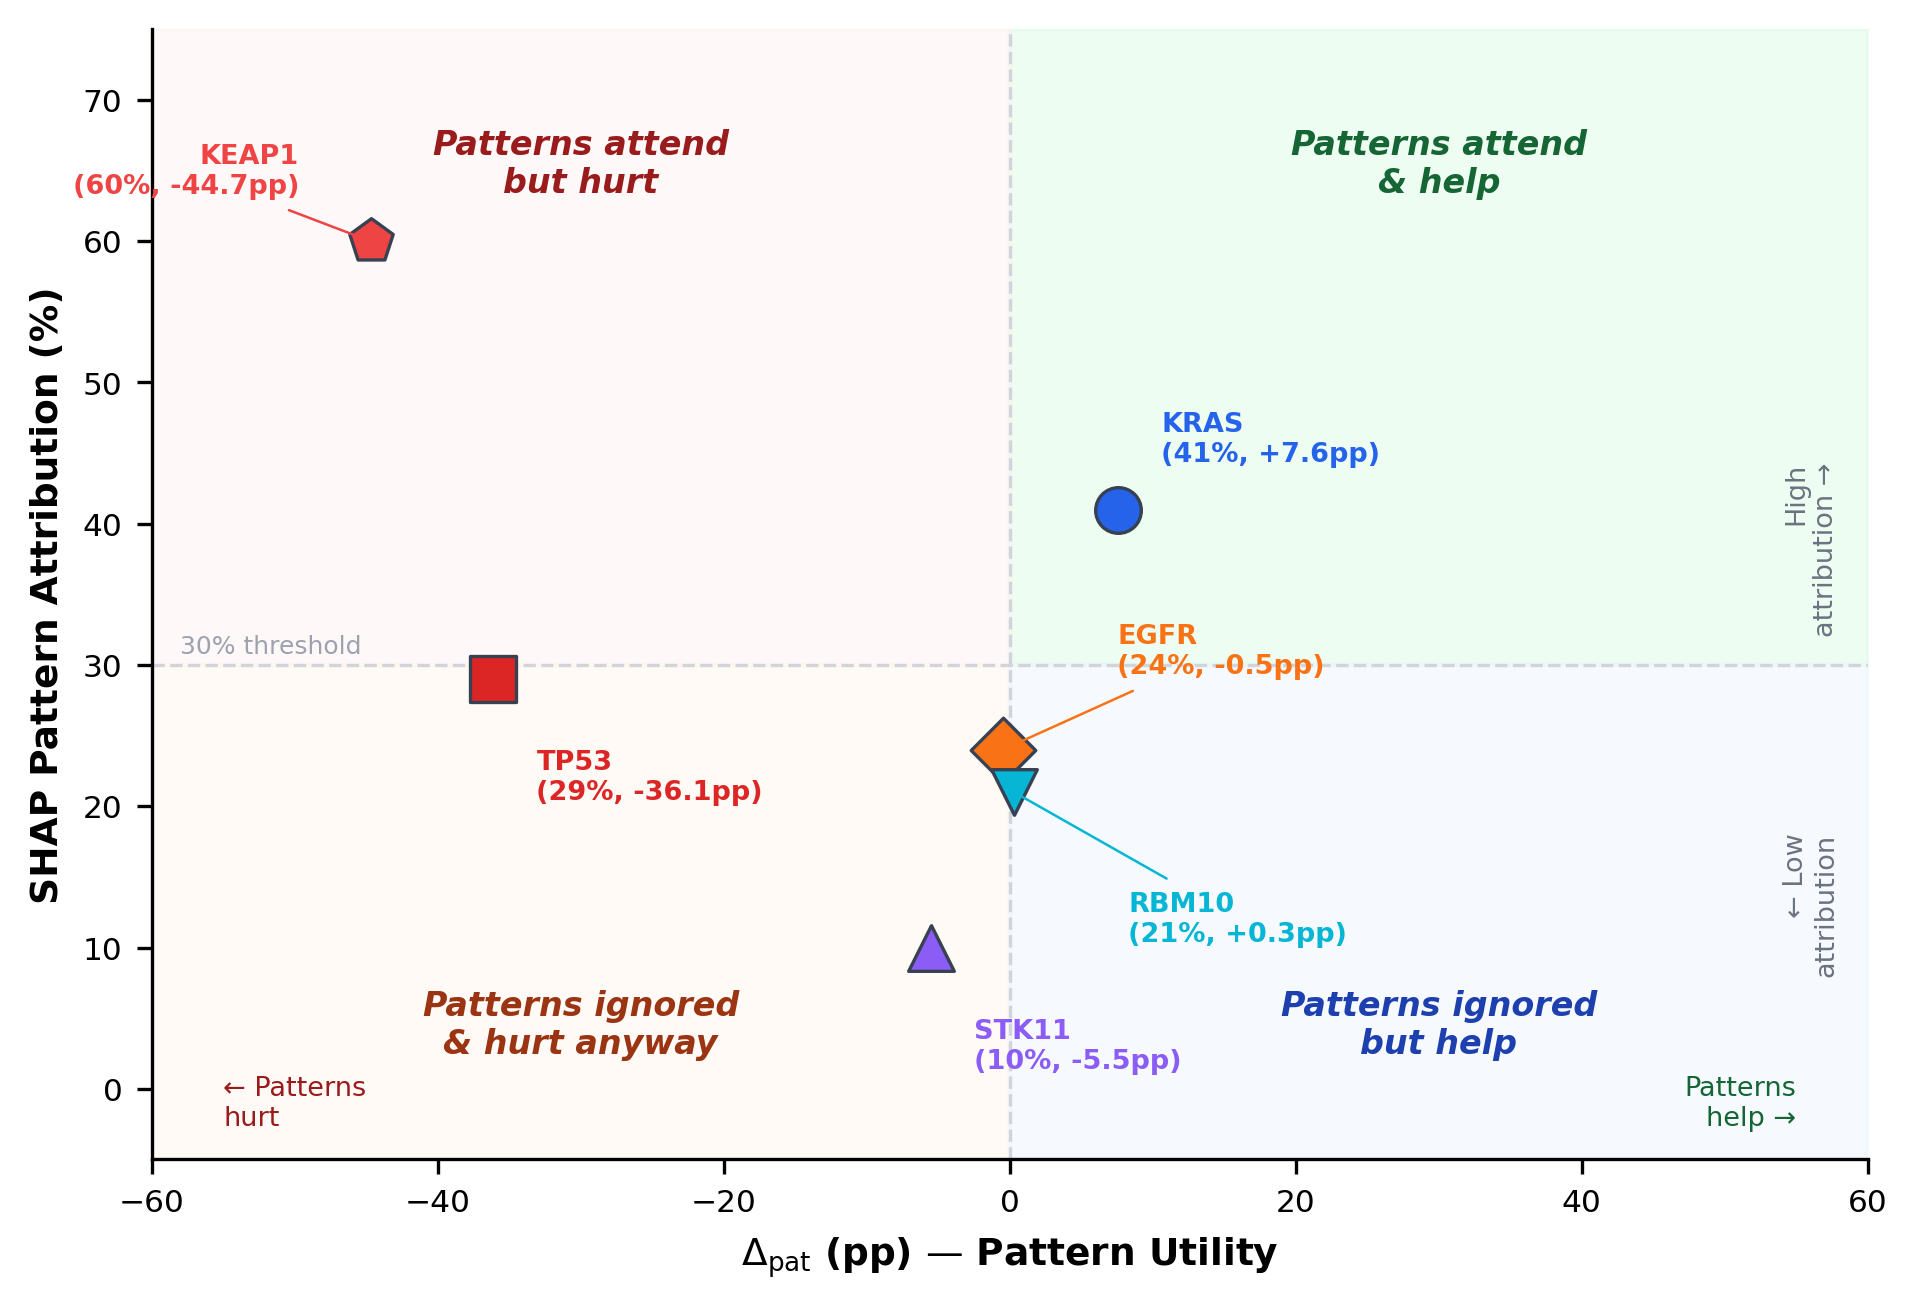
\includegraphics[width=0.85\textwidth]{chapters/figures/shap_ablation_quadrant.png}
\caption[Attribution vs utility: SHAP pattern attribution versus
ablation delta for six genes]{%
    Attribution versus utility for the six target genes on
    representative TCGA-LUAD slides.
    The $x$-axis shows $\Delta_{\text{pat}}$ (pattern ablation delta
    in percentage points); the $y$-axis shows SHAP pattern attribution
    (\%).
    KRAS occupies the top-right quadrant (patterns attend and help);
    KEAP1 occupies the top-left (patterns attend but hurt---the most
    clinically dangerous miscalibration);
    STK11 falls in the bottom-left (patterns ignored and still degrade
    prediction).
    This dissociation motivates the gene-dependent method selection
    strategy (Finding~2).}
\label{fig:shap_ablation_quadrant}
\end{figure}

\subsection{Per-Slide vs.\ Per-Gene Model Arbitration: Why Model
Selection Happens at the Cohort Level}
\label{sec:meth:interp:gene_vs_slide_selection}

The Level~5 ablation panel
(Section~\ref{sec:meth:interp:ablation}) surfaces, for each slide,
the prediction $P_{\text{comb}}$ of the gene-optimal model and the
counterfactual prediction $P_{\text{emb}}$ of the embeddings-only
ablation model.
On a non-trivial fraction of slides the two values fall on
opposite sides of the $0.5$ decision threshold---one would yield
a true positive, the other a false negative.
This directly raises the question:

\begin{quote}
    \emph{If the ablation reveals that another model would have
    predicted better on this specific slide, why does LCHAI~v2.0
    not switch to that model in deployment?}
\end{quote}

LCHAI~v2.0 deliberately fixes the model choice \emph{at the gene
level}, before any test slide is examined (Finding~2,
Section~\ref{sec:eval:mutation:finding2}).
Per-slide arbitration is rejected for four reasons that follow
from the statistical structure of the problem rather than from
engineering preference.

\textbf{(R1) Circularity: per-slide selection requires the
label.}
The statement \emph{``the embeddings-only model would have
predicted better on this slide''} is only verifiable in
retrospect, against the ground-truth mutation status established
by DNA sequencing.
In a deployment setting the system has no access to that label;
it is precisely what the predictor is trying to estimate.
Any selection rule of the form \emph{``use the model whose output
matches the truth on this slide''} is therefore not implementable
as a runtime policy---it can only be applied post-hoc when the
result is already known, which is cherry-picking, not prediction.

\textbf{(R2) Score incomparability across separately trained
models.}
The three ablation models---Combined ($f_{\text{PI}}$),
Embeddings-only ($f_{\text{B2}}$), Patterns-only
($f_{\text{B3}}$)---are independently trained networks with
different input spaces, different decision surfaces, and different
implicit calibration of their sigmoid output heads.
A value of $P = 0.69$ produced by $f_{\text{B2}}$ and a value of
$P = 0.25$ produced by $f_{\text{PI}}$ do not lie on a common
probability scale; their thresholds at $0.5$ correspond to
different decision regions in feature space.
Comparing them slide-by-slide and selecting the larger value
amounts to taking the maximum of two scores from differently
calibrated classifiers, which is not a calibrated probability
estimate of any well-defined event.

\textbf{(R3) The $\max$ rule is not generally a better
classifier.}
Even setting calibration aside, the AUROC of the rule
$s_{\max}(\mathbf{x}) = \max(s_A(\mathbf{x}), s_B(\mathbf{x}))$
is not, in general, an upper bound on
$\max(\mathrm{AUROC}(s_A), \mathrm{AUROC}(s_B))$.
Taking the maximum inflates scores in the mutant cohort
(potentially recovering some false negatives) but \emph{also}
inflates scores in the wild-type cohort (creating new false
positives).
For low-prevalence genes such as KEAP1 ($14.3\%$ mutation rate),
the precision penalty of these new false positives typically
matches or exceeds the recall benefit of the rescued false
negatives, so the net effect on cross-validated AUROC is empirical
and frequently negative; in particular, ensemble literature
consistently shows that na\"{\i}ve $\max$-of-experts is dominated
by both single-expert selection and weighted averaging.

\textbf{(R4) Per-slide variance is inherent and is what AUROC
already quantifies.}
The reported per-gene AUROC values of Chapter~\ref{ch:evaluation}
are 5-fold cross-validated estimates of the expected ranking
quality of each model over the cohort.
PI-ABMIL ranking ahead of B2 on KEAP1 by $+0.013$ AUROC
(Table~\ref{tab:p_vs_b2}, Chapter~\ref{ch:evaluation}) means that
\emph{on average} PI-ABMIL ranks a random KEAP1-mutant slide
higher than a random wild-type slide more often than B2 does.
On any \emph{single} slide either model can lose: the gap between
their per-slide predictions is the same per-slide variance that
the cross-validated mean already integrates over.
Selecting the per-gene best-in-expectation model is therefore the
choice that minimises expected misranking risk under the
constraint that selection must be made before observing the
label.

\begin{figure}[ht!]
\centering
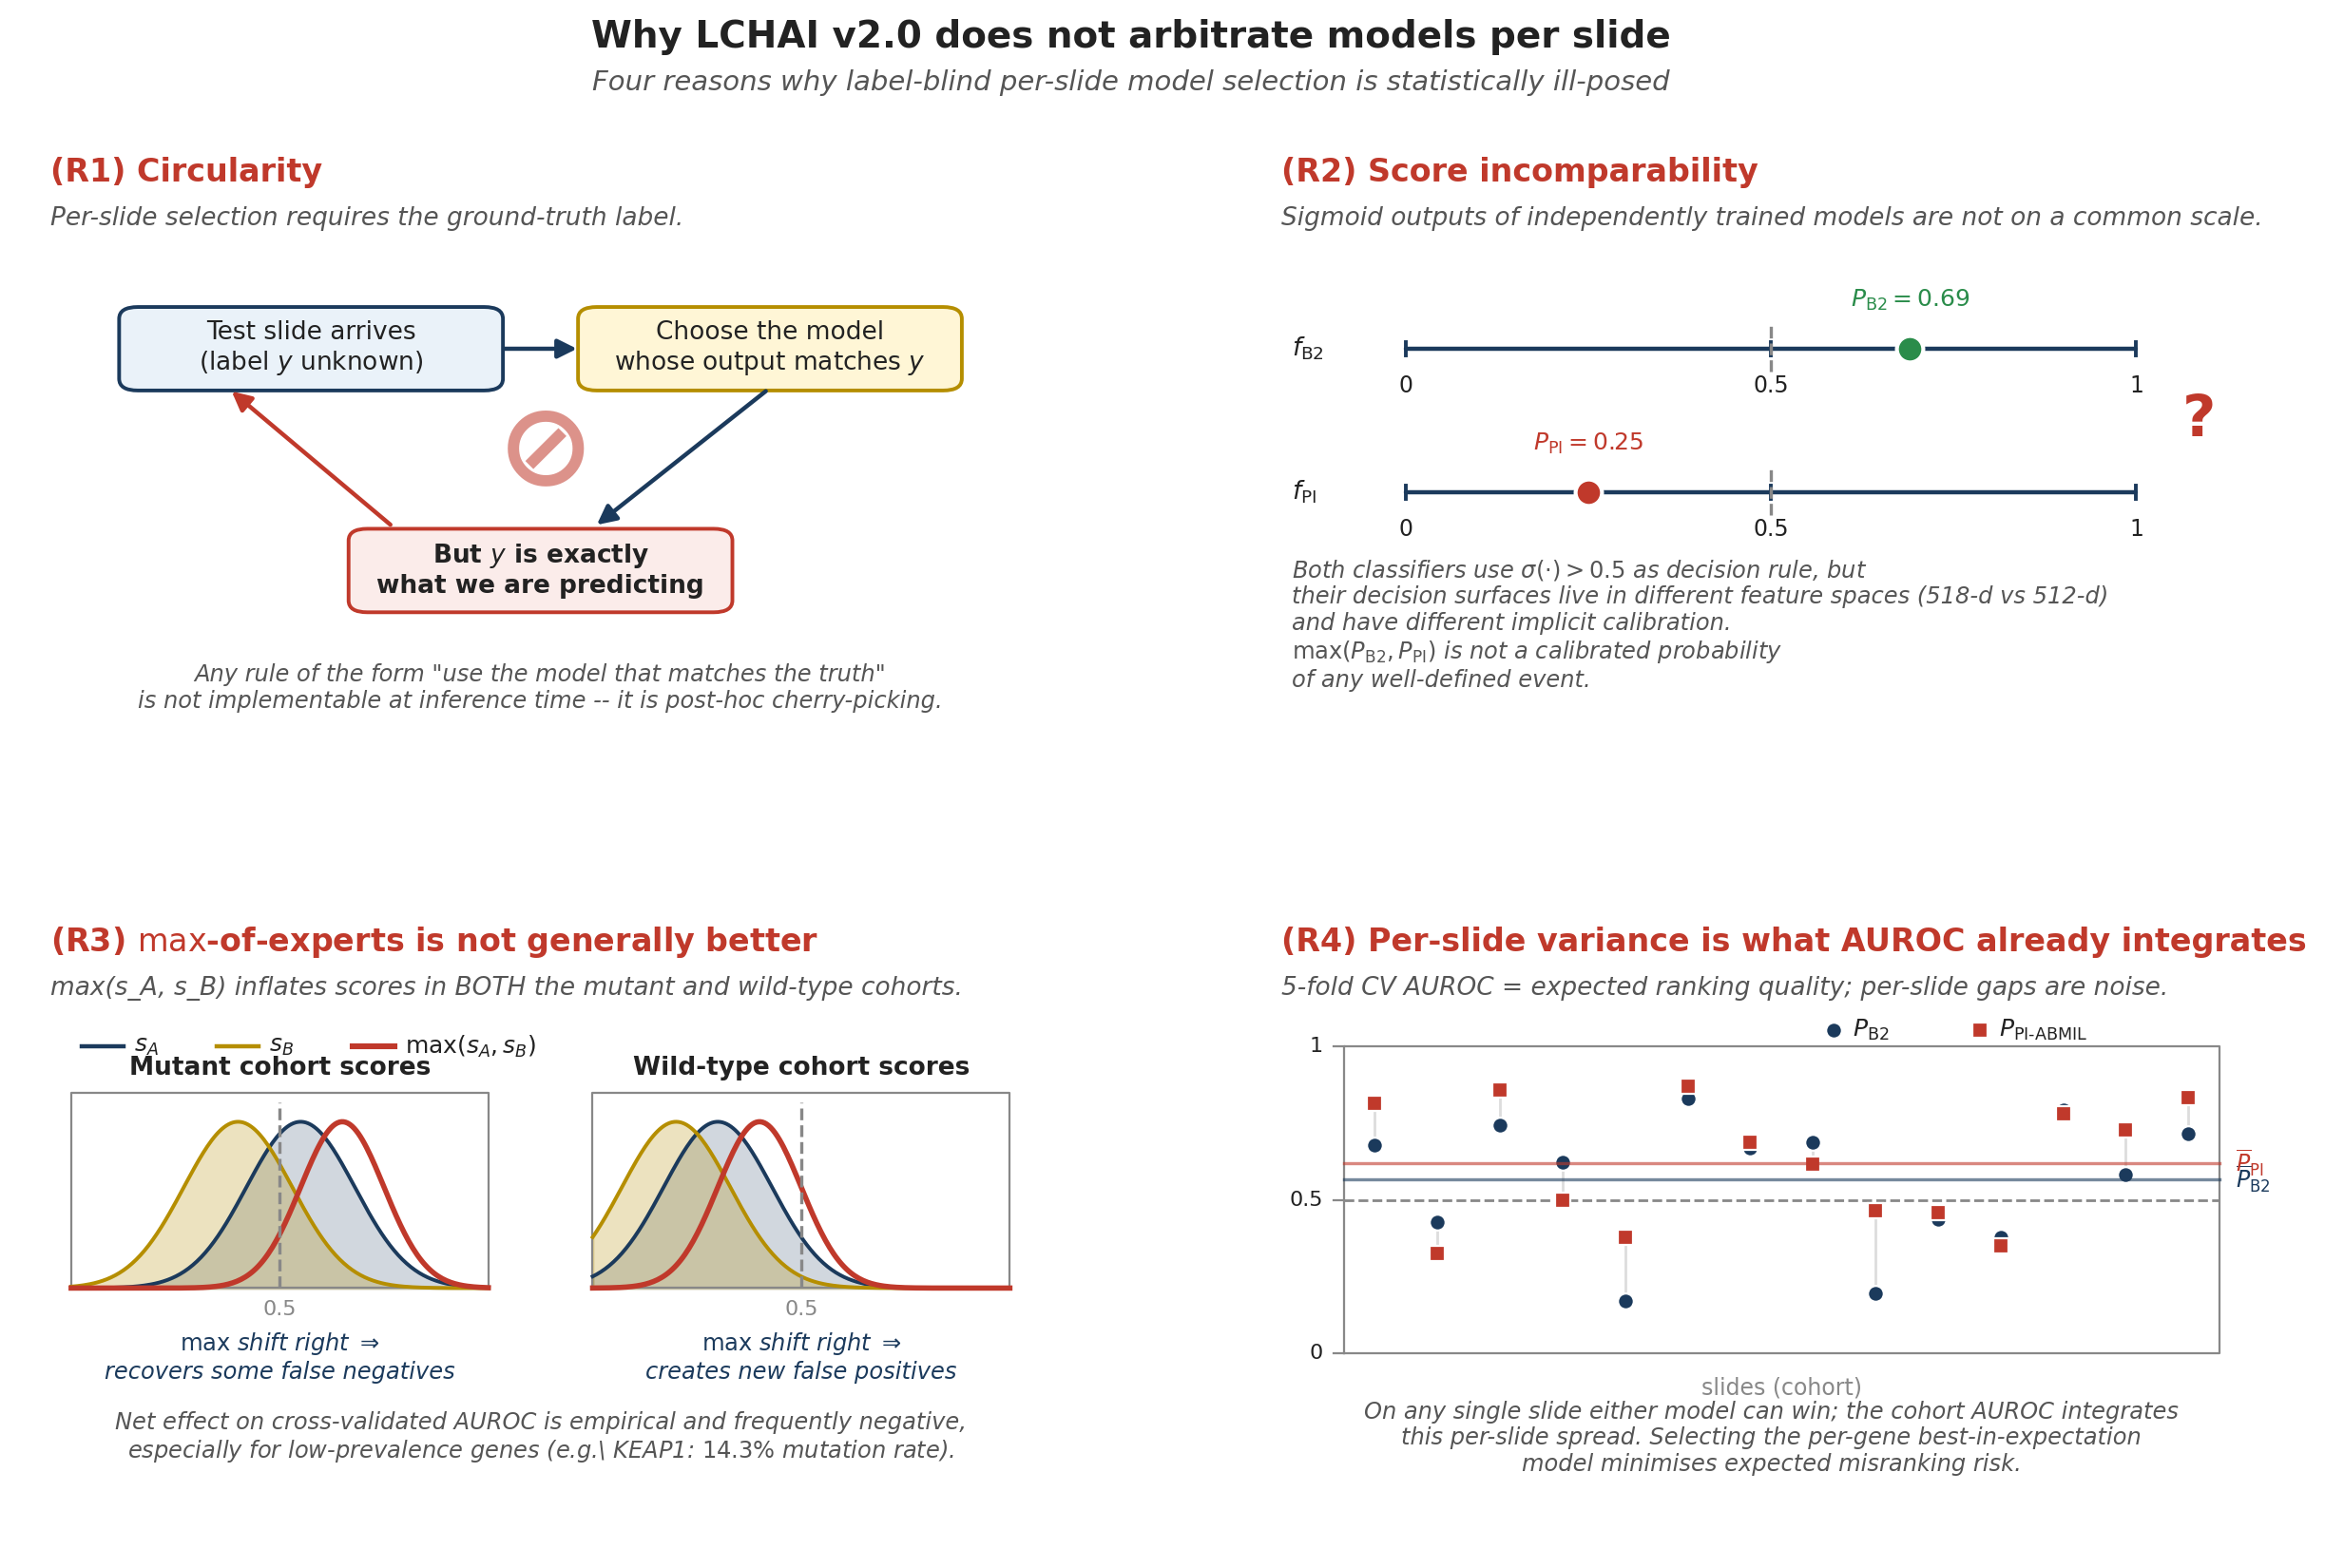
\includegraphics[width=0.97\textwidth]{chapters/figures/per_slide_arbitration_fails.png}
\caption[Why per-slide model arbitration is statistically ill-posed]{%
    Visual summary of the four reasons why LCHAI~v2.0 fixes the
    model choice at the gene level rather than arbitrating models
    per slide.
    \textbf{(R1)~Circularity}---a rule of the form ``use the model
    whose output matches the truth'' requires the very label that
    the predictor is trying to estimate, and so cannot be
    implemented at inference time.
    \textbf{(R2)~Score incomparability}---sigmoid outputs of
    independently trained models live on different scales;
    $\max(P_{\text{B2}}, P_{\text{PI}})$ is not a calibrated
    probability of any well-defined event.
    \textbf{(R3)~$\max$-of-experts is not generally better}---the
    rule shifts scores upwards in \emph{both} the mutant and the
    wild-type cohort, so the gain in recall is generally cancelled
    or exceeded by the loss in precision, especially for
    low-prevalence genes such as KEAP1.
    \textbf{(R4)~Per-slide variance is what AUROC integrates}---on
    any single slide either model can win, but the cross-validated
    AUROC already reports the expected ranking quality across this
    spread; selecting the per-gene best-in-expectation model
    minimises expected misranking risk under label-blind
    deployment.}
\label{fig:per_slide_arbitration_fails}
\end{figure}

Figure~\ref{fig:per_slide_arbitration_fails} summarises the four
arguments in a single diagram and is referenced directly from the
case studies of Chapter~\ref{ch:evaluation} whenever a slide-level
false negative motivates the question of per-slide model
switching (e.g.\ KEAP1 slide
TCGA-49-AAR9, Section~\ref{sec:eval:tcga:keap1}).

\paragraph{The role of the Level~5 ablation panel.}
The ablation panel is therefore an \emph{interpretability}
artefact, not a runtime arbitration mechanism.
On any given slide it surfaces, for the human reader or any
downstream system, three facts: how confident the gene-optimal
model is, how confident the embeddings-only counterfactual would
be, and the magnitude and sign of $\Delta_{\text{pat}}$.
A clinician reading the panel can adjust their confidence in the
displayed $P(\text{mut})$---for example, by treating
slide-specific predictions on heavily negative-$\Delta_{\text{pat}}$
cases with caution---without LCHAI~v2.0 itself
performing a label-blind override that would compromise the
calibration and the cohort-level guarantees described above.

\paragraph{Label-free arbitration as a future-work direction.}
A principled relaxation of the gene-level rule is a
\emph{learnable mixture-of-experts gate} that, from
input features alone, weights the three ablation models
on a per-slide basis.
Such a gate is itself a separate model with its own training,
validation, and overfitting risk, and its evaluation requires
proper held-out cross-validation against the same protocol used
in Chapter~\ref{ch:evaluation}.
This extension is documented in
Section~\ref{sec:disc:future:moe_gate} of
Chapter~\ref{ch:discussion} and is not part of the present
artefact.

\subsection{Level 6: Fuzzy Linguistic Interpretation}
\label{sec:meth:interp:fuzzy_labels}

Levels~1--5 produce numeric outputs whose magnitude is difficult for
clinicians to assess without calibrated reference scales.
Level~6 addresses this by applying trapezoidal fuzzy membership
functions (Section~\ref{sec:bg:fuzzy:sets}) to classify each numeric
output into a \emph{linguistic label}---an intensity term such as
``Moderate~$\uparrow$'' (for a supra-additive interaction index) or
``Embedding-Led'' (for the SHAP balance).
Five fuzzy scales are defined (Table~\ref{tab:fuzzy_scales}):
SHAP Balance, Shapley Profile, Shapley Individual, Interaction Index,
and ABMIL Attention Level.

\begin{table}[ht!]
\centering\small
\caption{Fuzzy linguistic scales for XAI output classification.}
\label{tab:fuzzy_scales}
\begin{tabular}{l l l}
\hline
\textbf{Scale} & \textbf{Input} & \textbf{Labels} \\
\hline
SHAP Balance & Pattern \% & Emb-Dominated, Emb-Led, Balanced, Pat-Led, Pat-Dominated \\
Shapley Profile & spread & Uniform, Near-Uniform, Mod.\ Diff., Strongly Diff., Polarised \\
Shapley Individual & $|\delta_k|$ & Average, Slightly, Moderately, Strongly Above/Below \\
Interaction Index & $|I_{jk}|$ & Negligible, Weak, Moderate, Strong, Very Strong \\
Attention Level & percentile & Very Low, Low, Moderate, High, Very High \\
\hline
\end{tabular}
\end{table}

Figure~\ref{fig:fuzzy_mf_scales} shows the trapezoidal membership
functions for all five scales.
The overlapping regions between adjacent sets reflect the gradual
transition between linguistic categories---a core property of fuzzy
classification that avoids the brittleness of crisp thresholds.

\begin{figure}[ht!]
\centering
\begin{minipage}[t]{0.48\textwidth}
\centering
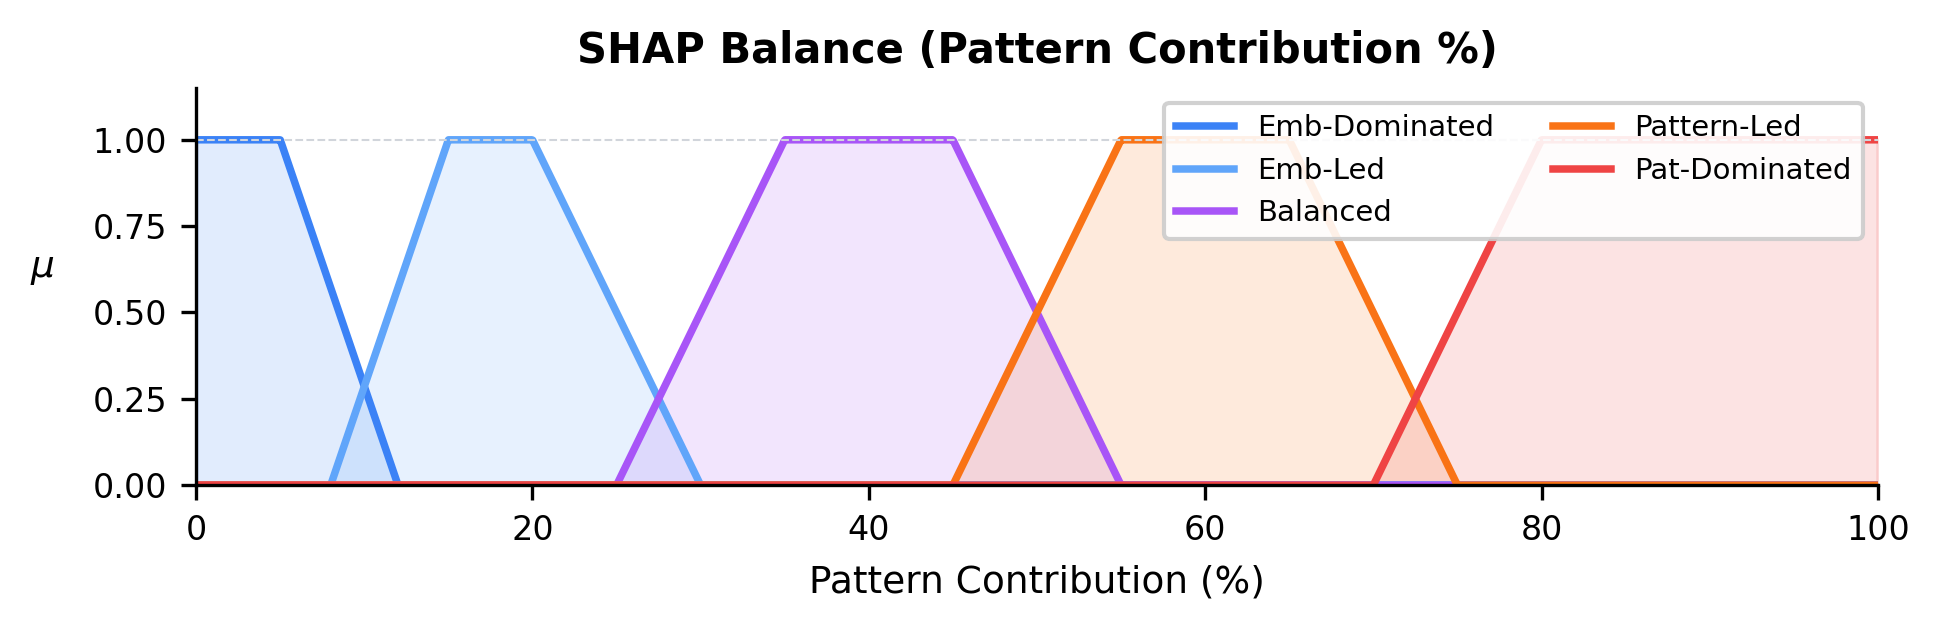
\includegraphics[width=\textwidth]{chapters/figures/fuzzy_mf_shap_balance.png}
\end{minipage}\hfill
\begin{minipage}[t]{0.48\textwidth}
\centering
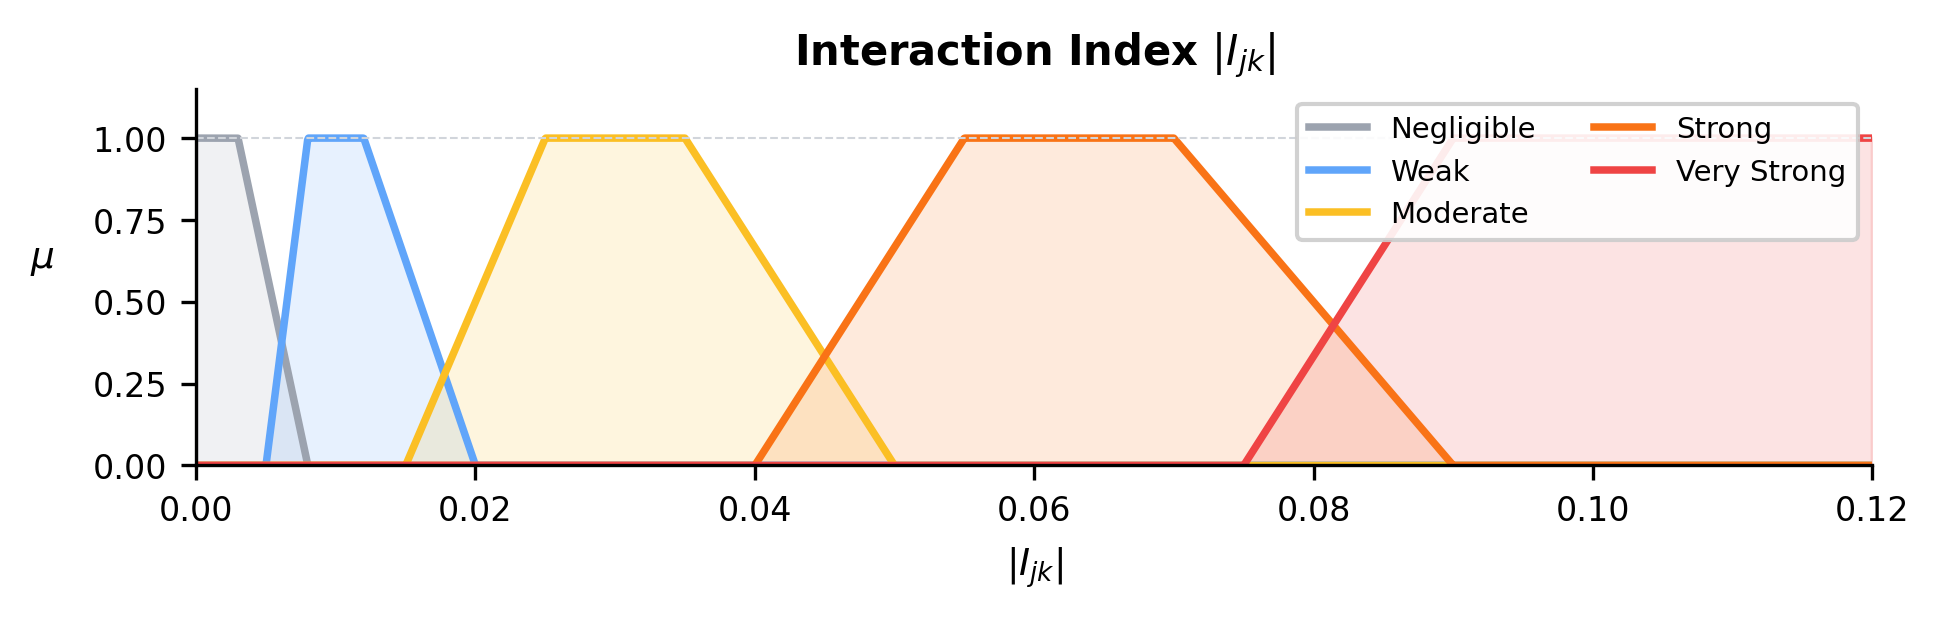
\includegraphics[width=\textwidth]{chapters/figures/fuzzy_mf_interaction_index.png}
\end{minipage}\\[6pt]
\begin{minipage}[t]{0.48\textwidth}
\centering
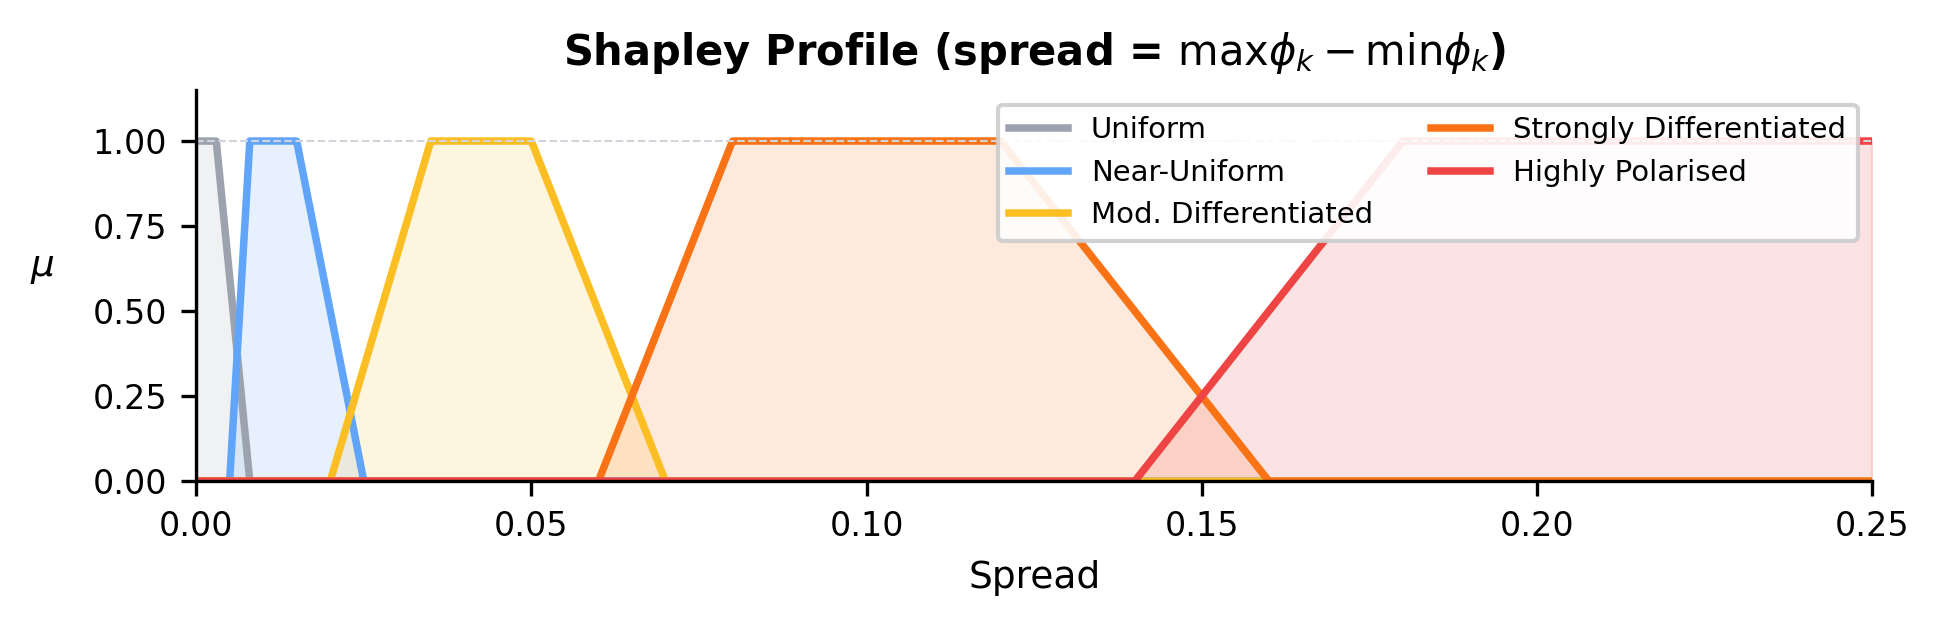
\includegraphics[width=\textwidth]{chapters/figures/fuzzy_mf_shapley_profile.png}
\end{minipage}\hfill
\begin{minipage}[t]{0.48\textwidth}
\centering
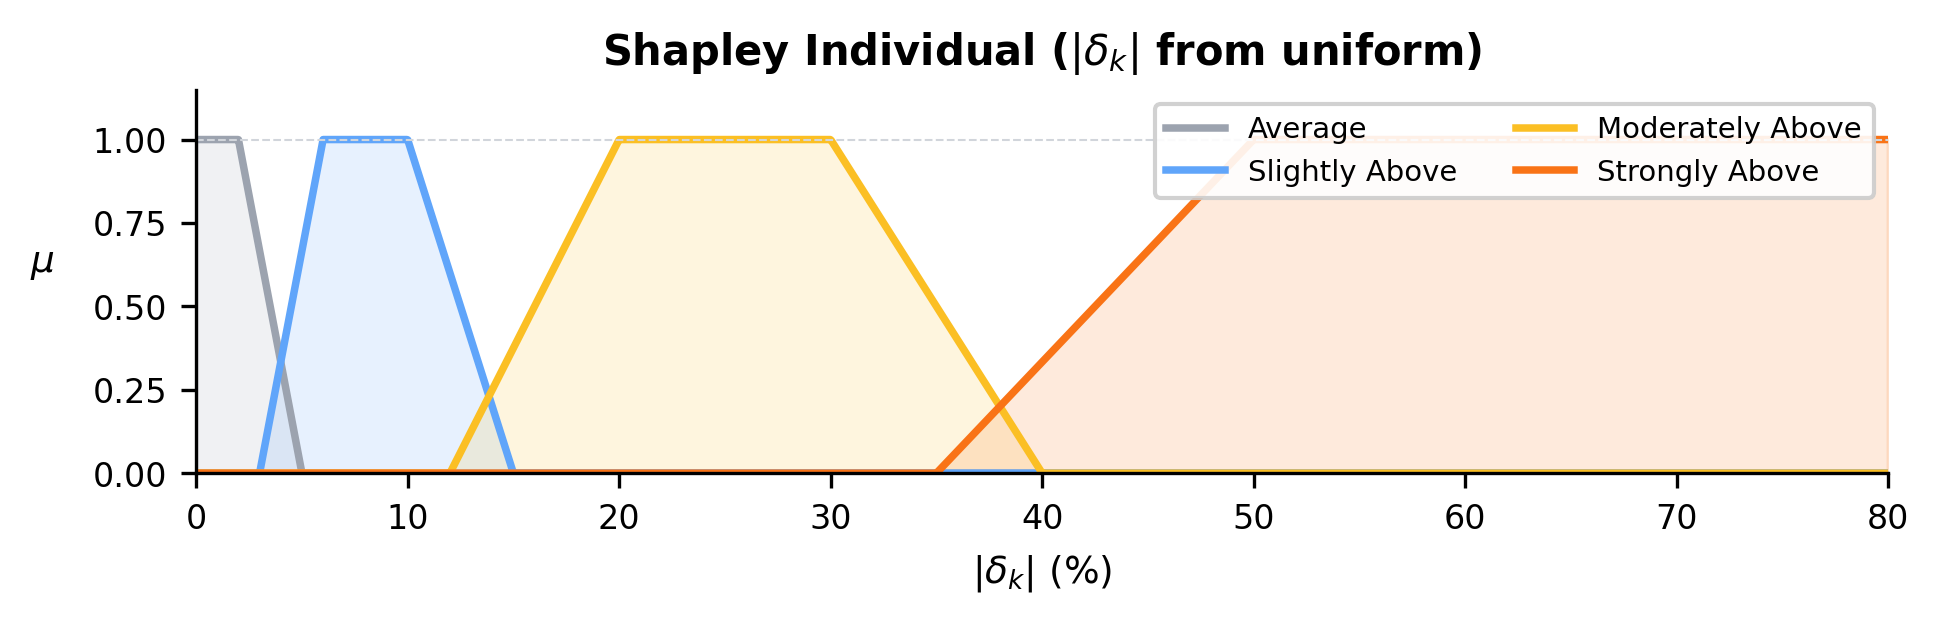
\includegraphics[width=\textwidth]{chapters/figures/fuzzy_mf_shapley_individual.png}
\end{minipage}\\[6pt]
\begin{minipage}[t]{0.48\textwidth}
\centering
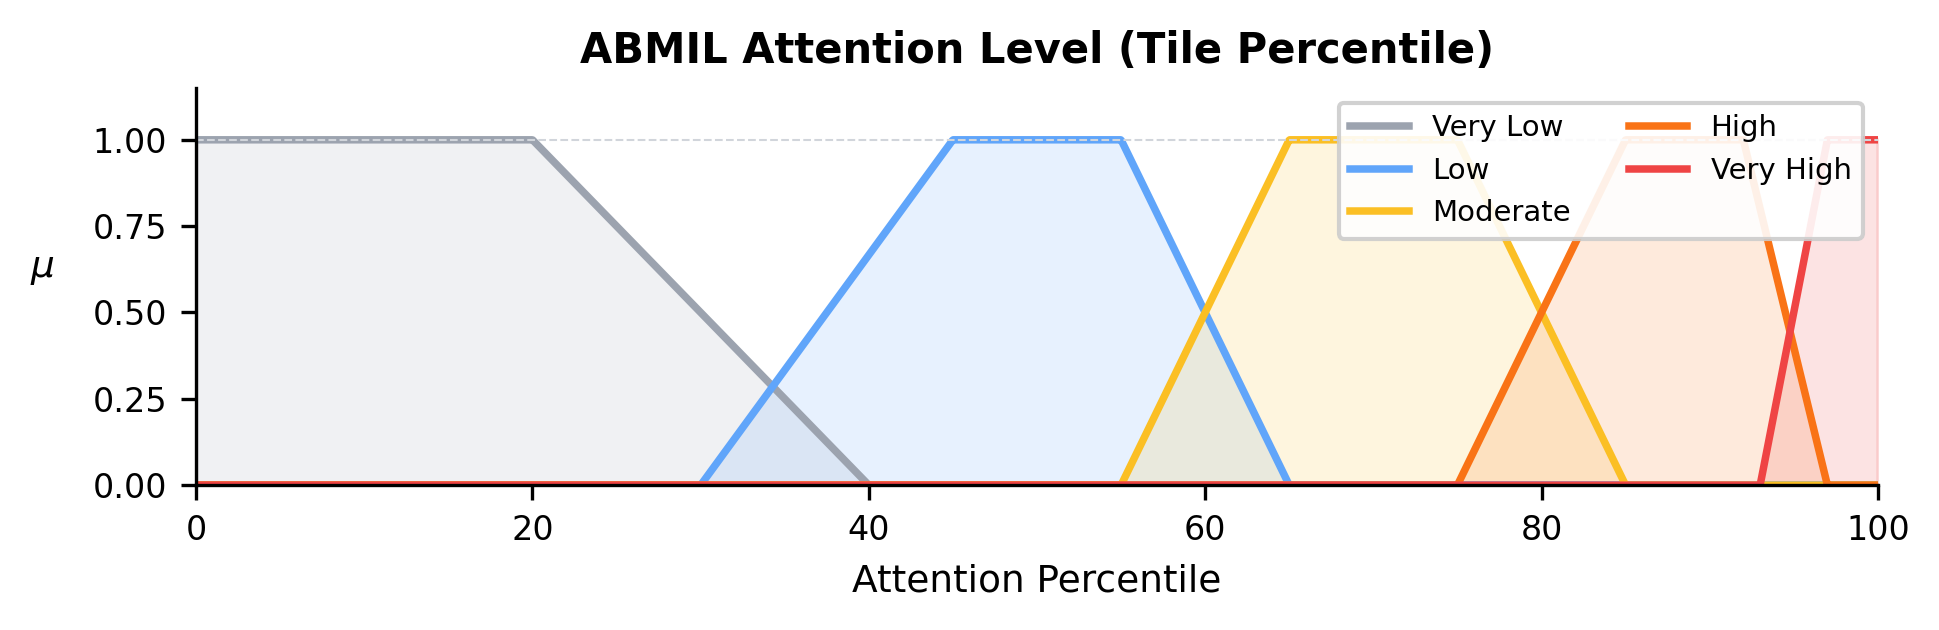
\includegraphics[width=\textwidth]{chapters/figures/fuzzy_mf_attention_level.png}
\end{minipage}
\caption[Trapezoidal membership functions for fuzzy linguistic XAI scales]{%
    Trapezoidal membership functions for the five fuzzy linguistic
    scales used to classify XAI outputs.
    Each scale maps a continuous input to overlapping fuzzy sets;
    the winning label (highest $\mu$) is displayed in the
    LCHAI~v2.0 interface and injected into LLM prompts.
    \textbf{Top left}: SHAP Balance (pattern contribution \%).
    \textbf{Top right}: Interaction Index ($|I_{jk}|$).
    \textbf{Middle left}: Shapley Profile (spread).
    \textbf{Middle right}: Shapley Individual ($|\delta_k|$).
    \textbf{Bottom}: ABMIL Attention Level (tile percentile).
    All thresholds are editable via the Admin panel
    (Section~\ref{sec:impl:lchai:fuzzy_labels}).}
\label{fig:fuzzy_mf_scales}
\end{figure}

The winning label (highest $\mu$) is injected verbatim into the LLM
prompt, creating a \textbf{dual anti-hallucination mechanism}: the KG
constrains \emph{what} the LLM says, and the fuzzy labels constrain
\emph{how} it says it.
All thresholds are configurable at runtime via the Admin panel.
This level extends fuzzy logic to a fourth pipeline layer:
(i)~training, (ii)~representation, (iii)~aggregation,
(iv)~interpretation.

\subsection{Human-in-the-Loop Pattern Correction (Active Learning)}
\label{sec:meth:active_learning}

The pattern classifier (Artefact~1) is trained on the Zenodo ANORAK
dataset, which may not fully represent the morphological diversity
encountered on clinical or TCGA slides.
LCHAI~v2.0 addresses this potential domain shift through a
\emph{human-in-the-loop} active learning mechanism that enables expert
pathologists to correct tile-level pattern classifications and trigger
incremental model refinement.

\textbf{Correction protocol (design).}
The expert pathologist annotates groups of misclassified tiles with
their correct pattern label.
At the methodological level the correction is a single object: a set
of tile indices and a target ANORAK class, persisted with provenance
metadata so that every corrected label is traceable to an expert and
a timestamp.
The concrete UI gesture (lasso, dropdown, ``Save \& Retrain'' button)
is reported in Section~\ref{sec:impl:lchai:ui:viewer}.

\textbf{Delta training formulation.}
Upon submission, the system performs \emph{head-only fine-tuning}:
the CTransPath backbone ($\sim$23M parameters) and the projection
head ($768 \to 512$) are frozen, and only the FuzzyArcLoss~V2 cosine
classification head ($\mathbf{W} \in \mathbb{R}^{6 \times 512}$,
$\sim$3{,}072 parameters) is updated.
The training data consists of the corrected tile embeddings
(expert-provided labels) augmented with a small buffer of original
tiles sampled from the same slide to prevent catastrophic forgetting.
The buffer ratio, the number of fine-tuning epochs, and the
fine-tuning learning rate are reported as implementation choices in
Section~\ref{sec:impl:lchai:ui:viewer}.

\textbf{Rationale for head-only fine-tuning.}
Fine-tuning the full backbone on a handful of corrected tiles
($\sim$50--500) would cause severe overfitting due to the
$23\text{M} \gg 500$ parameter-to-sample ratio.
By restricting updates to the 3{,}072-parameter classification head,
the effective model capacity is proportionate to the correction-set
size, and the pre-trained embedding space is preserved.
The same property makes delta training fast enough for interactive
clinical use without GPU access; the measured wall-clock time and
CPU-only execution mode are reported in
Section~\ref{sec:impl:lchai:ui:viewer}.

\textbf{Version management (design).}
Each delta-trained classifier is preserved as a new immutable version;
the original checkpoint is never overwritten, enabling rollback and
audit of all model versions.
After saving, the system automatically re-runs the inference pipeline
with the updated classifier, producing new pattern overlays and
mutation predictions.
The concrete object store (MinIO/S3) and the checkpoint-naming
convention are listed in Section~\ref{sec:impl:lchai:ui:viewer}.


\section{Multi-Ontology Knowledge Graph and Explanation Layer}
\label{sec:meth:ontology_method}
 
This section describes the methodology for the ontology-grounded
explanation layer of LCHAI~v2.0 (RQ6, RQ7).
The explanation layer does not participate in model training or mutation
prediction; it operates downstream as a semantic substrate that links
predicted mutation states to canonical biomedical knowledge.
 
\subsection{Ontology Integration}
\label{sec:meth:ontology:integration}
 
Two public biomedical ontologies provide the canonical entity
identifiers for the knowledge graph:
\begin{equation}
\label{eq:kg_union}
G = G_{\text{NCIt}} \cup G_{\text{MONDO}},
\end{equation}
where $G_{\text{NCIt}}$ is the NCI Thesaurus~\cite{sioutos2007ncit}
(providing IRIs for patterns, genes, diagnoses, and treatments) and
$G_{\text{MONDO}}$ is the Mondo Disease
Ontology~\cite{mondo_shefchek2020} (providing cross-disease linkage).
Rather than parsing the full OWL ontology files, the implementation
uses a \emph{curated edge store} in which each entity is identified
by its canonical IRI and each relationship edge carries a provenance
attribute citing its specific literature source
(Section~\ref{sec:impl:ontology:construction}).
 
The unified graph encodes the relation chain:
\begin{equation}
\label{eq:kg_chain}
\text{pattern} \xrightarrow{\texttt{assocWithMutation}}
\text{gene} \xrightarrow{\texttt{treatedWith}}
\text{therapy},
\end{equation}
grounded in canonical IRIs (Table~\ref{tab:iri_mapping}).
 
\begin{table}[ht!]
\centering
\small
\caption{Canonical IRI assignments for LUAD knowledge graph entities.}
\label{tab:iri_mapping}
\begin{tabular}{l l l l}
\hline
\textbf{Entity} & \textbf{Type} & \textbf{Ontology} & \textbf{Code} \\
\hline
Lepidic pattern       & Pattern   & NCIt  & C55821  \\
Acinar pattern        & Pattern   & NCIt  & C35922  \\
Papillary pattern     & Pattern   & NCIt  & C35911  \\
Micropapillary pattern & Pattern  & NCIt  & C36181  \\
Solid pattern         & Pattern   & NCIt  & C36182  \\
Cribriform pattern    & Pattern   & NCIt  & C35920  \\
\hline
EGFR  & Gene & NCIt & C17757  \\
KRAS  & Gene & NCIt & C25785  \\
TP53  & Gene & NCIt & C17359  \\
STK11 & Gene & NCIt & C18253  \\
KEAP1 & Gene & NCIt & C112105 \\
RBM10 & Gene & NCIt & C115382 \\
\hline
Adenocarcinoma & Diagnosis & NCIt  & C2852    \\
NSCLC          & Diagnosis & MONDO & 0005233  \\
\hline
Osimertinib  & Treatment & NCIt & C116377 \\
Sotorasib    & Treatment & NCIt & C154287 \\
Alectinib    & Treatment & NCIt & C101790 \\
\hline
\end{tabular}
\end{table}
 
\subsection{Three-Layer Architecture and Query Flow}
\label{sec:meth:ontology:layers}
\label{sec:meth:ontology:sparql}

At inference time, the knowledge graph is queried as a three-layer
stack and the resulting case-specific subgraph is then injected as
context into every downstream LLM call
(Figure~\ref{fig:edge_store_query_flow}).
The three layers play complementary epistemic roles:

\textbf{Vocabulary scope.}
The \emph{static} curated layer (Layer~1) uses five relation types
(\texttt{subtypeOf}, \texttt{associatedWithMutation},
\texttt{treatedWith}, \texttt{mutatedIn}, \texttt{equivalentClass};
see Section~\ref{sec:impl:ontology:construction}).
The \emph{open} DeepSearch vocabulary (Layer~3) additionally admits
\texttt{resistantTo} and \texttt{biomarkerFor}, which encode
\emph{negative} therapeutic and \emph{predictive} biomarker relations
that only become meaningful as new literature accrues, and therefore
consists of six predicates.
The expansion is intentional: Layer~1 captures only relations with
sufficient curated evidence at thesis-publication time; Layer~3 must
ingest a broader vocabulary so the KG can grow.

\textbf{Layer~1 --- Curated assertions.}
A small, version-controlled set of edges encodes established clinical
evidence. Each entity is identified by its canonical NCIt or MONDO
IRI (Table~\ref{tab:iri_mapping}); each edge carries a
\texttt{provenance} attribute pointing to a PMID (for pattern--gene
correlations) or an authoritative source such as OncoKB/FDA (for
gene--therapy edges).
The exact edge inventory, the literature provenance per edge, and the
fact that two patterns (acinar, cribriform) carry \emph{no}
\texttt{associatedWithMutation} edges by deliberate omission are
catalogued in Section~\ref{sec:impl:ontology:construction}.

\textbf{Layer~2 --- Dynamic case filter.}
At query time the traversal of Layer~1 is filtered against the
current case so that only patterns with non-trivial composition,
genes reachable from those patterns or predicted
positive/inconclusive, and their associated therapies survive.
The substantive design property is that the merged subgraph reflects
the morphology actually observed on the slide rather than the
universe of all possible LUAD relations---for example, a case
dominated by solid and micropapillary morphology produces a subgraph
centred on TP53 and KRAS, not on EGFR inhibitors.

\textbf{Layer~3 --- Literature-discovered relations.}
Relations produced by the DeepSearch batch pipeline
(Section~\ref{sec:meth:deepsearch}) are merged into the case subgraph
as \emph{inferred} edges, distinguished from Layer~1's \emph{asserted}
edges so that downstream consumers (the LLM, the Graph-tab UI, the
audit log) can treat the two epistemic statuses differently.
The persistence backend (a relational table with an active/inactive
flag) and the administrator-facing deactivation workflow are reported
in Section~\ref{sec:impl:ontology:runtime}.

\textbf{Graph assembly and LLM grounding.}
The Layer~1+2 subgraph and the active Layer~3 relations are merged
into a single case-specific JSON graph that is injected into every
LLM prompt with the instruction to use \emph{only} these edges for
clinical associations.
This design enforces three properties:
(a)~explanations evolve automatically as DeepSearch discovers new
relations,
(b)~the LLM cannot fabricate clinical associations absent from the
verified KG, and
(c)~all intensity terms are pre-computed by the fuzzy linguistic
label system
(Level~6, Section~\ref{sec:meth:interp:fuzzy_labels}) and injected
verbatim, so the LLM never invents qualitative wording either.
Clinical guardrails (e.g.~prohibition of phrases such as
``confirmed diagnosis'') keep outputs within the system's intended
role as a research/decision-support tool.
Migration to a formal triplestore with SPARQL endpoints is
identified as medium-term future work
(Section~\ref{sec:disc:future:medium}).

\begin{figure}[!htbp]
\centering
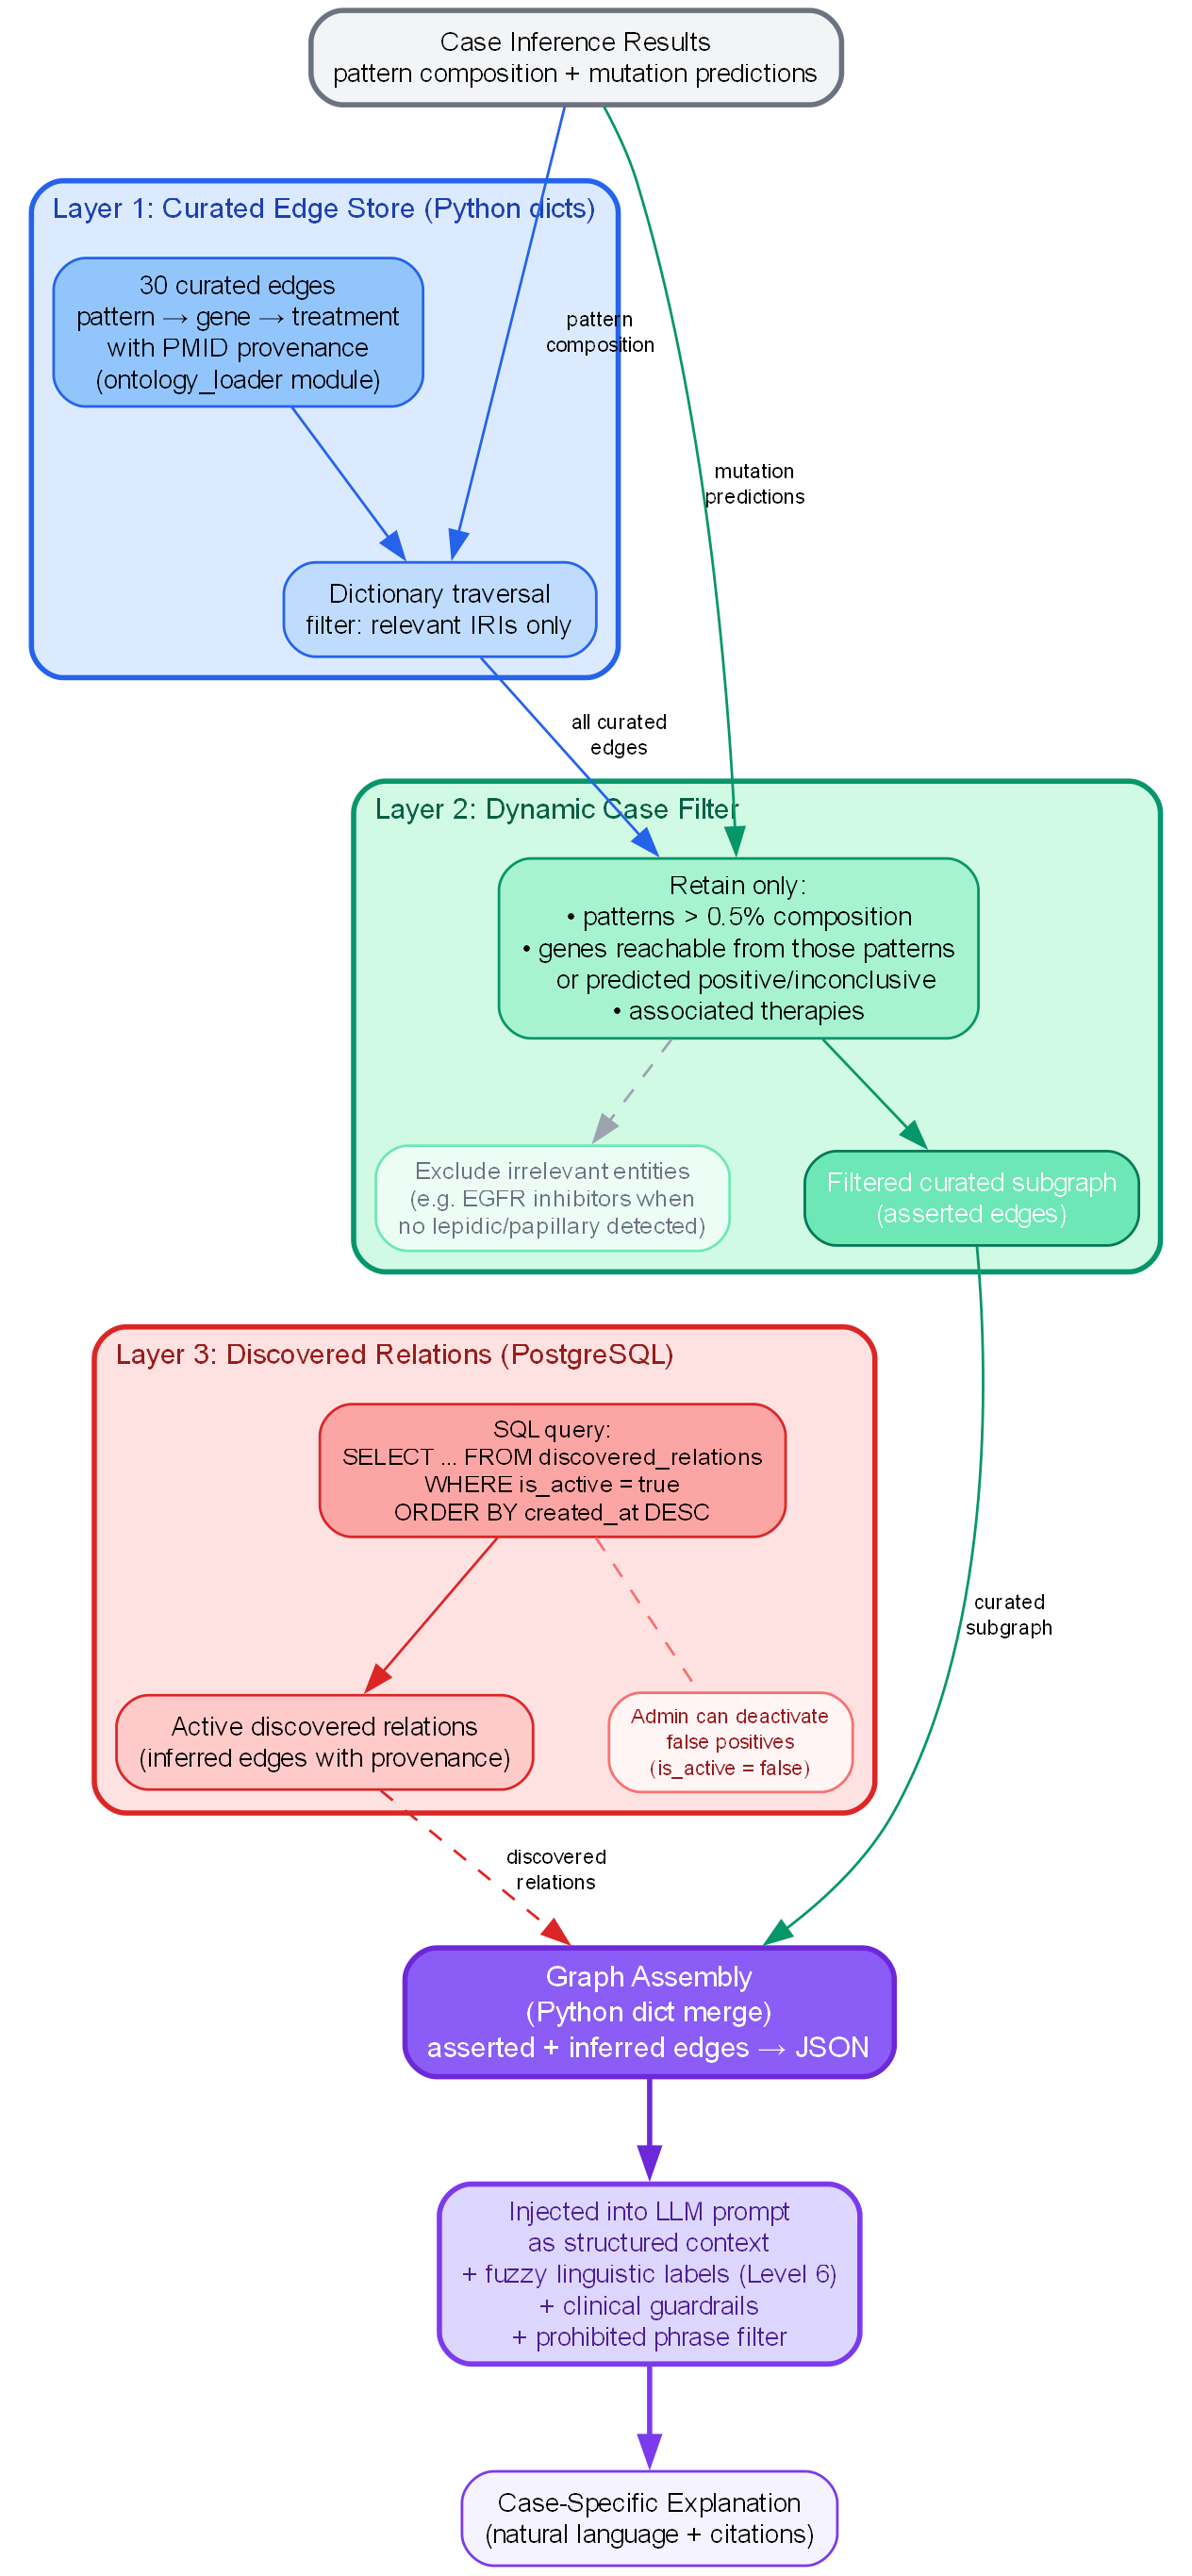
\includegraphics[width=0.62\textwidth]{chapters/figures/edge_store_query_flow.png}
\caption[Three-layer KG architecture and query flow]{%
    Three-layer knowledge graph architecture and query flow.
    \textbf{Layer~1} (blue): 30 curated edges with PMID provenance.
    \textbf{Layer~2} (green): dynamic case filtering retains only
    patterns, genes and therapies relevant to the case.
    \textbf{Layer~3} (red): DeepSearch-discovered relations retrieved
    from PostgreSQL (\texttt{is\_active = true}).
    \textbf{Graph assembly} (purple): asserted and inferred edges are
    merged into a JSON graph, injected into the LLM prompt with fuzzy
    linguistic labels (Level~6) and clinical guardrails.}
\label{fig:edge_store_query_flow}
\end{figure}

\subsection{DeepSearch: Continuous Knowledge Enrichment}
\label{sec:meth:deepsearch}

The DeepSearch pipeline addresses a methodological gap left open by
Layer~1: a curated edge store frozen at thesis-publication time would
quickly become stale relative to the LUAD literature.
The methodological design is a six-stage batch pipeline that
(i)~queries the literature, (ii)~extracts candidate relations via an
LLM under a constrained predicate vocabulary, (iii)~links extracted
entities to canonical IRIs, (iv)~deduplicates triples,
(v)~enforces type-constraint validity, and (vi)~persists the survivors
under version control.
The substantive design properties at this layer are
\emph{constrained generation} (the LLM is restricted to a fixed
predicate vocabulary so it cannot invent new edge types),
\emph{symbolic verification} (every triple must pass type-constraint
validation before persistence), and \emph{reversible curation}
(administrators can deactivate false-positive triples without
destroying the audit record).
The concrete query bank, LLM backend, type rules and storage
backend---together with the run-time success criterion for RQ7---are
reported in Section~\ref{sec:impl:ontology:deepsearch} and
Section~\ref{sec:eval:lchai}.

A representative failure mode that motivates the
deactivation-without-deletion design is the
acinar/KRAS co-occurrence: a paper mentioning ``acinar'' and ``KRAS''
in the same abstract does not imply a positive association---pooled
evidence shows an inverse relationship,
OR~$= 0.65$, $p < 0.01$~\cite{ejso2019pooled}.
Without an explicit administrator override, even a type-correct triple
of this form would otherwise propagate into the LLM prompt.

% ============================================================================
\section{Evaluation Protocol}
\label{sec:meth:evaluation_protocol}
% ============================================================================

\subsection{Cross-Validation Strategy}
\label{sec:meth:eval:cv}

\subsubsection{Pattern Classification (Artefact 1)}

The pattern classifier is evaluated using 5-fold stratified cross-validation
repeated with 3 random seeds, yielding 15 runs per method.
Stratification ensures that the class distribution (including the minority
cribriform and micropapillary classes with $\sim$69 tiles each;
Table~\ref{tab:dataset_config_anorak}) is preserved in each fold.
Results are reported as mean $\pm$ standard deviation of macro-F1 across the
15 runs.

\subsubsection{Mutation Prediction (Artefacts 2 and 3)}

The mutation prediction benchmark uses 5-fold \emph{patient}-stratified
cross-validation on the 687 LUAD slides (668 unique patients).
Because 19 patients contribute more than one slide, stratification is applied
at the patient level to prevent data leakage between training and test folds.
Concretely, all slides from a given patient are assigned to the same fold.
The binary mutation label is used to preserve the per-gene mutation prevalence
across folds.

For genes with low prevalence, the expected number of positive cases per fold
is as follows:
\begin{itemize}
    \item \textit{RBM10} (5.4\%, 37 mutated): $\approx$7 positive cases per fold.
    \item \textit{STK11} (9.9\%, 68 mutated): $\approx$14 positive cases per fold.
    \item \textit{EGFR} (11.4\%, 78 mutated): $\approx$16 positive cases per fold.
\end{itemize}

These counts are sufficient for AUROC estimation but contribute to the
high fold-to-fold variance (std 0.05--0.10) observed in the results.

$K = 5$ was chosen over $K = 10$ because the latter would produce folds
with only $\sim$3--4 positive cases for RBM10---below the minimum for
reliable AUROC estimation---and $\sim$7 for STK11, which is marginal.

All six experimental conditions (B1: XGBoost floor baseline;
B2: ABMIL ceiling baseline on embeddings; B3: ABMIL on patterns;
PI-ABMIL, ours; A: crisp ablation; FC-MIL, ours) share the same
fold splits.
Conditions B2, B3, PI-ABMIL and A evaluate Artefact~2 under different
input representations, while condition FC-MIL evaluates Artefact~3.

\subsection{Metrics}
\label{sec:meth:eval:metrics}

\textbf{Primary metric:} AUROC (Area Under the Receiver Operating
Characteristic Curve), the standard metric in the mutation prediction
literature~\cite{coudray2018classification,kather2020pancancer}, reported as mean $\pm$ standard deviation across folds.

\textbf{Secondary metrics:} AUPRC~\cite{davis2006auprc} (Area Under the Precision-Recall
Curve), particularly informative for imbalanced genes (RBM10 at 5.4\%,
STK11 at 9.9\%);
and F1 score at the 0.5 probability threshold, with the caveat that
threshold optimisation (e.g., Youden's $J$~\cite{youden1950index}) would be needed for
clinical deployment.
AUPRC is computed for all six experimental conditions to expose
the gap between ranking ability and precision-recall performance,
especially for low-prevalence genes (see Figure~\ref{fig:auprc_by_gene}).
The primary comparison across all six conditions relies on AUROC,
as the models are not calibrated and F1 at a fixed threshold of 0.5
does not reflect their true discriminative ability
(see Section~\ref{sec:disc:lim:method}).

\textbf{Pattern classification metric:} Macro-F1, which weights all six
classes equally regardless of prevalence, penalising models that sacrifice
minority classes (especially cribriform) for overall accuracy.

\paragraph{Conclusive vs Inconclusive verdict.}
Independently of the per-fold metrics above, a binary
deployment-readiness label is assigned \emph{per gene at the cohort
level} (a population-level reliability flag, not a per-slide
attribute): a gene is declared \emph{Conclusive} if and only if its
held-out 5-fold cross-validated mean AUROC clears a fixed
discrimination floor, and \emph{Inconclusive} otherwise.
The verdict is derived \emph{from AUROC alone} (a prevalence-aware
extension that also incorporates AUPRC is identified as future work
in Chapter~\ref{ch:discussion}); AUPRC is reported in parallel as a
secondary metric for interpretation, not as part of the gating
criterion.
This per-gene flag propagates into the LCHAI~v2.0 user interface,
gating which genes surface a probability number versus which surface
only a calibration warning---it is therefore a property of a gene's
signal under the proposed architecture, orthogonal to any per-slide
prediction.
The concrete threshold value, the calibration test
(Hosmer--Lemeshow) and the per-gene assignment under the present
benchmark are reported in
Section~\ref{sec:impl:lchai:confidence} and corroborated by the
empirical numbers in Chapter~\ref{ch:evaluation}.

\subsection{Statistical Testing}
\label{sec:meth:eval:testing}

\subsubsection{Paired $t$-Test}

For comparing two conditions on the same folds, a paired two-tailed $t$-test is applied to the fold-level AUROC values.
With $K = 5$ folds, the test has limited statistical power; significance at $p < 0.05$ therefore represents a strong result.

\subsubsection{Cohen's $d$ Effect Size}

To complement $p$-values, Cohen's $d$ quantifies the standardised difference between two conditions:
\begin{equation}
\label{eq:cohens_d}
d = \frac{\bar{x}_1 - \bar{x}_2}{s_{\text{pooled}}},
\end{equation}
where $s_{\text{pooled}}$ is the pooled standard deviation.
Following standard conventions~\cite{cohen1988statistical}: $|d| < 0.2$ = negligible, $0.2 \leq |d| < 0.5$ = small, $0.5 \leq |d| < 0.8$ = medium, $|d| \geq 0.8$ = large.

\subsubsection{Win Rate}

For the pattern classifier (15 runs), the win rate reports the fraction of runs in which condition A outperforms condition B.
A win rate of $\geq 13/15$ (86.7\%) provides strong evidence of consistent superiority beyond random variation.

\subsection{Ablation Design}
\label{sec:meth:eval:ablation}

The experimental conditions form a structured ablation in which each
question changes a \emph{single} design variable (or, for
question~4, a controlled pair of jointly varying variables on a
fixed information source) while holding all other components
constant:
\begin{enumerate}
    \item \textbf{Does pattern information help at all?}
    The hypothesis $\text{PI-ABMIL} > B2$ would indicate that patterns
    add discriminative value on top of embeddings, and $B3 >
    \text{chance}$ (AUROC $> 0.5$) that patterns alone carry
    signal.
    The empirical answer is reported in
    Sections~\ref{sec:eval:mutation:finding1}
    and~\ref{sec:eval:mutation:finding5}: $B3 > \text{chance}$ holds
    universally, but $\text{PI-ABMIL} > B2$ holds only for a
    structural subset of genes (cohort-level tie, gene-dependent).

    \item \textbf{Are embeddings necessary alongside patterns?}
    The companion hypotheses are $\text{PI-ABMIL} > B3$
    (embeddings add value on top of patterns) and $B2 > B3$
    (embeddings alone outperform patterns alone).
    Together with question~1, this pair tests whether the two
    information sources are complementary rather than redundant; the
    empirical outcome is reported in
    Section~\ref{sec:eval:mutation:finding1} (both inequalities hold
    at the cohort level, with RBM10 as the only per-gene reversal).

    \item \textbf{Are soft (fuzzy) probabilities better than hard
    (crisp) labels?}
    Test $\text{PI-ABMIL} > A$.
    Both conditions share the same 518-d input dimension and the same
    ABMIL architecture; the only variable that changes is whether the
    pattern channel carries the full softmax distribution
    $\mathbf{p}_i \in \Delta^5$ or its $\arg\max$ one-hot encoding
    $\mathbf{o}_i \in \{0,1\}^6$.
    The empirical answer is reported in
    Section~\ref{sec:eval:mutation:finding3}.

    \item \textbf{Does tile-level MIL add value over slide-level
    aggregation?}
    Test $B3 > B1$.
    Both conditions consume only pattern information, so the
    representation source is held fixed; the \emph{two} variables
    that change jointly are (i) the aggregator (gated-attention MIL
    vs gradient-boosted XGBoost) and (ii) the input granularity
    (tile-level fuzzy memberships vs slide-level pattern fractions).
    The pair is therefore a joint test of MIL aggregation
    \emph{plus} fine-grained tile-level evidence over a single
    coarse slide-level summary.
    The contrast $B2 > B1$ is intentionally \emph{not} used as the
    MIL test because it confounds an additional third variable
    (representation: embeddings vs patterns) and therefore cannot
    attribute any observed gain to MIL alone.
    The empirical answer is reported in
    Section~\ref{sec:eval:mutation:finding5}.

    \item \textbf{Does the Choquet branch add value over
    concatenation?}
    Test FC-MIL vs PI-ABMIL per gene.
    Because FC-MIL shares the embedding pathway with ABMIL, this
    comparison isolates the contribution of the Choquet aggregation
    over standard attention pooling.
    FC-MIL additionally provides intrinsic interpretability (Shapley
    values and interaction indices) absent from PI-ABMIL; Shapley
    interaction analysis provides a qualitative plausibility check
    against known biology.
    The empirical answer is reported in
    Section~\ref{sec:eval:mutation:finding6}.
\end{enumerate}

By construction, each comparison changes a single design variable
(or, for question~4, a controlled pair of jointly varying variables
on a fixed information source) while keeping the remaining components
fixed, enabling attribution of performance gains (or losses) to
individual design decisions rather than to confounded combinations
of them.


% ============================================================================
\section{Chapter Summary}
\label{sec:meth:summary}
% ============================================================================

This chapter has presented the complete methodology for the three
computational artefacts, the interpretability framework, and the
ontology explanation layer:

\textbf{Artefact~1 (FuzzyArcLoss~V2)} introduces a per-sample fuzzy
membership coefficient $\mu_i$ that interpolates between the ArcFace
target logit and the margin-free cosine, derived from a piecewise
linear function of classification confidence.
The four membership coefficients ($a_H = 0.8$, $b_H = 0.2$,
$a_L = 0.3$, $b_L = 0.4$) are determined by three design
principles---high-confidence floor, positive global floor, and
doubled gradient sensitivity for ambiguous samples
(Table~\ref{tab:coeff_derivation})---and the gradient analysis
confirms that V2 produces a smoother optimisation landscape at
morphological boundaries than standard ArcFace.
A combined loss (label-smoothing CE $+$ focal loss) complements the
margin modulation to handle class imbalance.
Optuna hyperparameter optimisation identified an aggressive scale
($s = 46.1$) compensated by the fuzzy safety valve.
Two ablation variants were specified: V3 (sub-centre extension,
which underperforms V2 due to overfitting on 55--145 tiles/class) and
V2~ClassParams (per-class margin geometry, excluded from K-fold due
to search space cost).

\textbf{Artefact~2 (Pattern-Informed ABMIL)} concatenates CTransPath
512-d embeddings with 6-d fuzzy pattern probability vectors to create
enriched 518-d tile representations.
The gated attention MIL mechanism learns which tiles are most
informative for mutation prediction, while the pattern channel provides
an explicit biological prior.

\textbf{Artefact~3 (Fuzzy Choquet MIL)} augments the shared ABMIL
embedding pathway with a parallel Choquet integral branch operating on
fuzzy pattern memberships under a learned 2-additive fuzzy measure.
The 21-parameter fuzzy measure provides built-in interpretability
through Shapley values and interaction indices
(Figure~\ref{fig:choquet_interpretability}), while the shared encoder
ensures that capacity differences do not confound the comparison.

\textbf{Six-level interpretability framework.}
Spatial attention maps (Level~1), pattern overlays (Level~2), SHAP
decomposition (Level~3), Choquet Shapley values (Level~4), per-slide
feature channel ablation (Level~5), and fuzzy linguistic labels
(Level~6) provide complementary \emph{interpretability outputs} for
every prediction---structural inspection of the model itself, in
the sense of Section~\ref{sec:bg:xai:definitions}.
The fuzzy labels, computed by trapezoidal membership functions and
injected verbatim into LLM prompts, form a dual anti-hallucination
mechanism alongside the knowledge graph.

\textbf{Ontology-grounded explainability layer.}
Separate from the interpretability framework, a three-layer
knowledge graph (curated edge store, dynamic case filter,
DeepSearch-discovered relations) supplies the
\emph{explainability} component of LCHAI~v2.0 (RQ6, RQ7): it
links predictions to canonical biomedical knowledge with PMID
provenance and grounds the LLM-generated natural-language
rationales presented to the end user.
Its formal evaluation against expert
preferences is identified as future work
(Section~\ref{sec:bg:xai:definitions}).

\textbf{Evaluation protocol.}
Five-fold patient-stratified cross-validation with AUROC as the
primary metric, paired $t$-tests and Cohen's $d$ for statistical
comparison, and a structured five-comparison ablation design using
floor (B1) and ceiling (B2) baselines.

Chapter~\ref{ch:implementation} describes the software implementation
of these artefacts, and Chapter~\ref{ch:evaluation} presents the
evaluation results.
